\documentclass[]{book}

\title{\textbf{Quantum Computation and Quantum Information}}
\author{Hsi-Sheng Goan}
\date{}

\usepackage{verbatim}
\usepackage{multirow}
\usepackage{multicol}
\usepackage{amsmath,amsfonts,amssymb,amsthm}
\usepackage{braket}
\usepackage[margin=1.0in]{geometry}
\usepackage{bbold}
\usepackage{enumitem}
\usepackage{mdframed}
\usepackage{ntheorem}
\usepackage{commath,mathtools}
\usepackage{dsfont}
\usepackage{qcircuit}

\newtheorem*{remark}{Remark}
\newtheorem*{propos}{Proposition}
\newtheorem*{example}{Example}
\theoremstyle{nonumberplain}
\newmdtheoremenv{definition}{Definition}
\newmdtheoremenv{theorem}{Theorem}
\newmdtheoremenv{postu}{Postulate}

\begin{document}
\maketitle
\tableofcontents

\begin{comment}
\section{Overview}
\label{sec:overview}
	53 quantum bits (Quantum supremency)\\
	Task that super computer takes 100000 years (IBM days) only takes 200 sec on Quantum Computer\\
	IBM 53 qubits have not been optimized\\
	$2^{100}$ state seems powerful \\
\section{Speech}
RSA cryptography: Factor two prime number
Factor 309-digit number: Classical THz computer take 150000 years, and quantum computer take $<$ 1s
\subsection{Quantum bit}
Classical bit: 0 or 1\\
Quantum bit: QM two-state system $\ket{\psi}=\alpha\ket{0}+\beta\ket{1}$\\
Two qubit: We can have four state simultaneously $\ket{\psi}=\alpha\ket{00}+\beta\ket{01}+\gamma\ket{10}+\tau\ket{11}$\\
So in quantum register, for 3 bit, we can have 8 states simultaneously,unlike classical register only 1 state
\subsection{Development}
2016 IBM 5-qubit online\\
2017 IBM 16-qubit online (but 1 or 2 malfunction)\\ 
50 qubits need to pay
The temperature for Quantum computer is nearly 20mK to superconduct\\
Noisy Intermediate Scale Quantum $(NISQ)$\\
In classical computer, we can prevent noise just put on threshold, but quantum error is hard to correct. We may add another error to that\\
Google v.s. IBM: 53 qubits 200s and 72 petabyte momory few days
\subsection{implementation}
\begin{itemize}
\item 1998 proposol: Sillicon-based electron-immediated nuclear spin (2012 implement)
\item  Electron spins in quantum dots
\item	2015 two-quibt logic gate in silicon (Using semiconductor 15nm!!)
\end{itemize}
\subsection{Challenge}
\begin{itemize}
	\item Much larger numbers of qubits e.g. shor's need thousand qubits
	\item	Much greater connectivity with fewer restriction
	\item Much lower error rate
	\item True fault tolerance-error correction
	\item Higher operating temperture
\end{itemize}
\subsection{HQC}
Hybrid Quantum-Classical (HQC) Algorithm\\
Variational quantum circuit algorithm\\
Data encoding scheme\\
Vairational Quantum Eigensolver (VQE)
\subsection{Application}
\begin{itemize}
	\item Artificial intelligence
	\item Medicine and Materials (Molecule simulation)
	\item Supply chain
	\item Cloud Security
\end{itemize}

\end{comment}

\chapter{Quantum Computation \& Quantum Information (QC\&QI)}%
\label{sec:quantum_computation_quantum_information}
It is the study of information processing and computing tasks that can be accomplished using QM system.
\begin{remark}
IBM using classical approach to simulate 32 qubits QM system. 
\end{remark}
\begin{remark}
Quantum system is rare in our daily life. It seems the nature is against it.
\end{remark}
\begin{flushleft}
Explore and exploit Quantum effect, based on the principle of QM to compute and process information in ways that are \textbf{faster} or \textbf{more efficient} than or \textbf{even impossible} on conventional computers or information processing devices.
\end{flushleft}
\begin{example}
\ \\
Shor's Quantum factoring algorithms (1994)\\
Grover's Quantum search algorithms (1996)\\
Quantum simulation (exponential enhancement in memory size) Feynamn 1982\\
Quantum Teleportation (1993) Bennett et al.\\
Quantum superdense coding (1992)Bemett and Wiesner \\
Quantum Cryptography (Quantum Key Distribution) (1984) Bennett and Brassard
\end{example}
\begin{remark}
\textbf{Only} Quantum machine can simulate quantum system. Because quantum system grows too fast.
\end{remark}
\begin{remark}
Quantum Teleportation: Transfer quantum state from one place to another place \\
Quantum superdense coding: Use a few qubit to transfer more bit information
\end{remark}
\begin{remark}
Shor's: Prime factorization, exponential speed up\\
Grover's: Unsorted data, quadratic speed up\\ 
\end{remark}
\begin{center}
What is the killer application ?
\end{center}
\chapter{Quantum Information Sciences (QIS)}%
\label{sec:quantum_information_sciences}
To catch all aspectes of QC \& QI
\section*{Fundamental Questions of IS}
\begin{enumerate}
	\item \label{IS:first} Given a physical resoures - energy, time, space, bit, gates
	\item \label{IS:second} Given an information processing task - data compression, information transmission, computing task, factoring
	\item \label{IS:third} Given a criterion for success
\end{enumerate}
We ask the question: How much of \ref{IS:first} do I need to achieve \ref{IS:second} while satisfying \ref{IS:third} ?
\\
\\
Pursuing this question in the quantum case has led to and presumably will continue to lead to interesting new information processing capability.
\section*{Knowing The Rules of QM $\neq$ Understanding the QM}
\paragraph{What high-level principles are implied by QM?}
\textit{To discuss these high-level principles, we may need to know the basic rules of QM first.}\\
QM has a fearsome popular image because the mathematics required to apply QM to problems like determining the energy spectra of molecules and calculating scattering cross-section is difficult or intimidating.\\
\\
By contrast, the mathematics used in application to QIS is "relatively painless". Do not need to read the tranditional QM textbooks. Here, I mean the mathematics required to understand those algorithms protocols. However, the math for physical implementation and consideration of real world, noise and decoherence may be a little bit involved.\\

\paragraph{What is Quantum Mechanics?}
    \textit{Is it a complete physical theory of the world in its own right? No!! misconception!!} \\
	It is a mathematical and conceptual  framework for the development of physical theory.
\paragraph{QM consists of a set of mathematical postulates:}
\label{par:qm_consists_of_a_set_of_mathematical_postulates_}
\begin{center}
Surprisingly, 4 simple postulates which lay the ground rules for our description of the world.\\
\end{center}
Most physicists believe that theory of everything will be a QM theory:
\begin{enumerate}
	\item Attempts to describe gravitation in the framework of QM has so far not yet been successful.
	\item Conceptual issue, so called "measurement problem" remains to be clarified.
\end{enumerate}
\section{The Structure of QM for QIS}
\label{sec:the_structure_of_qm_for_qis}
\begin{equation*}
\begin{cases}
	\textit{linear algebra: Matrix, finite-dimension}\\
	\textit{Dirac notation:} \ket{\psi}, \bra{\psi}=\ket{\psi}^{\dagger}, \langle A \rangle = \braket{\psi|A|\psi}\\
	\textit{4 postulates of QM}
\end{cases}
\end{equation*}
\begin{enumerate}
	\item How to describe Quantum state of a closed system? \\
		State space (Hilbert space), state vector
	\item How to describe Quantum dynamics (time evolution)? \\
		Unitary evolution
	\item How to describe measurements of a Quantum system? \\
		Projective measurement $\rightarrow$ POVM measurement, Generalized Quantum measurement
	\item How to describe Quantum of a composite system? \\
		tensor product
\end{enumerate}
\section{The Postulates of Quantum Mechanics}
\subsection{State Space}
\begin{postu}[1]
	Associated to any isolated physical system is a complex vector space with inner product (that is Hilbert space) known as the state space of the system. The system is completely described by its state vector which is a unit vector in the system's state space.
\end{postu}
\begin{remark}
QM does not tell us, for a given physical system, what the state space of that system is, nor does it tell us the state vector of the system is.
\end{remark}
\begin{remark}
	Finding that out for a specific system is a difficult problem for which physicists have developed many beautiful rules (e.g. QED)
\end{remark}
\begin{example} 
	\textbf{Quantum bit (qubit) (Two level (orthonormal basis states) system)}\\
"bit" is the fundamental element for information processing concept of classical Computation and Information. It can exist in two distinct states represented by 0 and 1.\\
It is over $\mathbb{C}^{2}$ and quantum state is just a unit vector in that space.
\[
\ket{\psi}=\alpha\ket{0}+\beta\ket{1}
\] 
\[
\ket{\psi} = \alpha\ket{0}+\beta\ket{1} = 
\begin{pmatrix}
\alpha \\
\beta
\end{pmatrix}_{in\  \ket{0}, \ket{1}\ basis}
= \alpha
\begin{pmatrix}
1\\
0
\end{pmatrix}
+ \beta
\begin{pmatrix}
0\\
1
\end{pmatrix}
\] 
\[
	\braket{\psi|\psi} = 
\begin{pmatrix}
	\alpha^{*} & \beta^{*}
\end{pmatrix}
\begin{pmatrix}
	\alpha\\ \beta
\end{pmatrix}
= \abs{\alpha}^{2}+\abs{\beta}^{2}=1
\] 
\end{example}
\subsection{Evolution}
\begin{postu}[2]
The evolution of a closed Quantum system is described by a unitary transformation
\[
	\ket{\psi(t_{2})}=U(t_{1},t_{2})\ket{\psi(t_{1})}
\]
\end{postu}
\begin{remark}
    Unitary map is the only linear map that preserves normalization. 
    \[
     \text{Unitary: } U^{\dagger}U = I_{N\times N}
    \]
    \[
     \bra{\psi(t_{2})} = \bra{\psi(t_{1})}U^{\dagger}(t_{1},t_{2})
    \]
    \[
    \braket{\psi^{\prime}|\psi^{\prime}}=\braket{\psi^{\prime}|U^{\dagger}U|\psi^{\prime}}
    =\braket{\psi|\psi}
    \]
\end{remark}
\begin{remark}
	QM does not prescribe this unitary evolution for particular system. Physicists figure it out by a complex interplay between theory and experiment
\end{remark}
\begin{remark}
matrix = transformation = linear operator = map = Quantum gate
\end{remark}
\begin{example}
	Pauli gate (Pauli sigma matrices) \\
\[
\sigma_{x}=
\begin{pmatrix}
	0 & 1\\
	1 & 0
\end{pmatrix}
\ \sigma_{y}=
\begin{pmatrix}
	0 & -i\\
	i & 0
\end{pmatrix}
\ \sigma_{z}=
\begin{pmatrix}
	1 & 0\\
	0 & -1 
\end{pmatrix}
\ \mathds{1}=
\begin{pmatrix}
	1 & 0\\
	0 & 1 
\end{pmatrix}
\] 
\begin{figure}[!hbt]
	\centering
	\includegraphics[scale=0.5]{graph/1.png}
\end{figure}
\\
Quantum wire: The qubit is carried along by this Quantum wire until it reaches the X gate, not necessarily means that it carries qubit through space, may represent a stationary qubit which is simply sitting there, passing through time until the X gate is applied.
\begin{equation*}
\begin{aligned}
	X\ket{0} &= 
\begin{pmatrix}
	0 & 1 \\
	1 & 0 
\end{pmatrix}
\begin{pmatrix}
1 \\
0
\end{pmatrix}
=
\begin{pmatrix}
0 \\
1
\end{pmatrix}
=\ket{1} 
\\
X\ket{1} &= 
\begin{pmatrix}
	0 & 1 \\
	1 & 0 
\end{pmatrix}
\begin{pmatrix}
0 \\
1
\end{pmatrix}
=
\begin{pmatrix}
1 \\
0
\end{pmatrix}
= \ket{0}
\end{aligned}
\end{equation*}
\begin{center}
Quantum NOT gate
\end{center}
\end{example}
\begin{postu}[2']
	The time evolution of the state of a closed (non-relativistic) quantum system is described by Schr$\ddot{o}$dinger equation:
\[
i\hbar\frac{\partial \ket{\psi}}{\partial t} = \mathcal{H}\ket{\psi}
\] 
if $\mathcal{H}$ is independent of time
\[
	U(t_{1},t_{2}) = e^{-i\mathcal{H}(t_{2}-t_{1})/\hbar}
\] 
if $\mathcal{H}$ depends on time, we have to do the integration on Hamiltonian
\end{postu}
\subsection{Quantum Measurement}
\begin{postu}[3. General Measurement]
	Quantum measurements are described by a collection $\{M_{m}\}$ of measurement operators. There are operators acting on the state space of the system being measured. The index m refers to the measurement outcomes that may occur in the experiment. If the state of the quantum system is $\ket{\psi}$ immediately before the measurement then:
\begin{enumerate}
	\item The probability that result m occurs is given by 
		\[
			p(m) = \braket{\psi|M_{m}^{\dagger}M_{m}|\psi}
		\] 
	\item And the state of the system after the measurement is 
		\[
			\frac{M_{m}\ket{\psi}}{\sqrt{\braket{\psi|M_{m}^{\dagger}M_{m}|\psi}}}
		\] 
\end{enumerate}
The measurement operators satisfy the completeness equation $\sum^{}_{m} M^{\dagger}_{m}M_{m}=\mathds{1}$ 
\end{postu}
\begin{example}
\textbf{Measurement of a qubit in the computation basis}
\begin{equation*}
\begin{aligned}
	\ket{\psi} &= \alpha\ket{0}+\beta\ket{1}\\
				  &=	\frac{1}{\sqrt{2}}[(\alpha+\beta)\ket{+}+(\alpha-\beta)\ket{-}] \\
\end{aligned}
\end{equation*}
\begin{equation*}
\begin{aligned}
	M_{0} &= \ket{0}\bra{0}=M_{0}^{\dagger} \\
	M_{1} &= \ket{1}\bra{1}=M_{1}^{\dagger}
\end{aligned}
\end{equation*}
\begin{itemize}
	\item Probability
		\[
			p(0) = \braket{\psi|M_{0}^{\dagger}M_{0}|\psi} = \braket{\psi|M_{0}|\psi} = \abs{\alpha}^{2}
		\] 
		\[
			p(1) = \braket{\psi|M_{1}^{\dagger}M_{1}|\psi} = \braket{\psi|M_{1}|\psi} = \abs{\beta}^{2}
		\] 
	\item Post-Measurement
\[
	\frac{M_{m}\ket{\psi}}{\sqrt{\braket{\psi|M_{m}^{\dagger}M_{m}|\psi}}}=\frac{\alpha}{\sqrt{\abs{\alpha}^{2}}}\ket{0}=\frac{\alpha}{\abs{\alpha}^{2}}\ket{0}=e^{i\theta}\ket{0}
\] 
\end{itemize}
\end{example}
\begin{remark}
\[
\mathcal{O}=
\begin{pmatrix}
	\mathcal{O}_{00} & \mathcal{O}_{01} \\
	\mathcal{O}_{10} & \mathcal{O}_{11} \\
\end{pmatrix}
\ and \ 
\mathcal{O} = \sum^{}_{i,j} \mathcal{O}_{ij}\ket{i}\bra{j}
\] 
\end{remark}
\begin{remark}
Global phase doesn't matter, but relative phase does. See \ref{subsubsec:phase} for more information.
\end{remark}
\paragraph{Bloch Sphere representation}%
\begin{figure}[!hbt]
\centering
\includegraphics[scale=0.1]{graph/2.png}
\end{figure}
\begin{equation*}
\begin{aligned}
	& \hat{n}=(\sin{\theta}\cos{\phi},\sin{\theta}\sin{\phi},\cos{\phi})\\
	& \ket{+}_{\hat{n}}=\cos{\frac{\theta}{2}}\ket{0}+e^{i\phi}\sin{\frac{\theta}{2}} \ket{1} \\
	& \ket{-}_{\hat{n}}=-\sin{\frac{\theta}{2}}\ket{0}+\cos{\frac{\theta}{2}} e^{i\phi}\ket{1}
\end{aligned}
\end{equation*}
$\ket{+}_{n}$ means the eigenstate of Pauli matrix in $\hat{n}$ direction. That is, $\hat{\sigma} \cdot \hat{n}$. \\
For arbitrary state, the expectation value $\braket{X}^{2}+\braket{Y}^{2}+\braket{Z}^{2}=1$
\begin{remark}
	In Quantum Mechanics, we can not determined all spin component simultaneously since $[S_{i},S_{j}]=i\hbar\epsilon_{ijk}S_{k}$. Hence, in quantum case, we can only calculate the expectation value of three obervables $S_{x},S_{y},S_{z}$.
\end{remark}
\begin{remark}
\[
	\textit{qubit: } \ket{\psi} = \cos{\frac{\theta}{2}}\ket{0}+\sin{\frac{\theta}{2}}e^{i\phi}\ket{0}
\] 
Since $\theta$ and $\phi$ are continuous, it seems that we can carry all information in $\theta$ and $\phi$. However, if we want to extract the probability of $\ket{0}$, we have to prepare "many" pure state. But the precision of the coefficient is related to how many pure state we observe. If we can do measurement infinitely, then we can get exact qunit.  
\end{remark}
\subsection{Distinguishing Quantum States}
Distinguishibility: a set of states $\ket{\psi_{i}}$, $1 \leq i \leq n$ known to Alice and Bob. Alice choose a state $\ket{\psi_{i}}$ and gives it to Bob, whose task is to identify the index j of the state Alice has given him.
\begin{enumerate}
	\item Suppose $\ket{\psi_{i}}$ are orthonormal $\braket{\psi_{i}|\psi_{j}}=\delta_{ij}$. Define $M_{j}=\ket{\psi_{j}}\bra{\psi_{j}}$. If the state $\ket{\psi_{j}}$ is prepared, then $p(j)=\braket{\psi_{j}|M_{j}^{\dagger}M_{j}|\psi_{j}}=1$ ; $p(i)=\braket{\psi_{i}|M_{j}^{\dagger}M_{j}|\psi_{i}}=0$. It is possible to reliably distinguish the orthonormal states. 
\begin{remark}
	Since Alice only choose n states, there are some states that are not chosen. Hence, we adjust the completeness relation $ \sum^{n}_{i=1} M_{i}^{\dagger}M_{i} + M_{0}^{\dagger}M_{0}=\mathbb{1}$. $M_{0}$ is the rest of the states. $M_{0}=\sqrt{\mathbb{1}-\sum^{n}_{j=1}\ket{\psi_{j}}\bra{\psi_{j}}}$ , $\sum^{n}_{j=0}M^{\dagger}_{j}M_{j}=\mathbb{1}$
\end{remark}
	\item If the state $\ket{\psi_{i}}$ are not orthonormal then there is no Quantum measurement capable of distinguishing these state. $\braket{\psi_{i}|\psi_{j}}\neq 0$ for $i\neq j$. See the proof by contradiction on textbook p87.
\end{enumerate}
\subsection{Projective Measurement}
\begin{postu}[Projective measurement]
A projective measurement is described by an observable, a Hermitian operator $\mathcal{M}$ with spectral decomposition
\[
\mathcal{M}= \sum^{}_{m} m P_{m}
\] 
where $P_{m}=\ket{m}\bra{m}$ is the projector onto the eigenspace of $\mathcal{M}$ with eigenvalue m. \\ \\
The possible outcomes of the measurement correspond to the eigenvalues m and the outcome m occurs with probability
\[
	p(m)=\braket{\psi|P_{m}|\psi}
\] 
The corresponding post-measurement is 
\[
	\frac{P_{m}\ket{\psi}}{\sqrt{\braket{\psi|P_{m}|\psi}}}
\] 
\end{postu}
\begin{example}
\[
S_{z}=
\frac{\hbar}{2}\ket{+}\bra{+} - \frac{\hbar}{2}\ket{-}\bra{-} 
\] 
\end{example}
\begin{remark}
Projective measurement can be understood as a special case of general  measurement. \\ If $\sum^{}_{m}  M^{\dagger}_{m}M_{m}=\mathbb{1} $ , $ M_{m}^{\dagger}=M_{m} (Hermitian)$ and $M_{m}M_{m'}=M_{m}\delta_{mm'}$ (Orthogonal Projector) \\  $p(m) = \braket{\psi|M^{\dagger}_{m}M_{m}|\psi}=\braket{\psi|M_{m}|\psi}$ and 
\[
\frac{M_{m}\ket{\psi}}{\sqrt{\braket{\psi|M^{\dagger}_{m}M_{m}|\psi}}}=\frac{M_{m}\ket{\psi}}{\sqrt{p(m)}}=\frac{M_{m}\ket{\psi}}{\sqrt{\braket{\psi|M_{m}|\psi}}} ,
\]
then postulate 3 $\Rightarrow$ projective measurement. $\braket{\sigma_{x}}=\sin{\theta}\cos{\phi}$ , $\braket{\sigma_{y}}=\sin{\theta}\sin{\phi}$ , $\braket{\sigma_{z}}=\cos{\theta}$ .
\end{remark}
\begin{remark}
    Expectation value of an operator $\textbf{\rm{E}}(M) = \sum_{m}m p(m)= \sum_m\braket{\psi|P_{m}|\psi}=\braket{\psi|(\sum_{m}mP_{m})|\psi}=\braket{\psi|M|\psi}=\braket{M} $
\end{remark}

\paragraph{The Heisenberg Uncertainty Principle}
\label{par:the_heisenberg_uncertainty_principle}
\ \\
\\
Suppose A and B are two Hermitian operators $A^{\dagger}=A, B^{\dagger}=B$. Suppose $\braket{\psi|AB|\psi}=x+iy$ where $x,y \in \mathbb{R}$ 
\[
\braket{\psi|BA|\psi}=\braket{\psi|B^{\dagger}A|\psi}=\braket{\psi|A^{\dagger}B|\psi}^{*}=\braket{\psi|AB|\psi}^{*}
\] 
\[
	\braket{\psi|[A,B]|\psi}=\braket{\psi|AB-BA|\psi}=2iy
\] 
\[
	\braket{\psi|\{A,B\}|\psi}=\braket{\psi|AB+BA|\psi}=2x
\] 
\[
	\abs{\braket{\psi|[A,B]|\psi}}^{2}+\abs{\braket{\psi|\{A,B\}|\psi}}^{2}=4\abs{\braket{\psi|AB|\psi}}^{2}
\] 
By the Cauchy-Schwartz inequality:
\[
\abs{\braket{\psi|AB|\psi}}^{2} \leq \braket{\psi|A^{2}|\psi}\braket{\psi|B^{2}|\psi}
\] 
Hence
\[
	\abs{\braket{\psi|[A,B]|\psi}}^{2}\leq 4\abs{\braket{\psi|AB|\psi}}^{2}\leq 4\braket{\psi|A^{2}|\psi}\braket{\psi|B^{2}|\psi}
\] 
Suppose C and D are two observables and $A=C-\braket{C}, B=D-\braket{D}$$\Rightarrow [A,B]=[C,D]$
\[
	\abs{\braket{\psi|[C,D]|\psi}}^{2} \leq 4(\Delta C)^{2}(\Delta D)^{2}
\] \footnote{$\braket{\psi|A^{2}|\psi}=\braket{C^{2}-2\braket{C}C+\braket{C}^{2}}=\braket{C^{2}}-2\braket{C}^{2}+\braket{C}^{2}=\braket{C^{2}}-\braket{C}^{2}=(\Delta C)^{2}$}
\[
	\frac{1}{2}\abs{\braket{\psi|[C,D]|\psi}}\leq (\Delta C)(\Delta D)
\] 
There is an intrinsic limit to the accuracy of the simultaneous measurement of both C and D if $[C,D]\neq 0.$ \\
The measurement of one observable necessarily disturbs the other if $[C,D]\neq 0$
\subsection{Positive Operator-Valued Measure (POVM) Measurement}
\textbf{Positive operator:} A special subclass of Hermitian operators defined as $\forall \ket{v}, \braket{v|A|v} \geq 0$ .\\
\\
\textbf{Positive definite:}  $\braket{v|A|v}>0 , \forall \ket{v}\neq 0$\\
\\
\textbf{POVM:} If the probability is the main interest, a set of $\{E_{m}\}$ satisfy $\sum^{}_{m} E_{m}=\mathbb{1}$ , the probability to obtain different measurement outcome $p(m)=\braket{\psi|E_{m}|\psi}$
\begin{remark}
	POVM is a simple consequence of the general measurement. The set of $E_{m}$ is sufficient to determine probability of different outcomes m. The complete set $\{E_{m}\}$ is known as POVM. $E_{m}$ is the element of POVM. 
        \textbf{General: } $\braket{v|M^{\dagger}_{m}M_{m}|v}=\braket{v'|v'}\geq 0$ .
        \textbf{Projective: }In this instance, all the POVM elements are the same as the measurement operator themselves. $E_{m}=P^{\dagger}_{m}P_{m}=P_{m}$ .
\end{remark}
\begin{example}
\begin{equation*}
\begin{aligned}
	\ket{{\psi_{1}}}&=\ket{0}\\
	\ket{\psi_{2}}&=\frac{\ket{0}+\ket{1}}{\sqrt{2}}
\end{aligned}
\end{equation*}
It is impossible for Bob to perform a measurement which distinguishes the states. \\
Consider POVM containing 
\begin{equation*}
\begin{aligned}
	E_{1}&=\frac{\sqrt{2}}{1+\sqrt{2}}\ket{1}\bra{1}\\
	E_{2}&=\frac{\sqrt{2}}{1+\sqrt{2}}\frac{(\ket{0}-\ket{1})(\bra{0}-\ket{1})}{2}\\
	E_{3}&=\mathbb{1}-E_{1}-E_{2}
\end{aligned}
\end{equation*}
If the outcome is $m_{1}$, the state will not be $\ket{\psi_{1}}$ since $\braket{\psi_{1}|E_{1}|\psi_{1}}=0$. The state must be $\ket{\psi_{2}}$.\\
If the outcome is $m_{2}$, the state will not be $\ket{\psi_{2}}$ since $\braket{\psi_{2}|E_{2}|\psi_{2}}=0$. The state must be $\ket{\psi_{1}}$.\\
If the outcome is $m_{3}$, however, we do not sure whether we get $\ket{\psi_{1}}$ or $\ket{\psi_{2}}$. We get no information.
\end{example}
\subsection{Phase}
\label{subsubsec:phase}
\textbf{Global phase: } $e^{i\theta}\ket{\psi}$ and $\ket{\psi}$ are equal up to a global phase. Statistics of measurement predicts for the two status are the same. $\braket{\psi|e^{-i\theta}M^{\dagger}_{m}M_{m}e^{i\theta}|\psi} = \braket{\psi|M^{\dagger}_{m}M_{m}|\psi}=p(m)$ . From an observation point of view, these two states are identical. For this reason, we may ignore the global phase factor as being irrelevant to the observed properties of the physical system.
\subsection{Composite Systems}
\begin{postu}[4]
The state space of a composite physical system is the tensor product of the state space of the component physical system. Moreover, if we have system numbered 1 through n, and the system number i is prepared in the state $\ket{\psi_{i}}$, then the joint state of the total system is
\[
	\ket{\psi_{i}}\otimes\ket{\psi_{2}}\otimes\cdots\ket{\psi_{n}}
\] 
\end{postu}
\begin{example}
\textbf{Two qubit system} \\
Two-qubit state space is $\mathbb{C}^{2}\otimes\mathbb{C}^{2}=\mathbb{C}^{4}$
\begin{equation*}
\begin{aligned}
\ket{0} \\
\ket{1}
\end{aligned}
\otimes
\begin{aligned}
\ket{0} \\
\ket{1}
\end{aligned}
\Rightarrow
\begin{cases}
\ket{0} \otimes \ket{0}  = \ket{0,0} = \ket{0}\ket{0}\\
\ket{0} \otimes \ket{1} \\
\ket{1} \otimes \ket{0} \\
\ket{1} \otimes \ket{1} \\
\end{cases}
\end{equation*}
100 qubits $2^{100}\approx 10^{30}$ memory!! Hilbert space is indeed a big place!
\end{example}
\paragraph{Basic Properties of Tensor Product under $\mathbb{V}\otimes\mathbb{W}$}%
\label{par:basic_properties_of_tensor_product_under_votimesw_}

\begin{enumerate}
	\item $z(\ket{v}\otimes\ket{w}) = z\ket{v}\otimes\ket{w}=\ket{v}\otimes (z\ket{w})\ \ \forall z \in \mathbb{C}$
	\item $\ket{v_{1}}$ and $\ket{v_{2}} \in \mathbb{V}$ and $\ket{w}\in\mathbb{W}$, $(\ket{v_{1}}+\ket{v_{2}})\otimes \ket{w}=\ket{v_{1}}\otimes\ket{w}+\ket{v_{2}}\otimes\ket{w}$
	\item $\ket{v}\otimes(\ket{w_{1}}+\ket{w_{2}})= \ket{v}\otimes\ket{w_{1}}+\ket{v}\otimes\ket{w_{2}}$\\

		Suppose A and B are linear operators on $\mathbb{V}$ and $\mathbb{W}$ respectively.
	\item $(A\otimes B)(\ket{v}\otimes\ket{w})=A\ket{v}\otimes B\ket{w}$ 
	\item $(A\otimes B)( \sum^{}_{i} a_{i}\ket{v_{i}}\otimes\ket{w_{i}})= \sum^{}_{i} a_{i}(A\ket{v_{i}}\otimes B\ket{w_{i}})$ 
	\item
	\[
		A_{m\times n} \otimes B_{p \times q} = \begin{pmatrix} A_{11}B&A_{12}B&\cdots&A_{1n}B\\
		A_{21}B&A_{22}B&\cdots&A_{2n}B\\
		\vdots&\vdots&\ddots&\vdots\\
		A_{m1}B&A_{m2}B&\cdots&A_{mn}B
	\end{pmatrix}_{mp\times nq}
	\] 
        \item $(A\otimes B)(C\otimes D)= (AC\otimes BD)$\\ $ (A\otimes B)(C\otimes D)(\ket{v}\otimes\ket{w})=(A\otimes B)(C\ket{v}\otimes D\ket{w})=AC\ket{v}\otimes BD\ket{w}$
\end{enumerate}
\begin{example}
\[
	(\mathbb{1}\otimes X)(\sqrt{0.1}\ket{00}+\sqrt{0.2}\ket{01}+\sqrt{0.3}\ket{10}+\sqrt{0.4}\ket{11})
= \sqrt{0.1}\ket{01}+\sqrt{0.2}\ket{00}+\sqrt{0.3}\ket{11}+\sqrt{0.4}\ket{10}
\] 
The first operator $\mathbb{1}$ acts on the first qubit space and the second one X acts on the second qubit space.  
\end{example}
\begin{remark}
Through we can compute parallelly, we have to do many measurements to get the information of the amplitude. Thus, we often use interference to left the amplitude of interest and measure it.
\end{remark}
\paragraph{Partial Measurement} \label{par:partial_measurement}
If the state of a two-qubit system is
\[
\ket{\psi}=\alpha_{0}\ket{00}+\alpha_{1}\ket{01}+\alpha_{2}\ket{10}+\alpha_{3}\ket{11}
\] 
Measuring the first qubit in this computational basis.
\[
	P_{0}\otimes  \mathbb{1} = \ket{0}\bra{0}\otimes \mathbb{1}
\] 
\[
	P_{1}\otimes \mathbb{1} = \ket{1}\bra{1}\otimes \mathbb{1}
\] 
\begin{equation*}
\begin{aligned}
	P(m=0) &= \braket{\psi|M_{0}^{\dagger}M_{0}|\psi} = \braket{\psi|P_{m}|\psi} = \braket{\psi|P_{0}\otimes \mathbb{1}|\psi } \\
			 &=(\bra{00}\alpha_{0}^{*}+\bra{01}\alpha_{1}^{*}+\bra{10}\alpha_{2}^{*}+\bra{11}\alpha_{3}^{*})(\alpha_{0}\ket{00}+\alpha_{1}\ket{01})\\
			 &= \abs{\alpha_{0}}^{2}+\abs{\alpha_{1}}^{2} \\
	P(m=1) &= \abs{\alpha_{2}}^{2}+\abs{\alpha_{3}}^{2}
\end{aligned}
\end{equation*}
Post-measurement state
\[
	\frac{P_{0}\otimes\mathbb{1}\ket{\psi}}{\sqrt{P(m=0)}} = \frac{\alpha_{0}\ket{00}+\alpha_{1}\ket{01}}{\sqrt{\abs{\alpha_{1}^{2}}+\abs{\alpha_{0}^{2}}}} = \ket{0}\otimes\frac{\alpha_{0}\ket{0}+\alpha_{1}\ket{1}}{\sqrt{\abs{\alpha_{1}^{2}}+\abs{\alpha_{0}^{2}}}} 
\] 
\begin{example}
\[
\psi = \frac{2}{3}\ket{01}+\frac{2}{3}i\ket{10}+\frac{1}{3}\ket{00}
\] 
Measure $1^{st}$ qubit $m_{1}=0$ 
\[
\frac{\frac{2}{3}\ket{01}+\frac{1}{3}\ket{00}}{\sqrt{\frac{2}{3}^{2}+\frac{1}{3}^{2}}} = \frac{2}{\sqrt{5}}\ket{01}+\frac{1}{\sqrt{5}}\ket{00} = \ket{0}\otimes \frac{2\ket{1}+\ket{0}}{\sqrt{5}}
\] 
Measure $2^{nd}$ qubit $m_{2}=0$
\[
\frac{\frac{2}{3}i\ket{10}+\frac{1}{3}\ket{00}}{\sqrt{\frac{2i}{3}^{2}+\frac{1}{3}^{2}}}= \frac{2i\ket{1}+\ket{0}}{\sqrt{5}}\otimes \ket{0}
\] 
Measure $2^{nd}$ qubit $m_{2}=1$
\[
	\frac{\frac{2}{3}\ket{01}}{\sqrt{\frac{2}{3}^{2}}}=\ket{01}=\ket{0}\otimes\ket{1} 
\] 
\end{example}
\paragraph{Quantum Entanglement}%
\label{par:quantum_entanglement}
\[
Bell\ state:\ \ket{\psi}=\frac{\ket{00}+\ket{11}}{\sqrt{2}}
\] 
\[
\ket{\psi}\neq \ket{a}\otimes \ket{b}\ \text{non-separable}
\] 
If the state is separable:
\[
	\ket{\psi} = (\alpha\ket{0}+\beta\ket{1})\otimes(\gamma\ket{0}+\delta\ket{1}) = \alpha\gamma\ket{00}+\beta\gamma\ket{10}+\alpha\delta\ket{01}+\beta\delta\ket{11}
\] 
\[
\gamma\beta =  0 \  or \ \alpha\delta=0 \leftrightarrow \alpha\gamma =1 \ and \ \beta\delta = 1
\] 
We describe such state being "entangled state" since they can not be understand in terms of Alice's and Bob's individual system, but rather embody come joint property of the system.\\

\textit{Schr$\ddot{o}$dinger(1935): I would not call entanglement \emph{one} but rather the characteristic trait of quantum mechanics, \emph{the one} that enforces its entire departure from classical lines of thought.}\\ \\

\paragraph{Projective Measurement and Unitary Dynamics of a Composite Systems are Sufficient to Implement General Measurement.} \\
Suppose the initial system state vector is $\ket{\psi(t)}$, and say, there s a second Quantum system called ancilla system (or the meter) in an initial state $\ket{\phi(t)}$. So the initial states of the combined system is :
\[
    \ket{\Psi(t)}=\ket{\psi(t)}\otimes\ket{\phi(t)} = \ket{\psi(t)}\ket{\phi(t)}
\] 
Let the two systems be coupled together for a time $T_{1}$
\[
	U(T_1) = e^{-i\mathcal{H}T_{1}/\hbar} \ \ \ \mathcal{H}\text{: total interacting Hamiltonian, consists both operators to meter and system.} 
\] 
\begin{equation*}
\begin{aligned}
	\ket{\Psi(t+T_1)}&=U(T_{1})\ket{\psi(t)}\ket{\phi(t)}\\
						  &= \sum^{}_{m} \beta_{m}(t)\ket{\psi_{m}(t)}\ket{\phi_{m}} 
\end{aligned}
\end{equation*}

$\ket{\phi_{m}}$  is the orthonormal basis, but $\ket{\psi_{m}(t)}$ may not orthogonal. 

Now let the meter be measured projectively over a small time interval $T_{2}$ and the outcome is m, the post measurement state is 
\[
	\ket{\Psi_{m}(t+T_{1}+T_{2})} = \frac{[\mathbb{1}\otimes \ket{\phi_{m}}\bra{\phi_{m}}]U(T_{1})\ket{\psi(t)}\ket{\phi(t)}}{\sqrt{P_{m}(T)}}=\frac{\ket{\phi_{m}}M_{m}\ket{\psi(t)}}{\sqrt{P_{m}}}
\] 
\begin{equation*}
\begin{aligned}
	P_{m}(T) &= \braket{\Psi(t+T_{1})|P_{m}|\Psi(t+T_{1})} \\
					 &= \bra{\phi(t)}\bra{\psi(t)}U^{\dagger}(T_{1})[\mathbb{1}\otimes \ket{\phi_{m}}\bra{\phi_{m}}]U(T_{1})\ket{\psi(t)}\ket{\phi(t)}\\
					 &= \braket{\psi(t)|M_{m}^{\dagger}M_{m}|\psi(t)}\ \\ 
\end{aligned}
\end{equation*}
\[
	 \forall M_{m}=\braket{\phi_{m}|U(T_{1})|\phi(t)}\ \text{ is an operator acts only in the system Hilbert space}
\] 
The completeness condition:
\begin{equation*}
\begin{aligned}
    \sum^{}_{m} M_{m}^{\dagger}M_{m} &= \sum^{}_{m} \braket{\phi(t)|U^{\dagger}(T_{1})|\phi_{m}}\braket{\phi_{m}|U(T_{1})|\phi(t)}\\
    &=\braket{\phi(t)|U^{\dagger}(T_{1})U(T_{1})|\phi(t)} = \mathbb{1}
\end{aligned}
\end{equation*}
\section{EPR Paradox and Bell's Inequality} \label{par:epr_paradox_and_bell_s_inequality}
\begin{itemize}
	\item Perhaps, the most spectacular and counter-intuitive manifestation of quantum mechanics is the phenomenon of entanglement observed in composite quantum system. 
	\item According to quantum mechanics, an unobserved particle does not possess physical properties that exist independent of observation (reality assumption). Rather, such physical arise as a consequence of measurement performed upon the system.
	\item In early days of the development of quantum mechanics, many physicists rejected this view of Nature. The most prominent objector was Albert Einstein.
	\item 1935, Albert Einstein, Nathan Rosen, Boris Podolsky proposed a thought experiment which they believed, demonstrated that QM is not a complete theory of Nature $\Rightarrow$ QM leads to a contradiction, provided that we accept the following two seemingly natural assumptions (that Nature ought to obey) \\
		\textbf{(1) Reality principle:}  If we can \emph{predict with certainty} the value of a physical quantity, then this value has physical reality, independent of observations. e.g. tennis ball, moon, color of a chalk \\
		\textbf{(2) Locality principle:} If two system are \emph{causally disconnected}, the result of any measurement performed one a system cannot influence the result of a measurement performed the second system.  \\ \\
		\textbf{Theory of relativity:} two events taking place at space-time coordinates $(x_{1},t_{1}), (x_{2},t_{2})$ respectively. The two events are disconnected if $(\Delta x)^{2} > (c\Delta t)^{2}$ (Space-like events). That is , physical influence cannot propagate faster than light.
	\item 1964, John Bell formulated inequality assuming the principle of realism and locality. Since it is possible to \textbf{devise situations} in which QM predicts a violation of these inequalities, any experimental observation of such a violation excludes the possibility of a local and realistic description of natural phenomena.
\begin{remark}
It turns out that Nature experimentally invalidates EPR's points of view, while agreeing with QM. To device Bell's inequality, we should forget about QM for a moment, and use the classical common sense notion of how the world works, the sort of notion EPR thought Nature ought to obey.
\end{remark}
	\item The thought experiment:
\begin{figure}[h]
	\centering
	\includegraphics[scale = 0.3]{graph/3.png}
\end{figure}
\begin{enumerate}
	\item A source  that is capable of repeating the experimental procedure to prepare two particle. One particle is sent to A(lice) and the other to B(ob).
	\item The timing of the experiment is arranged so that Alice and Bob do their measurements at the same time (or in a causally disconnected manner). 
	\item Alice and Bob can measure the polarization along 3 different axes a,b,c.
\end{enumerate}
According to the reality principle, we may assign well defined values to the spin components along the three axes. That is, we assume that these values have physical reality independent of our observation. The result of the measurement of Alice and Bob are perfectly anti-correlated.\\
\\
\textbf{Classical intuitive example:} two balls (one black, one white), a pair of gloves (one left-handed, one right-handed)
\begin{equation*}
\begin{aligned}
	Alice &&& Bob \\
	\downarrow &&& \downarrow \\ 
	white &&& black \\
	(L) &&& (R) \\
\end{aligned}
\end{equation*}
\begin{center}
\textit{\textbf{Locality and Reality}}
\end{center}
The result are mutually exclusive groups:
\begin{center}
\begin{tabular}{|c|c|c|}
	\hline
	Population & Alice's particle & Bob's particle \\ 
	\hline 
	$N_{1}$ & $(a_{+},b_{+},c_{+})$ & $(a_{-},b_{-},c_{-})$ \\
	\hline 
	$N_{2}$ & $(a_{+},b_{+},c_{-})$ & $(a_{-},b_{-},c_{+})$ \\
	\hline 
	$N_{3}$ & $(a_{+},b_{-},c_{+})$ & $(a_{-},b_{+},c_{-})$ \\
	\hline 
	$N_{4}$ & $(a_{+},b_{-},c_{-})$ & $(a_{-},b_{+},c_{+})$ \\
	\hline 
	$N_{5}$ & $(a_{-},b_{+},c_{+})$ & $(a_{+},b_{-},c_{-})$ \\
	\hline 
	$N_{6}$ & $(a_{-},b_{+},c_{-})$ & $(a_{+},b_{-},c_{+})$ \\
	\hline 
	$N_{7}$ & $(a_{-},b_{-},c_{+})$ & $(a_{+},b_{+},c_{-})$ \\
	\hline 
	$N_{8}$ & $(a_{-},b_{-},c_{-})$ & $(a_{+},b_{+},c_{+})$ \\
	\hline
\end{tabular}
\end{center}
Let $P(a_{+},b_{+})$ denote the probability that Alice obtains $\sigma^{A}_{a}:+1$ and Bob obtains $\sigma^{B}_{b}:+1$
\[
	P(a_{+},b_{+}) = \frac{N_{3}+N_{4}}{N} \ \ \ P(a_{+},c_{+}) = \frac{N_{2}+N_{3}}{N} \ \ \ P(c_{+},b_{+}) = \frac{N_{3}+N_{7}}{N} 
\] 
\begin{equation*}
\begin{aligned}
	& N_{3}+N_{4} \leq (N_{2}+N_{4}) + (N_{3}+N_{7}) \\ 
	\Rightarrow\ & P(a_{+},b_{+}) \leq P(a_{+},c_{+}) + P(c_{+},b_{+}) \textit{\ \ (Bell's inequality)}
\end{aligned}
\end{equation*}
\textbf{Reality:} We can establish the above table. \\ \\
\textbf{Locality:}
If a pair belongs to group 1, and Alice's choose to measure $\sigma^{A}_{a}$, then she will certainly obtain outcome +1, i.e. $a_{+}$, independently of the fact that Bob may choose to perform a measurement along the axes $a$, $b$ or $c$. \\
\begin{center}
\textit{\textbf{Quantum Theory}}
\end{center}
The state of one particle depends upon the nature of the observable measured on the other particle.
\[
	\ket{\psi} = \frac{1}{\sqrt{2}}(\ket{10}-\ket{01}) = \frac{1}{\sqrt{2}}(\ket{+}\ket{-}-\ket{-}\ket{+})  = \frac{1}{\sqrt{2}}(\ket{+}_{n}\ket{-}_{n}-\ket{-}_{n}\ket{+}_{n}) 
\] 
If Alice finds $\sigma^{A}_{a}:+1$, then the state of Bob's particle collapses to the eigenstate of $\ket{-}_{a}$ $\Rightarrow$ $\sigma^{B}_{b}:+1$ with probability $\braket{\psi|P_{m}|\psi} = _{a}\braket{-|+}_{b}$ $_{b}\braket{+|-}_{a}=\sin^{2}{\frac{\theta_{ab}}{2}}\ \Rightarrow\ P(a_{+},b_{+})=\frac{1}{2}\sin^{2}{\frac{\theta_{ab}}{2}}$ 
\[
	\sin^{2}{\frac{\theta_{ab}}{2}} \leq \sin^{2}{\frac{\theta_{ac}}{2}}+ \sin^{2}{\frac{\theta_{cb}}{2}}\ \ \text{( Substitute in Bell's inequality)}
\] 
If we choose $\theta_{ab} = 2\theta, \theta_{ac}=\theta_{cb}= \theta$, then the inequality becomes $\sin^{2}{\theta}\leq 2\sin^{2}{\frac{\theta}{2}}$. If $\theta = 60^{o} \Rightarrow \left(\frac{\sqrt{3}}{2}\right)^{2}\leq 2 \left(\frac{1}{2}\right)^{2}\Rightarrow \frac{3}{4}\leq \frac{2}{4}\ !!!!$ \textbf{The Quantum Mechanics will violate Bell's inequality.}\\
	\item 1968, \textbf{CHSH(Clauser, Horne, Shimony and Holt) inequality.} (Example of a larger set of Bell's inequalities) \\
\begin{figure}[h]
	\centering
	\includegraphics[scale = 0.3]{graph/4.png}
\end{figure}
\\
They do not decide which property she or he will measure. 
\begin{center}
\textit{\textbf{Reality and Locality}}
\end{center}
\textbf{Reality:} physical properties of $P_{Q},P_{R},P_{S},P_{T}$ have definite values Q,R,S,T which exist independent of observation. \\
\\
\textbf{Locality:} Timing of measurement $\Rightarrow$ Causally disconnected! The measurement which Alice performed cannot disturb the result of Bob's measurement (or vice versa). 
\\ \\ 
\[
	QS+RS+RT-QT = (Q+R)S+(R-Q)T = \pm 2
\] 
\[
	(Suppose\ R,Q = \pm 1.\ Thus,\ (R+Q)S=0\ or\ (R-Q)T=0)
\] 
\\
Emsemble average:\ (The curly words mean operator)
\[
	E(\mathcal{QS+RS+RT-QT}) = \sum^{}_{} p(Q,R,S,T)(QS+RS+RT-QT) \leq \sum^{}_{} p(Q,R,S,T)\cdot2 = 2
\] 
\begin{center}
\textit{\textbf{Quantum Theory}}
\end{center}
\[
	E(\mathcal{QS+RS+RT-QT}) = \braket{\psi|\mathcal{QS+RS+RT-QT}|\psi} = \braket{\mathcal{QS}} + \braket{\mathcal{RS}} +\braket{\mathcal{RT}} - \braket{\mathcal{QT}} 
\] 
\begin{example}
\[
	\ket{\psi}=\frac{1}{\sqrt{2}}(\ket{01}-\ket{10})
\] 
\[
Q=Z_{1}\ \ R=X_{1}\ \  S= \frac{-Z_{2}-X_{2}}{\sqrt{2}}\ \ T= \frac{Z_{2}-X_{2}}{\sqrt{2}}
\] 
\[
\braket{\mathcal{QS}} + \braket{\mathcal{RS}}+ \braket{\mathcal{RT}} -\braket{\mathcal{QT}} = 2\sqrt{2} > 2 !!\textit{\textbf{ The Quantum Theory violates Bell's inequality.}}
\] 
\end{example}
	\item 1981. \textit{Violation of CHSH inequality and an excellent agreement with QM}
\begin{enumerate}
    \item S. J. Freeman and J. E. Clauser, Experimental test of local hidden-variable theories, Phys. Rev. Lett. 28, 938 (1972)
    \item A. Aspect et al., Experimental test of Bell's inequality using time-varying analyzers, Phys. Rev. Lett. 49, 1804 (1982)
\end{enumerate}
\begin{itemize}
	\item Photon detection efficiency $\eta \approx 0.05 ~ 0.33$ 
	\item Seperation between trapped ions $d\approx 1m$ 
\end{itemize}
	A loophole-free experiment will require.
\begin{itemize}
	\item (Causally disconnected) Spacelike separation between Alice's and Bob's measurement choice in order to exclude the possibility that Alice's measurement choice influences the result of Bob's measurement (locality loophole, massive particles)
	\item Sufficient large number of detections of the prepared particles in order to exclude the possibility that the non-detections correspond to local hidden variable instruction (detection loophole or fair sampling loophole, massless particles)
\end{itemize}
\begin{enumerate}
    \item B.Hensen et al., Loophole-free Bell's inequality violation using electron spins separated by 13 km Nature 526, 682 (2015)
    \item M.Giustina et al., significant-loophoe-free test of Bell's theorem with entangled photons Phys. Rev. Lett. 115, 250401 (2015)
    \item L.K.Shalin et al., Strong loophole-free test of local realism Phys. Rev. Lett. 115, 250402 (2015)
\end{enumerate}
\begin{comment}
	\item 1969, The CHSH Game  \\
		\\
		The game itself does not involved quantum mechanics, but quantum mechanics can help us win it. Alice and Bob are placed in separate rooms and are each given a challenge bit (x and y, respectively). The challenge bits are chosen uniformly at random, and indpendently of each other. Then Alice sends an answer bit $a$ back to the refree, and Bob sends back an answer bit $b$. Alice and Bob win the game iff
\[
	a+b = xy \mod2
\] 
So if either x or y is 0: a and b should be equal. But if x=y=1: a and b should be different. \\
\\
Alice and Bob are allowed to agree on a strategy in advance and to share random bits.
\begin{center}
\textbf{Classical Strategy}
\end{center}
The classical strategy to maximize winning probability simply that Alice and Bob always send the refree a=b=0 regardless of what x and y are. In this case, Alice and Bob win $75\%$ of the time, losing only if x and y are both 1. The Bell's inequality, in this framework, is just the slightly-boring statement that the maximum classical win probability in the CHSH game is $75\%$. 
\begin{center}
\textbf{Quantum Strategy}
\end{center}
If Alice and Bob had pre-shared Bell pair $\frac{\ket{00}+\ket{11}}{\sqrt{2}}=\frac{\ket{++}+\ket{--}}{\sqrt{2}}$, then there is a better strategy
\begin{figure}[h]
	\centering
	\includegraphics[scale=0.5]{graph/5.png}
\end{figure}
\[
	\ket{\frac{\pi}{8}}=\cos{(\frac{\pi}{8})}\ket{0}+\sin{(\frac{\pi}{8})}\ket{0}
\] 
\[
	\ket{+} = \cos{(\frac{\pi}{4})}\ket{0}+\sin{(\frac{\pi}{4})}\ket{1}
\] 
\[
	\ket{-\frac{\pi}{8}}=\cos{(-\frac{\pi}{8})}\ket{0}+\sin{(-\frac{\pi}{8})}\ket{0}
\] 
The strategy:\\ \\
If x = 0, Alice measure in $\{\ket{0},\ket{1}\}$ and if x = 1, Alice measure in $\{\ket{+},\ket{-}\}$.  She sets a to 0 if she measures $\ket{0}$ and $\ket{+}$ and 1 if she measures $\ket{1}$ or $\ket{-}$ \\
If y = 0, Bob measure in $\{\ket{\frac{\pi}{8}},\ket{\frac{\pi}{8}+\frac{\pi}{2}}\}$ and if y = 1, Bob measure in $\{\ket{-\frac{\pi}{8}},\ket{-\frac{\pi}{8}+\frac{\pi}{2}}\}$. He sets b to 0 if he measures $\ket{\frac{\pi}{8}}$ or $\ket{-\frac{\pi}{8}}$ and 1 if otherwise.\\
\\
\textbf{Let's consider the case where Alice gets x=0 and measure $\ket{0}$.}\\ \\ She will output $a=0$, and she and Bob will win iff Bob outputs  $b=0$. Given that Alice measured her qubit already, Bob's qubit collapsed to the  $\ket{0}$ state. First suppose y = 0, Then Bob measures the state $\ket{0}$ in the  $\ket{\frac{\pi}{8}}$ basis. He outputs $b=0$ if he measure $\ket{\frac{\pi}{8}}$. Thus, the probability that Bob output 0 in this case is $|\braket{\frac{\pi}{8}|0}|^{2}=\cos^{2}{\frac{\pi}{8}}\approx 85\%$. For y = 1, Bob measure in $\ket{0}$ in $\ket{-\frac{\pi}{8}}$ basis. The probabiltiy that Bob output 0 in this case $\approx 85\%$ \\ \\
\textbf{Consider the case where Alice gets x=1 and Bob gets y=1. Alice measure $\ket{-}$} \\ \\ She will output a = 1, and she and Bob will win iff Bob outputs b = 0. Given that Alice measured her qubit already, Bob's qubit collapsed to the  $\ket{-}$ state. Bob measure in $\ket{-}$ in $\ket{-\frac{\pi}{8}}$ basis. The probabiltiy that Bob output 0 in this case is still $|\braket{-|-\frac{\pi}{8}}|^{2}$ $\approx 85\%$ \\
\item \textbf{Entanglement EPR steering and Bell's nonlocality}
\begin{figure}[h]
\centering
\includegraphics[scale=0.4]{graph/6.png}
\end{figure}
\begin{itemize}
        \item Hierarchy of quantum state: H. M. Wiseman, et al., Phys. Rev. Lett. 98, 140402 (2007)
	\item Entanglement: non-seperable to product state
	\item Bell's nonlocality: violation of Bell's inequality
	\item Steering: Manipulate the other state.
\end{itemize}
\end{comment}
\item \textbf{No-cloning theorem: }w. K. Wooters and W. H. Zurek (1982)
\begin{itemize}
	\item Quantum mechanics does not allow the copying of arbitrary quantum state or no arbitrary copying by unitary transformation. \\
	\item It is not possible to make a copy of an arbitrary unknown quantum state.
\end{itemize}
\begin{proof}
Suppose we have a quantum machine $data\ slot\ \ket{\psi}$ (unknown state) and $target\ slot\ \ket{s}$
\[
\ket{\psi}\otimes\ket{s}\rightarrow U(\ket{\psi}\otimes\ket{s})=\ket{\psi}\otimes\ket{\psi}
\] 
Proof 1
\[
	U(\ket{\psi_{1}}\otimes\ket{\psi_{1}})=\ket{\psi_{1}}\otimes\ket{\psi_{1}}
\] 
\[
	U(\ket{\psi_{2}}\otimes\ket{\psi_{1}})=\ket{\psi_{2}}\otimes\ket{\psi_{2}}
\] 
\[
	U((\ket{\psi_{2}}+\ket{\psi_{1}})\otimes\ket{\psi_{1}})=(\ket{\psi_{2}}+\ket{\psi_{1}})\otimes (\ket{\psi_{2}}+\ket{\psi_{1}})
\] 
But
\[
	U((\ket{\psi_{2}}+\ket{\psi_{1}})\otimes\ket{\psi_{1}})=U(\ket{\psi_{1}}\otimes\ket{\psi_{1}}) + U(\ket{\psi_{2}}\otimes\ket{\psi_{1}}) = \ket{\psi_{1}}\otimes\ket{\psi_{1}}+\ket{\psi_{2}}\otimes\ket{\psi_{2}}\rightarrow\!\leftarrow
\] 
Proof 2
\[
	U(\ket{\psi}\otimes\ket{s}) = \ket{\psi}\otimes \ket{\psi}
\] 
\[
	U(\ket{\phi}\otimes\ket{s}) = \ket{\phi}\otimes \ket{\phi}
\] 
Take the inner product
\[
RHS = \braket{\psi|\phi}\braket{\psi|\phi} = \braket{\psi|\phi}^{2}
\]
\[
LHS = \bra{\psi}\otimes\bra{s}U^{\dagger}U\ket{\phi}\otimes\ket{s} = \braket{\psi|\phi}\braket{s|s} = \braket{\psi|\phi}
\]
\[
\Rightarrow \braket{\psi|\phi} = 0 (orthogonal) or 1 (identical)
\]
So a cloning device can only clone states which are orthogonal to one another and therefore a general quantum cloning device is not possible\footnote{Note that the second proof didn't ban orthogonal state cloning. And the first proof also didn't, since $\ket{\psi_1}+\ket{\psi_2}$ is neither orthogonal to $\ket{\psi_1}$ nor $\ket{\psi_2}$, so we can't apply the first proof to ban the orthogonal cloning.}. Hence, a potential quantum machine cannot clone both $\ket{\psi}=\ket{0}$ and $\ket{\phi}=\frac{\ket{0}+\ket{1}}{\sqrt{2}}$ since these states are not orthogonal.
\end{proof}
\end{itemize}

\section{Quantum Circuit Model}
\subsection{Single Qubit Operations} \label{par:quantum_circuit_model}
\begin{equation*}
\begin{aligned}
	&\textit{Pauli gate}\ \ \ 
	\Qcircuit @C=1.4em @R=0.7em{
		& \gate{X} & \qw
	}
	\ \ \ X=\begin{pmatrix} 0&1\\1&0 \end{pmatrix}\  \ \
	\Qcircuit @C=1.4em @R=0.7em{
		& \gate{Y} & \qw		
	}
	\ \ \ Y = \begin{pmatrix} 0&-i\\i&0 \end{pmatrix}\ \ \ 
	\Qcircuit @C=1.4em @R=0.7em{
		& \gate{Z} & \qw 
	}
	\ \ \ Z = \begin{pmatrix} 1&0\\0&-1 \end{pmatrix} \\
	&\textit{Hadamard gate} \ \ \ 
	\Qcircuit @C=1.4em @R=0.7em{
		& \gate{H} & \qw
	}
	\ \ \ H=\frac{1}{\sqrt{2}}\begin{pmatrix} 1&1\\1&-1 \end{pmatrix} =\frac{1}{\sqrt{2}}(Z+X)\ \ \ H\ket{0}=\frac{1}{\sqrt{2}}(\ket{0}+\ket{1})\ \ \ H\ket{1}=\frac{1}{\sqrt{2}}(\ket{0}-\ket{1})\\
	&\textit{Phase gate}\ \ \ 
	\Qcircuit @C=1.4em @R=0.7em{
		& \gate{S} & \qw
	}
	\ \ \ S=\begin{pmatrix} 1&0\\0&i \end{pmatrix}\\  
	&\textit{T gate or } \frac{\pi}{8} \textit{gate} \ \ \
	\Qcircuit @C=1.4em @R=0.7em{
		& \gate{T} & \qw
	}
	\ \ \ T=\begin{pmatrix} 1&0\\0&e^{i\frac{\pi}{4}} \end{pmatrix} = e^{i\frac{\pi}{8}}\begin{pmatrix} e^{-i\frac{\pi}{8}}&0\\0&e^{i\frac{\pi}{8}} \end{pmatrix}  \\
\end{aligned}
\end{equation*}
\[
	 X^{2}=Y^{2}=Z^{2}=H^{2}=I \ \ \ S^{2}=Z\ \ \ T^{2}=S
\]
\textit{Rotation operator}
\[
	R_{\hat{n}}(\theta) = e^{-i\frac{\theta}{2}(\hat{n}\cdot \sigma )} = \cos{(\frac{\theta}{2})}I -i \sin{(\frac{\theta}{2})}(\hat{n}\cdot \sigma)
\]

\textit{Unitary single-qubit gate (Rotate qubit on Bloch's sphere)} 
\[
	\Qcircuit @C=1.4em @R=0.7em{
		& \gate{U} & \qw
	}\ \ \ 
	U=e^{i\delta}R_{z}(\alpha)R_{y}(\gamma)R_{z}(\beta) = \begin{pmatrix} e^{i(\delta-\frac{\alpha}{2}-\frac{\beta}{2})}\cos{(\frac{\gamma}{2})}&-e^{i(\delta-\frac{\alpha}{2}+\frac{\beta}{2})}\sin{(\frac{\gamma}{2})}\\e^{i(\delta+\frac{\alpha}{2}-\frac{\beta}{2})}\sin{(\frac{\gamma}{2})}&e^{i(\delta+\frac{\alpha}{2}+\frac{\beta}{2})}\cos{(\frac{\gamma}{2})} \end{pmatrix} 
\] 
\textit{Transformation of gate}
\begin{equation*}
\begin{aligned}
	&\Qcircuit @C=1.4em @R=0.7em{
		& \gate{H} & \gate{X} & \gate{H} & \qw 
	} \ \ \
	HXH=\frac{1}{\sqrt{2}}(X+Z) X \frac{1}{\sqrt{2}}(X+Z) = \frac{1}{2}(X+Z+Z+ZXZ)=Z \\
	&\Qcircuit @C=1.4em @R=0.7em{
	& \gate{H} & \gate{Y} & \gate{H} & \qw
	} \ \ \ 
	HYH = \frac{1}{\sqrt{2}}(X+Z)Y\frac{1}{\sqrt{2}}(X+Z) = \frac{1}{2}(XYX + ZYX + XYZ + ZYZ) = -Y \\
	&\Qcircuit @C=1.4em @R=0.7em{
		& \gate{H} & \gate{Z} & \gate{H} & \qw 
	} \ \ \
	HZH=\frac{1}{\sqrt{2}}(X+Z) Z \frac{1}{\sqrt{2}}(X+Z) = \frac{1}{2}(XZX+X+Z+X)=X \\
\end{aligned}
\end{equation*}
It can be verfied from commuation and anti-commutaion relation
\[
	\{\sigma_{i},\sigma_{j}\} = 2\delta_{ij}I \ \ \ [\sigma_{i},\sigma_{j}] = 2i\epsilon_{ijk}\sigma_{k}
\] 
\subsection{Controlled Operations}
\subsection{Two Qubit Gates}
\textit{\textbf{CNOT gate (controlled-not, controlled-X)}}
\[
\Qcircuit @C=1.4em @R=0.7em{
	& \multigate{1}{CNOT} & \qw \\
	& \ghost{CNOT} & \qw
}
\] 
\\
\[
\Qcircuit @C=1.4em @R=0.0em @!R {
	\lstick{Control\ bit}& \ctrl{2} & \qw &&& \ctrl{2} & \qw \\
	&&&\push{\rule{0em}{0.0em}=\rule{0em}{0.0em}}&& \\
	\lstick{Target\ bit}& \gate{X} & \qw &&& \targ & \qw\\
}
\] 
\\
\begin{equation*}
\begin{aligned}
\ket{00} \rightarrow \ket{00} \\
\ket{01} \rightarrow \ket{01} \\
\ket{10} \rightarrow \ket{11} \\
\ket{11} \rightarrow \ket{10} \\
\end{aligned}
\ \ \ \ CNOT=\begin{pmatrix} 1&0&0&0\\0&1&0&0\\0&0&0&1\\0&0&1&0 \end{pmatrix} 
\end{equation*}
\\
\[
\Qcircuit @C=1.4em @R=0.7em{
	\lstick{\ket{\psi}} & \ctrl{1} & \rstick{\ket{\psi}} \qw \\
	\lstick{\ket{\phi}} & \targ & \rstick{\ket{(\psi+\phi)\ mod 2}} \qw 
}
\] 
\\
Thus, CNOT gate can reproduce $\ket{0}$ and $\ket{1}$
\[
\Qcircuit @C=1.4em @R=0.7em{
	\lstick{\ket{\psi}} & \ctrl{1} & \rstick{\ket{\psi}} \qw \\
	\lstick{\ket{0}} & \targ & \rstick{\ket{\psi}} \qw  
}
\] 
\\
CNOT gate combined with Hadamard gate can transform basis state into Bell state
\[
\Qcircuit @C=1.4em @R=0.7em{
	\lstick{\ket{0}} & \gate{H} & \ctrl{1} & \rstick{\ket{Control}} \qw \\
	\lstick{\ket{0}} & \qw & \targ & \rstick{\ket{Target}} \qw  
}
\] 
Thus, we can not determined $\ket{\psi}$. $\ket{\psi}$ is entangled with control bit now
\[
	\ket{Control}\otimes \ket{Target} = \frac{1}{\sqrt{2}}(\ket{00}+\ket{11})
\] 
In general, if one of input state is superposed, the output will entangle. 
\[
CNOT((\alpha\ket{0}+\beta\ket{1})\otimes\ket{0}) = \alpha\ket{00}+\beta\ket{11}
\]
\[
	\Qcircuit @C=1.4em @R=0.7em{
		\lstick{\alpha\ket{0}+\beta\ket{1}} & \ctrl{1} & \rstick{?} \qw \\
		\lstick{\gamma\ket{0}+r\ket{1}} & \targ & \rstick{?} \qw \\ 
	}
\] 
\\
\textit{\textbf{CZ gate (controlled-Z)}}
\[
\Qcircuit @C=1.4em @R=0.0em @!R { \lstick{Control\ bit}& \ctrl{2} & \qw &&& \gate{Z}   & \qw \\
	&&&\push{\rule{0em}{0.0em}=\rule{0em}{0.0em}}&& \\
	\lstick{Target\ bit}& \gate{Z} & \qw &&& \ctrl{-2}  & \qw\\
}
\] 
\begin{equation*}
\begin{aligned}
	\ket{00} \rightarrow &\ket{00} \\
\ket{01} \rightarrow &\ket{01} \\
\ket{10} \rightarrow &\ket{10} \\
\ket{11} \rightarrow &-\ket{11} \\
\end{aligned}
\ \ \ \ CZ=\begin{pmatrix} 1&0&0&0\\0&1&0&0\\0&0&1&0\\0&0&0&-1 \end{pmatrix} 
\end{equation*}
\\
\\
\textit{\textbf{Relation between CNOT and CZ gate}}
\[
\Qcircuit @C=1.4em @R=0.0em @!R { 
	\lstick{Control\ bit}& \ctrl{2} & \qw &&& \qw & \ctrl{2} &\qw    & \qw \\
								&&&\push{\rule{0em}{0.0em}=\rule{0em}{0.0em}}&&&& \\
	\lstick{Target\ bit}& \gate{Z} & \qw &&& \gate{H} & \targ & \gate{H} & \qw\\
}
\] 
\[
\Qcircuit @C=1.4em @R=0.0em @!R { 
	\lstick{Control\ bit}& \ctrl{2} & \qw &&& \qw & \ctrl{2} &\qw    & \qw \\
								&&&\push{\rule{0em}{0.0em}=\rule{0em}{0.0em}}&&&& \\
	\lstick{Target\ bit}& \targ  & \qw &&& \gate{H} & \gate{Z}  & \gate{H} & \qw\\
}
\] 
\\
\textbf{Two qubit gate decomposition} \\
\[
\Qcircuit @C=1.4em @R=0.7em{
	& \ctrl{2} &\qw && &\qw&\ctrl{2}&\qw&\ctrl{2}&\gate{\begin{pmatrix} 1&0\\0&e^{i\delta} \end{pmatrix} } & \qw \\ 
	& & &=& &&&&& \\ 
	& \gate{U}   &\qw && &\gate{C} &\targ&\gate{B} &\targ&\gate{A} & \qw \\ 
}
\] 
\\
\[
\forall\ \ ABC = I \textit{\ and \ } U=e^{i\delta}AXBXC
\] 
For single qubit state
\[
	U = e^{i\delta}R_{z}(\alpha)R_{y}(\gamma)R_{z}(\beta)
\] 
Let
\[
	A = R_{z}(\alpha)R_{y}(\frac{\gamma}{2}) \ \ \ B=R_{y}(-\frac{\gamma}{2})R_{z}(-\frac{\alpha+\beta}{2})\ \ \ C=R_{z}(\frac{\beta-\alpha}{2})
\] 
From $XYX=-Y \Rightarrow X R_{y}(\theta)X = R_{y}(-\theta)$, thus,
\[
	XBX = XR_{y}(-\frac{\gamma}{2})XXR_{z}(-\frac{\alpha+\beta}{2}) X = R_{y}(\frac{\gamma}{2})R_{z}(\frac{\alpha+\beta}{2})
\] 
Thus,
\[
	AXBXC = R_{z}(\alpha)R_{y}(\gamma)R_{z}(\beta)
\] 
The phase operation \\
\[
\Qcircuit @C=1.4em @R=0.7em{
	& \ctrl{2} & \qw && & \qw & \gate{\begin{pmatrix} 1 & 0 \\ 0 & e^{i\delta} \end{pmatrix} }  & \qw \\
	& &  & = & & &  & \\
	& \gate{\begin{pmatrix} e^{i\delta} & 0 \\ 0 & e^{i\delta} \end{pmatrix} }  & \qw && & \qw & \qw & \qw \\
}
\] 
\begin{equation*}
\begin{aligned}
\ket{00} &\rightarrow \ket{00} \\
\ket{01} &\rightarrow \ket{01} \\
\ket{10} &\rightarrow e^{i\delta}\ket{10} \\
\ket{11} &\rightarrow e^{i\delta}\ket{11} \\
\end{aligned}
\end{equation*}
\\
If control qubit $\ket{0}$ : Nothing happan(LHS), ABC = I (RHS) \\
If control qubit $\ket{1}$ : U(LHS) , $e^{i\delta}AXBXC$(RHS) \\
\paragraph{Classical Computation}
AND, OR, NAND, XOR, NOT \\
\begin{figure}[h]
\centering
	\includegraphics[scale = 0.5]{graph/10.png}
\end{figure}
\\
Universal gate: NAND gate can be used to simulate the AND, OR, XOR and NOT gate, provided wires ancilla bits and FANOUT are available.\\
\begin{figure}[h]
\centering
	\includegraphics[scale = 0.5]{graph/11.png}
\end{figure}
\textit{1961, Rolf Landauer: Only process in a computation which are irreversible are those which erase information. Any irreversible operation in a computation is necessarily accompanied by heat dissipation into the environment.} \\
\[
S=k_{B}\ln{\omega}
\]
\\
Erasing one bit $\Rightarrow$ reducing the number of state by a factor of 2 $\Rightarrow$ reduce the entropy of the computer by $k_{B}\ln{2}$ $\Rightarrow$ the entropy of the entire universe cannot decrease $\Delta S_{computer}=-k_{B}\ln{2}$ $\Rightarrow$ $\Delta S_{rest}\geq k_{B}\ln{2}$
\[
	\Delta Q_{rest}=T\Delta S_{rest} \geq k_{B}T\ln{2}
\] 
\textit{1973, Chales Bennett, main trick to computer using only reversible circuit elements by embedding the gate in a larger reversible gate, possibly making use of some extra ancilla bits.} \\
\\
\textit{1982, Ed Fredkin \& Tom Toffoli showed independently the way to bulid reversible computation. By avoiding to erase information, one creates and also must carry along a significant amount of redundancy.} \\
\[
\Qcircuit @C=1.4em @R=0.7em{
	& \mbox{\textbf{Toffoli gate}} \\
	& \ctrl{1} & \qw \\
	& \ctrl{1} & \qw \\
	& \targ    & \qw \\
}
\] 
\\
The information processing by any classical NAND logical gate can be replaced by a Toffoli gate and the ability to prepared and ancilla bit. \textbf{Toffoli gate is universal for \emph{reversible}  classical computation}. \\
\[
\Qcircuit @C=1.4em @R=0.7em{
	& \mbox{Toffoli}\\
	\\
	\lstick{a} & \ctrl{1} & \rstick{a} \qw \\
	\lstick{b} & \ctrl{1} & \rstick{b} \qw \\
	\lstick{c} & \targ    & \rstick{c\oplus ab} \qw \\
} \qquad \qquad \qquad 
\Qcircuit @C=1.4em @R=0.7em{
	& \mbox{NAND} \\
	\\
	\lstick{a} & \ctrl{1} & \rstick{a} \qw & \rstick{\ \ redundancy} \\
	\lstick{b} & \ctrl{1} & \rstick{b} \qw & \rstick{\ \ (garbage\ bit)} \\
	\lstick{1} & \targ    & \rstick{1\oplus ab=NAND(a,b)} \qw & \gategroup{3}{3}{4}{4}{.7em}{--} \\
} \qquad \qquad \qquad  \qquad \qquad  \qquad 
\Qcircuit @C=1.4em @R=0.7em{
	& \mbox{Fanout} \\
	\\
	\lstick{1} & \ctrl{1} & \rstick{1} \qw \\
	\lstick{a} & \ctrl{1} & \rstick{a} \qw \\
	\lstick{0} & \targ    & \rstick{0\oplus a = a} \qw \\
} 
\] 
\\
\\
\textbf{Three qubit gate decomposition} \\
\[
\Qcircuit @C=1.4em @R=0.7em{
	& \ctrl{1} & \qw && &\qw &\qw &\ctrl{1} &\qw &\ctrl{1} &\ctrl{2} &\qw \\
	& \ctrl{1} & \qw &=& &\qw &\ctrl{1}  &\targ &\ctrl{1}  &\targ &\qw &\qw \\
	& \gate{U}  & \qw && &\qw &\gate{V}  &\qw &\gate{V^{\dagger}}  &\qw&\gate{V}  &\qw \\
}
\] 
\[
\forall \ \ \ U = V^{2}
\] 
Show
\begin{equation*}
\begin{aligned}
\ket{00i_{3}} &\rightarrow \ket{00i_{3}} \\
\ket{01i_{3}} &\rightarrow \ket{01i_{3}} \\
\ket{10i_{3}} &\rightarrow \ket{10i_{3}} \\
\ket{11i_{3}} &\rightarrow \ket{11}U\ket{i_{3}} \\
\end{aligned}
\end{equation*}
RHS
\begin{equation*}
\begin{aligned}
	\ket{00i_{3}} &\rightarrow& \ket{00i_{3}}&\rightarrow& \ket{00i_{3}}&\rightarrow& \ket{00i_{3}}&\rightarrow& \ket{00i_{3}}&\rightarrow \ket{00i_{3}} \\
	\ket{01i_{3}} &\rightarrow& \ket{01}V\ket{i_{3}}&\rightarrow& \ket{01}V\ket{i_{3}}&\rightarrow& \ket{01}V^{\dagger}V\ket{i_{3}}&\rightarrow& \ket{01i_{3}}&\rightarrow \ket{01i_{3}} \\
	\ket{10i_{3}} &\rightarrow& \ket{10i_{3}}&\rightarrow& \ket{11i_{3}}&\rightarrow& \ket{11}V^{\dagger}\ket{i_{3}}&\rightarrow& \ket{10}V^{\dagger}\ket{i_{3}} &\rightarrow \ket{10i_{3}} \\
	\ket{11i_{3}} &\rightarrow& \ket{11}V\ket{i_{3}} &\rightarrow&\ket{10}V\ket{i_{3}}&\rightarrow& \ket{10}V\ket{i_{3}}&\rightarrow&\ket{11}V\ket{i_{3}}&\rightarrow\ket{11}V^{2}\ket{i_{3}} \\
\end{aligned}
\end{equation*}
% \newpage
\[
\Qcircuit @C=1.0em @R=0.7em{
	& \ctrl{1} & \qw && &\qw &\qw &\ctrl{1} &\qw &\ctrl{1} &\ctrl{2} &\qw & \qw \\
	& \ctrl{1} & \qw &=& &\qw &\ctrl{1}  &\targ &\ctrl{1}  &\targ &\qw &\qw &\qw \\
	& \targ  & \qw && &\gate{H}  &\gate{A}  &\qw &\gate{A^{\dagger}}  &\qw&\gate{A}  &\gate{H}&\qw  \\
}
\] 
\\
\[
	\forall \ \ \ A = \begin{pmatrix} 1&0\\0&-i \end{pmatrix} \ \ \ V=HAH\ \ \ U = V^{2} = HA^{2}H = HZH = X
\] 
\subsection{Universal Quantum Gates}
\begin{enumerate}
	\item Single-qubit gates (arbitrary rotations two orthogonal axes) and CNOT gates (arbitrary entangling gate) are universal.
	\item A discrete set of universal operation Hadamard gate, $\frac{\pi}{8}$ gate, CNOT gate. H \& $\frac{\pi}{8}$ gates can be used to approximate any single qubit unitary operation to arbitrary accuracy. (+ phase gate S: Fault-tolerant gate set. Quantum state is much more fragile than classical memory) 
\end{enumerate}
Fault-tolerant QC: In principle, an arbitrarily long QC can be performed reliably provided that the average probability of error per gate is less than a certain critical value (the accuracy/error threshold, which depending on the choice of error correction code (ECC)) \\ \\
\\
\subsection{GHZ(Greenberg, Horne, Zeilinger) State} 
\[
	\frac{1}{\sqrt{2}}(\ket{000}+\ket{111})
\] 
Transform the computational basis state to the Bell states \\
\[
\Qcircuit @C=1.4em @R=1.5em{
	&\gate{H} & \ctrl{1} &\qw \\
	&\qw & \targ &\qw \\
}
\] 
Transform the Bell states to the computational basis state
\[
\Qcircuit @C=1.4em @R=1.5em{
	& \ctrl{1} &\gate{H}& \meter\\
	& \targ &\qw &\meter \\
}
\] 
\\
\begin{equation*}
\begin{aligned}
	\ket{00} &\rightarrow& \frac{1}{\sqrt{2}}(\ket{0}+\ket{1})\ket{0} = \frac{1}{\sqrt{2}}(\ket{00}+\ket{10}) &\rightarrow& \frac{1}{\sqrt{2}}(\ket{00}+\ket{11}) = \ket{\phi^{+}} \\
	\ket{01} &\rightarrow& \frac{1}{\sqrt{2}}(\ket{0}+\ket{1})\ket{1} = \frac{1}{\sqrt{2}}(\ket{01}+\ket{11}) &\rightarrow& \frac{1}{\sqrt{2}}(\ket{01}+\ket{10}) = \ket{\psi^{+}} \\
	\ket{10} &\rightarrow& \frac{1}{\sqrt{2}}(\ket{0}-\ket{1})\ket{0} = \frac{1}{\sqrt{2}}(\ket{00}-\ket{10}) &\rightarrow& \frac{1}{\sqrt{2}}(\ket{00}-\ket{11}) = \ket{\phi^{-}} \\
	\ket{11} &\rightarrow& \frac{1}{\sqrt{2}}(\ket{0}-\ket{1})\ket{1} = \frac{1}{\sqrt{2}}(\ket{01}-\ket{11}) &\rightarrow& \frac{1}{\sqrt{2}}(\ket{01}-\ket{10}) = \ket{\psi^{-}} \\
\end{aligned}
\end{equation*}
\\
Transform computational basis state to the  GHZ state \\
\[
\Qcircuit @C=1.4em @R=0.7em{
	\lstick{\ket{0}} & \gate{H} & \ctrl{1} & \ctrl{2} &\qw \\	
	\lstick{\ket{0}} & \qw & \targ & \qw &\qw \\	
	\lstick{\ket{0}} & \qw & \qw & \targ &\qw \\	
}
\] 
\[
	\ket{000} \rightarrow  \frac{1}{\sqrt{2}}(\ket{0}+\ket{1})\ket{00}\rightarrow \frac{1}{\sqrt{2}}(\ket{00}+\ket{11})\ket{0} \rightarrow \frac{1}{\sqrt{2}}(\ket{000}+\ket{111})
\] 
\\
\textbf{Key elements of quantum circuit model}
\begin{enumerate}
	\item Classical resources
	\item A suitable state space 
	\item Ability to prepare states in the computational basis
	\item Ability to perform quantum gates
	\item Ability to perform measurements in the computational basis
\end{enumerate}
\section{Application}
\subsection{Superdense Coding} 
\textbf{Q: Can Alice transmit 2 classical bits of information to Bob by sending him only one qubit?}\\
\\
Case I\\
If the qubit has never been contacted with the rest of the world, i.e. isolated qubit, then the answer to this question is "No!" $\ket{\psi}=\alpha\ket{0}+\beta\ket{1}$ could be tempted to say that single qubitcould store infinite amount of information $\alpha, \beta$. But there is a catch to extract information we must perform measurement. Infinitely many measurements on identically prepared single-qubit states are required to obtain $\alpha$ and $\beta$. Not possible to transmit more than one classical bit of information per qubit. \\
\\
Case II\\
Superdense coding(SC) protocol enables something similar to be done. (\textbf{Key: quantum entanglement})
\[
\Qcircuit @C=1.4em @R=0.7em{
        &&&m_{1}&m_{2}\\
        &&&\control &\control \\ 
        \\
	\lstick{\ket{0}} & \gate{H} &\ctrl{1} &\gate{Z^{m_{1}}}\cwx[-2]&\gate{X^{m_{2}}}\cwx[-2] &\ctrl{1} &\gate{H} &\meter & m_{1}\\ 
	\lstick{\ket{0}} & \qw &\targ &\qw&\qw&\targ&\qw &\meter & m_{2}\\ 
}
\] 
\begin{itemize}
	\item A source generate an EPR(Bell) state pair shared by Alice and Bob.
	\item Alice applies a local operation (determined by the two classical bits of information $i_{1}i_{2}$) to her single qubit which changes the joint state of the pair.
	\item Alice then sends her qubit to Bob, who is now able to perform a measurement on the pair, which reveals the values of $m_{1}m_{2}$
\end{itemize}
\begin{equation*}
\begin{aligned}
	&m_{1}m_{2} = 00 &\mathbb{1}_{1}\ket{\phi^{+}} &= \ket{\phi^{+}} \rightarrow  00 \\
	&m_{1}m_{2} = 01 &X_{1}\ket{\phi^{+}} &= \ket{\psi^{+}} \rightarrow  01 \\
	&m_{1}m_{2} = 10 &Z_{1}\ket{\phi^{+}} &= \ket{\phi^{-}} \rightarrow  10 \\
	&m_{1}m_{2} = 00 &X_{1}Z_{1}\ket{\phi^{+}} &= \ket{\psi^{-}} \rightarrow  11 \\
\end{aligned}
\end{equation*}
Summary \\
Superdense coding is a remarkable procedure because Alice only even comes in contact with one qubit, yet still manage to convey two bits of classical information. 
\begin{remark}
	It is very good example of quantum information process in action (entanglement as a resource)
\end{remark}
\begin{remark}
Superdense coding can be viewed as a statement about the interchangibility of physical resources.
\[
	\textit{1 entangle bit + 1 qubit of communication} \geq \textit{2 bits of classical information}
\] 
\textit{B P William et al, Phys po Lett 118,050501 (2017)}
"Superdence coding overs optical fibers line with complete Bell-State measurement" $\approx$ 1.665 classical bits
\end{remark}
\ \\
\subsection{Quantum Teleportation}
\textbf{Q: Can Alice transmit any arbitrary qubit quantum state to Bob using only 2 classical bits of infomation?} \\
\\
Why doesn't Alice just tell Bob?
\begin{enumerate}
	\item To specify two complete numbers of a qubit state to arbitrary precisions requires infinte amount of information
	\item Alice may not know what her qubit state is
\end{enumerate}
By using quantum entanglement, it becomes possible!
\[
\Qcircuit @C=1.4em @R=0.7em{
	&&\ket{\psi}&&&Bell\ state\ measurement & \\
	\lstick{\ket{\psi}} & \qw & \qw & \ctrl{2}  & \gate{H} &\meter & \cw & \control \cw  \\
							  &&\ket{\psi^{+}}&&&m_{1}&Classical\ bit\\
	\lstick{\ket{0}} & \gate{H} & \ctrl{2} & \targ & \qw & \meter  & \control \cw\\ 
							  &&&&&m_{2}&&\\
	\lstick{\ket{1}} & \qw & \targ &\qw &\qw & \qw  &\gate{X^{m_{2}+1}}\cwx[-2] & \gate{Z^{m_{1}}} \cwx[-4]& \rstick{\ket{\psi}} \qw  \\
}
\] 
\begin{equation*}
\begin{aligned}
	\ket{\psi}\otimes \ket{\psi^{+}} &= (\alpha \ket{0}+\beta\ket{1})\otimes \frac{1}{\sqrt{2}}(\ket{01}+\ket{10}) \\
												&= \frac{\alpha}{\sqrt{2}}(\ket{001}+\ket{010}) + \frac{\beta}{\sqrt{2}}(\ket{101}+\ket{110}) \\
												&= \frac{\alpha}{\sqrt{2}}(\frac{\ket{\phi^{+}}+\ket{\phi^{-}}}{\sqrt{2}})\ket{1} + \frac{\alpha}{\sqrt{2}}(\frac{\ket{\psi^{+}}+\ket{\psi^{-}}}{\sqrt{2}})\ket{0} + \frac{\beta}{\sqrt{2}}(\frac{\ket{\psi^{+}}-\ket{\psi^{-}}}{\sqrt{2}})\ket{1} + \frac{\beta}{\sqrt{2}}(\frac{\ket{\phi^{+}}-\ket{\phi^{-}}}{\sqrt{2}})\ket{0} \\
												&= \frac{1}{2}\ket{\psi^{+}} (\alpha\ket{0}+\beta\ket{1}) + \frac{1}{2}\ket{\psi^{-}} (\alpha\ket{0}-\beta\ket{1}) + \frac{1}{2}\ket{\phi^{+}} (\alpha\ket{1}+\beta\ket{0}) + \frac{1}{2}\ket{\phi^{-}} (\alpha\ket{1}-\beta\ket{0})
\end{aligned}
\end{equation*}
Alice perform a Bell basis measurement with equal probability $p=\frac{1}{4}$
\begin{equation*}
\begin{aligned}
	\ket{\psi^{+}} &\rightarrow \ket{01}\ \  Bob\ I \\ 
	\ket{\psi^{-}} &\rightarrow \ket{11} \ \  Bob\ Z \\
	\ket{\phi^{+}} &\rightarrow \ket{00} \ \  Bob\ X \\
	\ket{\phi^{-}} &\rightarrow \ket{10}  \ \  Bob\ ZX\\
\end{aligned}
\end{equation*}
\textbf{Summary}
\begin{enumerate}
	\item \textbf{"Infinite information" with only two classical bits \\}
			The protocol only involves two bits of classical communication. This is rather remarkable when you consider that giving a classical description of Alice's quantum state would require an infinite amount of classical information.
		\item \textbf{Blind nature of the protocol} \\
			Even more remarkable when you consider that Alice did not even need to know what her qubit state was to perform that protocol. The rules of quantum mechanics prevent her from even determining the state of her system. Yet she and Bob still sucessed in transmitting that state using just two bits of classical information and a pre-shared Bell pair.
		\item \textbf{Violation of light-speed limit} \\
			Does quantum teleportation violate the rule saying that information cannot be transmitted faster than light? After all, doesn't Alice measurement cause Bob to obtain Alice's state $\ket{\psi}$ or at least something related to it? It turns out that in fact it is not possible for Alice and Bob to use this effect to communicate faster than light. Indeed, Alice must send two bits of classical information to allow Bob to reconstruct the state $\ket{\psi}$. This information is transmitted by classical means at a speed not greater than that of light.
		\item \textbf{Transmission of information not physical system itself} \\
			It is the information about the quantum state of the qubit that passed from A to B and not the physical system itself. The physical systems implementing the qubits can be very different in Alice's and Bob's laboratories.
		\item \textbf{No information about the state is carried by the two classical bits} \\
			The probabilities of the measurement outcomes do not depend on the state being teleported. The classical message from Alice to Bob contains in some sense, no information about the identity of the state being teleported.
		\item \textbf{Consistent with no-cloning theory (No arbitrary copying)}
\[
	Alice: \ket{\psi} \rightarrow \ket{0} or \ket{1} \ \ \ \ \ Bob:Bell's\ state \rightarrow \ket{\psi}			
\] 
So the unknown quantum state $\ket{\psi}$ vanishes in one place and reappears in another.
		\item  \textbf{Close connnection between SC and QT} \\
        They can be obtained by the very simillar quantum circuit "cut" in different position. 
		\item \textbf{QT and SC can be viewed as a statement about interchangibility of physical resources} \\
\textit{QT: 1 entangle bit + 2 classical bits of communication} $\geq$ \textit{1 qubit of communication} \\ 
\textit{SC: 1 entangle bit + 1 qubit of communication} $\geq$ \textit{2 bits of classical communication} \\ 
\textit{1 qubit communication  = 2 classical bits of communication}
\end{enumerate}
\ \\
\paragraph{Principle of Deferred Measurement}
Measurements can be moved from an intermediate state of a quantum circuit to the end of the circuit. If the measurement results are used at any state of circuit to conditionally control subsequent quantum gate , then the classically  controlled operation can be replaced by conditional quantum operation.
\[
\Qcircuit @C=1.4em @R=0.7em{
	& \meter & \control \cw &&& \qw &\ctrl{2} & \meter  \\
	&&&=& \\
	& \qw    & \gate{U} \cwx[-2] &&& \qw & \gate{U}  & \qw
}
\] 
\begin{remark}
Measurement commutes with quantum gates when the qubit being measured is a control qubit.
\end{remark}
\[
\Qcircuit @C=1.4em @R=0.7em{
	&&\ket{\psi}&&&Bell\ state\ measuremnet & \\
	\lstick{\ket{\psi}} & \qw & \qw & \ctrl{2}  & \gate{H} &\meter & \cw & \control \cw  \\
							  &&\ket{\psi^{+}}&&&m_{1}&Classical\ bit\\
	\lstick{\ket{0}} & \gate{H} & \ctrl{2} & \targ & \qw & \meter  & \control \cw\\ 
							  &&&&&m_{2}&&\\
	\lstick{\ket{1}} & \qw & \targ &\qw &\qw & \qw  &\gate{X^{m_{2}+1}}\cwx[-2] & \gate{Z^{m_{1}}} \cwx[-4]& \rstick{\ket{\psi}} \qw  \\
}
\] 
\\
\[
\Qcircuit @C=1.4em @R=0.7em{
	&&\ket{\psi}&&&& \\
	\lstick{\ket{\psi}} & \qw & \qw & \ctrl{2}  & \gate{H} & \qw &\ctrl{3} & \meter   \\
							  &&\ket{\psi^{+}}&&&&\\
	\lstick{\ket{0}} & \gate{H} & \ctrl{1} & \targ & \qw & \ctrlo{1} & \qw & \meter  \\ 
	\lstick{\ket{1}} & \qw & \targ &\qw  & \qw  &\gate{X} & \gate{Z}&  \rstick{\ket{\psi}} \qw  \\
}
\] 
\begin{remark}
The overall action of the two quantum circuits is the same, but some of the interpretation of this circuit as performing "teleportation" is lost, because no classical information is transmitted from Alice to Bob. 
\end{remark}

\subsection{Quantum Cryptography}
Quantum Cryptography exploits the priciple of quantum mechanics to enable provably secure distribution of private information. 
\paragraph{Public Key Cryptography (Asymmetric Key Cryptography)}
Encoding key is known to everyone. Decoding key is private secret. 
\paragraph{Private Key Cryptography (Symmetric Key Cryptography)}
If Alice wishes to send Bob messages, then Alice must have an encoding key which allows her to encrypt her message. Bob must have matching decoding key which allows him to decrypt the encrypted message. 
\begin{example}
    Vernam Cipher (One-time paid)
    \[
    \begin{aligned}
        & \text{\rm Original message} & &\textup{\texttt{QUANTUM}}& \\
        & \text{\rm Encryption key}    & +\ &\textup{\texttt{GQYRWAD}}& \\
        & \text{\rm Encrypted message} & &\textup{\texttt{WLYFQUP}}& \\
        & \text{\rm Received message} & &\textup{\texttt{WLYFQUP}}& \\
        & \text{\rm Decryption key}    & -\ &\textup{\texttt{GQYRWAD}}& \\
        & \text{\rm Encrypted message} & &\textup{\texttt{QUANTUM}}&
    \end{aligned}\]
\end{example}

\begin{remark}
The security of the public key cryptography relies on unproven mathematical assumptions about the difficulty of solving certain problems like factoring or shortest vector problem in lattice. As long as the key strings are (1) \emph{truly secret} (2) \emph{the number of key bits is at least as the size of the message being encoded} (3) \emph{the key bits cannot be reused} then the one-time paid is provably secure. Key bits must be delivered in advance, guarded safely until use, destroyed afterward. However, such classical information can be copied without disturbing the originals. Besides, there is a large amount of key bits needed (can be solve by complicated mathematical algorithm). The major difficulty of private key cryptography is secure distribution of key bits.
\end{remark}
\subsubsection{Quantum Key Distribution (QKD)}
The basic idea behind QKD is Eve cannot gain any information from the qubits transmitted from Alice to Bob without disturbing their state. 
\begin{enumerate}
    \item Eve (an eavesdropper) cannot clone Alice's qubit states if we encode information into non-orthogonal states. 
    \item Information gain implies disturbance. In an attempt to distinguished between two non-orthogonal quantum states information gain is only possible at the expense of introducing disturbance to the signal. 
    \item Quantum measurement to distinguish the state $\ket{\psi}$ and $\ket{\phi}$ . If $\ket{\psi}$ and $\ket{\phi}$ are not the eigenstates of an observable (not orthogonal), then quantum measurement on the will disturb at least one of the states. Therefore, making use of this idea by transmitting non-orthogonal qubit states between Alice and Bob. 
\end{enumerate}
\begin{proof}
    Suppose the process of obtaining information is to unitarily interact the state with an ancilla prepared in state $\ket{u}$
    \[
    \ket{\psi}\ket{u} \xrightarrow[]{U} \ket{\psi}\ket{v} \]\[
    \ket{\phi}\ket{u} \xrightarrow[]{U} \ket{\phi}\ket{v'} \]\[
    \text{with }\ket{\psi} \neq \ket{\phi} \quad ,\quad \braket{\psi|\phi} \neq 0 \]\[
    RHS = \braket{v|v'}\braket{\psi|\phi} = \bra{\psi}\bra{u}U^{\dagger}U\ket{\phi}\ket{u} = \braket{\psi|\phi}\braket{u|u}
    \]
    Therefore, $\braket{v|v'} = \braket{u|u} = 1$ , which implies that $\ket{v}$ and $\ket{v'}$ are identical. 
\end{proof}

\subsubsection{The BB84 Protocol (Benett \& Brassard, 1984)}
\begin{enumerate}
    \item Alice generates two strings of random classical bits $a$ and $b$ with size $(4+\delta)n$ .
    \item She then encode string $a$ in the bases $X$ and $Z$, as determined by string $b$ .\\
    $$
    \ket{\psi}=\otimes\ket{\psi_{a_{k}b_{k}}}$$
    where $a_{k}$ is the $k$th bit of string $a$. and
    $$
    \ket{\psi_{00}}= \ket{0}\quad, \quad\ket{\psi_{10}}= \ket{1}\quad, \quad\ket{\psi_{01}}= \ket{+}=\ket{0}_{x}\quad, \quad\ket{\psi_{11}}= \ket{-} = \ket{1}_{x}
    $$
    Note that the 4 states are not all mutually orthogonal and no measurement can distinguish between all of them with certainty. 
\begin{table}[!h]
    \centering
    \renewcommand{\arraystretch}{1.2}
\begin{tabular}{c|cccccccccccccccccccccccccc}
    \hline
    \multirow{2}{*}{$b$} &1&0&1&0&1&1&1&0&0&1\\
       &X&Z&X&Z&X&X&X&Z&Z&X\\
    $a$   &1&0&0&0&1&1&0&1&0&1\\
    $\ket{\psi}_{ij}$ &$\ket{1}_{x}$&$\ket{0}$&$\ket{0}_{x}$&$\ket{0}$&$\ket{1}_{x}$&$\ket{1}_{x}$&$\ket{0}_{x}$&$\ket{1}$&$\ket{0}$&$\ket{1}_{x}$\\ 
    \hline
    \multirow{2}{*}{$b'$}& 1&0&1&1&0&1&0&1&0&0 \\
     & X&Z&X&X&Z&X&Z&X&Z&Z \\
    $a'$ & 1&0&0&0&0&1&0&0&0&1 \\
    Raw key & 1&0&0&-&-&1&-&-&0&- \\ \hline
\end{tabular}
\end{table}
    \item Alice then sends $\ket{\psi}$ to Bob own their public quantum channel
    \item Bob measure each qubit in bases $X$ to $Z$ as determined by a random bit string $b'$ which he created on his own. Let Bob's measurement result $a'$
    \begin{itemize}
        \item Note that half of time Bob choose the same basis as Alice. In this case, Alice and Bob share the same bit (assume no eavesdroppers or noise effect)
        \item If Bob choose a basis different from Alice, the bit resulting from his measurement agrees with the bit sent by Alice half of time.
    \end{itemize}
    \item Alice announces "$b$" over a classical public channel.
    \item Alice communicate to Bob and they discard any bits in $\{a,a'\}$ which they used different bases (i.e. corresponding to bits of $b'$ and $b$ are not equal). After this, they share the so-called raw key. This key is the same for Alice and Bob if Eve and noise were absent. With high probability, there are at least $2n$ bits left (if not, abort the protocol). They keep $2n$ bits. It is important that Alice does not publish $b$ until after Bob announces reception of Alice qubits and has made measurements. By means of the following steps, Alice and Bob distill the secret key starting from their raw key (to determine how much noise or eavesdropping happened doing their communication)
    \item Alice selects $n$ bits (of their $2n$ bits) at random and publicly announce the selection to serve as a check on Eve's interference. 
    \item Alice and Bob announce and compare the values of the $n$ check bits. From this comparison, they can estimate the error rate $R$ due to eavesdropper or noise effects. If the rate is too high, they abort and then restart the protocol from the beggining (using a different channel).
    \item Alice and Bob perform information reconciliation and privacy complication to obtain $m$ acceptability secret shared key bits from the remaining $n$ bits. 
\end{enumerate} 

\paragraph{Information Reconciliation} e.g. a simple parity check
\begin{itemize}
    \item Alice and Bob divide the remaining $n$ bits of their raw key into subsets of length $l$ . This length $l$ is chosen in order that it is unlikely to have more than one error per subset. ($Rl \ll 1$)
    \item For each subset, Alice and Bob make parity check (The parity of a binary string $\{a_{1}, a_{2}, \cdots ,a_{l}\}$ is defined as  $P=a_{1}\oplus a_{12}\oplus \cdots \oplus a_{l}$ .) , discarding each time the last bit. 
    \item If the parties of a given subset are different for Alice and Bob, then they locate and delete the emneous bit by binary search in the following way:
    \begin{enumerate}
        \item They bisect the subset and check the parities of the new blocks ($P_{1}=a_{1}\oplus a_{2}\oplus\cdots a_{(l-1)/2}$ and $P_{2}=a_{(l-1)/2}\oplus \cdots a_{l-1}$
        \item They repeat the bisection for the block in which Alice's and Bob's partier differ and so on.
    \end{enumerate}
    \item Note that each time Alice and Bob delete the last bit of blocks whose parity announced. In this way, they avoid Eve obtaining any amount of information from their parity checks
    \item At the end, with high probability, Alice and Bob share the same string of bits $n$.
\end{itemize}
\paragraph{Privacy Amplification}Reduce Eve's information about the final secret key to arbitrary small values, e.g. a simple schema
\begin{itemize}
    \item Alice and Bob estimate from the error rate $R$ obtain previously, the maximum numbers of bits $k$ known by Eve.
    \item Let $s$ be a security parameter. Then Alice and Bob choose at random $m(=n'-k-s)$ subsets of their key, where $n'$ denotes the number of bits in their key. 
    \item The parity of these in subsets become the final key. 
    \item The key is more secure than the previous one, since must know something about each bit of a subset in order to obtain information about its parity. 
    \item It can be shown that Eve's residual information is $\mathcal{O}(2^{-s})$.
\end{itemize}

Note that Eve could choose different eavesdropping or attack strategies. (i) \emph{Intercept-resend attack} (ii) \emph{Translucant attack (ancilla bits)} (iii) \emph{collective attack}. Independent of the eavesdropping strategies, it is possible to show that QKD is secure in the sense that it is possible to guarantee that Eve's information about the final key is arbitrary small. \\

BB84 protocol is based on 
\begin{enumerate}
    \item Two non-commuting observables $X$ and $Z$ . If Eve measure $Z$ for qubit $\ket{0}_{x}$, she obtains the outcome 0 or 1 with equal probability. Thus she randomize (disturbing the original state) the polarization sent by Alice. 
    \item No cloning theorem: it guarantees that Eve cannot clone and distinguish with certainty between non-orthogonal states. 
\end{enumerate}

\subsubsection{E91 Protocal (Ekert 1991) Using Entangled Pairs}
\begin{enumerate}
    \item A source prepares a pair of qubits in the EPR (Bell) state $\ket{\psi^{-}}=\frac{1}{\sqrt{2}}(\ket{01}-\ket{10})$ . The first qubit is sent to Alice and the second to Bob. 
    \item Alice and Bob can discover if Eve has interpretated the transmission of the EPR pairs by exploiting the quantum correlation of EPR pairs.
\begin{example}
    They measure the qubit polarization along one of the 3 directions $\hat{a}_{1}$, $\hat{a}_{2}$, $\hat{a}_{3}$ (Alice) and $\hat{b}_{1}$, $\hat{b}_{2}$, $\hat{b}_{3}$ (Bob). For each EPR pair, Alice and Bob choose at random their measurement axes between $\hat{a}_{1}$, $\hat{a}_{2}$, $\hat{a}_{3}$ and $\hat{b}_{1}$, $\hat{b}_{2}$, $\hat{b}_{3}$, respectively. Let $P_{\pm \pm}(\hat{a}_{i}, \hat{b}_{j})$ be the probability that Alice's polarization measurement along direction $\hat{a}_{i}$ gives result $\pm 1$, and that Bob's polarization measurement along direction $\hat{b}_{j}$ gives result $\pm 1$. Define the correlation coefficient to be
    $$E(\hat{a}_{i}, \hat{b}_{j}) = P_{++}(\hat{a}_{i}, \hat{b}_{j}) + P_{--}(\hat{a}_{i}, \hat{b}_{j}) - P_{+-}(\hat{a}_{i}, \hat{b}_{j}) - P_{-+}(\hat{a}_{i}, \hat{b}_{j})$$
    From the discussion of Bell's inequality
    $$C=E(\hat{a}_{1},\hat{b}_{1})-E(\hat{a}_{1},\hat{b}_{3})+E(\hat{a}_{3},\hat{b}_{1})+E(\hat{a}_{3},\hat{b}_{3}) = -2 \sqrt{2}.$$
    That is, QM violates the CHSH inequality which reads $|C| \leq 2$.
\end{example}
    \item Alice and Bob announce over a public channel the axes chosen for each measurement. Then they made public the outcome of the measurements in the case in which their measurement bases (axes) did not coincide. This allows Alice and Bob to check the CHSH inequality. In the absence of eavesdroppers or noise effect, $C = -2 \sqrt{2}$. Alice and Bob's measurements along the same axis are perfectly anti-correlated, namely.
    $$E(\hat{a}_{2},\hat{b}_{1}) = E(\hat{a}_{3},\hat{b}_{2}) = -1$$
    The outcomes of these measurements are the raw key shared by Alice and Bob (the keys agree if Bob negates his outcomes. $0 \rightarrow 1$ and $1 \rightarrow 0$) .
    \item After this, Alice and Bob can perform information conciliation and privacy amplification as in the BB84 protocol.
    \item Note that it is not necessary to test CHSH inequality.

\end{enumerate}

\paragraph{Simplified Entanglement-Based Scheme}
\begin{enumerate}
    \item Alice and Bob could simply perform measurement in $X$ or $Z$ basis at random, with each choice occurring with probability $\frac{1}{2}$.
    \item After the measurement process, Alice and Bob announce over a public channel which observable (basis axis) they measured for each EPR or Bell pair.
    \item In the cases in which their measurement axes agree, the outcome are perfectly anti-correlated. Alice an Bob discard the other bits, thus remaining with a shared raw key.
    \item After this, they processed as in BB84 protocol.
\end{enumerate}

Note:
\begin{itemize}
    \item The secret key is not generated by either Alice and Bob.
    \item The key is undetermined until Alice and Bob measure their halves of the shared EPR pairs.
    \item Then, the secret key arises from a fundamental random process, quantum measurement.
    \item Key Storage: If Alice and Bob were able to store (and protect from noise) EPR pairs. They could wait to establish the secret key until needed.
\end{itemize}

\subsubsection{B92 Protocol (Bennett, 1992)}
\begin{itemize}
    \item simple, only two states are used.
    \item Consider a single qubit case (easily to generalized to block tests as is done in BB84).
    \item Suppose Alice prepares one ramdom classical bit $a$ and depending on the result, sends Bob
    $$\ket{\psi} = \left\{\begin{matrix}
        &\ket{0} &&, \text{if } a = 0 \\ 
        &\frac{\ket{0} + \ket{1}}{\sqrt{2}} &= \ket{+}&, \text{if } a = 1
    \end{matrix}\right. $$
    \item Depending on a random classical bit $a'$ which Bob generates, Bob subsequently measure the qubit he received from Alice in either the Z basis: $\ket{0}$ , $\ket{1}$ if $a'=0$ or the X basis: $\ket{+}$ , $\ket{-}$ if $a'=1$

    From his measurement, Bob obtains result $b$ which is $0$ or $1$ corresponding to the $+1$ and $-1$ eigenstate of X and Z.
    \item Bob then publicly announces $b$ (but keep $a$ secret) and Alice and Bob conduct a public discussion keeping truly these pair $\{a, a'\}$ for which $b = 1$.
    \item Note that $a = a'$ then $b = 0$, always, only $a' = 1-a$ will Bob obtain $b = 1$ and that occurs with pair $\frac{1}{2}$.
    \item The final raw key is $a$ for Alice and $1-a$ for Bob. 
    %看不懂他板書的各式反正我先抄
    \item highlights the impossibility of perfect distinction between non-orthogonal states lies at the heart of quantum cryptography.
    \item It is impossible for any eavesdropper to distinguish between Alice's state without disrupting the correlation between the bits Alice and Bob finally keep.
\end{itemize}
Quantum repeater for large-distance quantum communication
\begin{itemize}
    \item quantum memory
    \item entanglement swapping
\end{itemize}

\subsection{Entanglement Swapping}

$$\Psi_{1234} = \frac{1}{2}(\ket{\psi^{+}}_{14} \ket{\psi^{+}}_{23} - \ket{\psi^{-}}_{14} \ket{\psi^{-}}_{23} - \ket{\phi^{+}}_{14} \ket{\phi^{+}}_{23} - \ket{\phi^{-}}_{14} \ket{\phi^{-}}_{23})$$


\chapter{Quantum Computation}
\section{Function Evaluation}
Classical computer $f:\{0,1\}^{n}\rightarrow \{0,1\}$\ \ $n$-inputs to 1-output\ \ e.g. Toffoli gate, FANOUT, NAND 
\[
\Qcircuit @C=1.4em @R=0.7em{
	\lstick{x_{1}} & \multigate{4}{f} & \\
	\lstick{x_{2}} & \ghost{f} & \\
	\lstick{\vdots} & \ghost{f} & \rstick{f(x)} \qw  \\
	\lstick{x_{n-1}} & \ghost{f} &  \\
	\lstick{x_{n}} & \ghost{f} &  \\
}
\] 
In general, can make it reversible if we add own ancillary and quantum mechanically
\[
\Qcircuit @C=1.4em @R=0.7em{
	\lstick{\ket{x_{1}}} & \multigate{4}{U_{f}} & \rstick{\ket{x_{1}}} \qw \\
\lstick{\ket{x_{2}}} & \ghost{U_{f}} & \rstick{\ket{x_{2}}} \qw \\
\lstick{\vdots} & \ghost{U_{f}} & \rstick{\vdots} \qw \\
\lstick{\ket{x_{n}}} & \ghost{U_{f}} & \rstick{\ket{x_{n}}} \qw \\
\lstick{\ket{y}} & \ghost{U_{f}} & \rstick{\ket{y \oplus f(x)}} \qw \\
}
\] 
\[
	U_{f} \ket{x_{1},x_{2}\cdots x_{n}}\ket{y} = \ket{x_{1},x_{2}\cdotsx_{n}}\ket{y\oplus f(x_{1},x_{2}\cdots x_{n})}
\] 
One can show that $U_{f}$ is also unitary
\[
	U_{f}^{2}\ket{x}\ket{y} = U_f\ket{x}\ket{y\oplus f(x)} = \ket{x}\ket{(y\oplus f(x))\oplus f(x)} = \ket{x}\ket{y}
\] 
Thus, $U_{f}^{2} = I \Rightarrow U_{f}^{-1}=U_{f}$. Let's show $U_{f}$ is Hamiltonian matrix element in computational basis 
\[
	\braket{U_{f}(x,y;x',y')} = \bra{x}\bra{y}U_{f}\ket{x'}\ket{y'} = \braket{x|x'}\braket{y|y'\oplus f(x)} = \delta_{xx'}\delta_{y,y'\oplus f(x)}
\] 
\[
	\braket{U_{f}^{\dagger}(x,y;x',y')} = \braket{U_{f}(x',y';x,y)} = \delta_{x'x}\delta_{y',y\oplus f(x')}
\] 
They yield the same result. Thus $U^{\dagger}_{f}=U_{f}=U^{-1}_{f}$ is unitary. 
\paragraph{Complexity Class in Classical Computation}
There are many interactable problems where the best known algorithm but has runtime that seeks exponentially with input size $n$ : 
\begin{itemize}
    \item \textbf{P: }Problems soluble in polynomial time($t\sim O(n^k)$)
    \item \textbf{NP: }Problems with solution witness checkable in polynomial time($t\sim O(2^n)$)
    \item \textbf{NPC: }Problems (in NP) is polynomially reduced to it
\end{itemize}
For example, factoring is not in P and is conjectured to be neither in NPC. The travelling salesman problem (TSP) is not in P. 

\section{Quantum Parallelism}
n = 1
\[
\Qcircuit @C=1.4em @R=0.7em{
	\lstick{\frac{\ket{0}+\ket{1}}{\sqrt{2}}} & \multigate{1}{U_{f}} & \qw\\
	\lstick{\ket{0}} & \ghost{U_{f}} & \qw
}
\] 
\begin{equation*}
\begin{aligned}
	U_{f}(\frac{\ket{0}+\ket{1}}{\sqrt{2}}\otimes \ket{0}) &= \frac{1}{\sqrt{2}} (U_{f}\ket{0}\ket{0}+U_{f}\ket{1}\ket{0}) \\
																			 &= \frac{1}{\sqrt{2}}(\ket{0}\ket{0\oplus f(0)}+\ket{1}\ket{0\oplus f(1)}) \\
																			 &= \frac{1}{\sqrt{2}}(\ket{0}\ket{f(0)}+\ket{1}\ket{f(1)})
\end{aligned}
\end{equation*}
Although $U_{f}$ is applied once, the output state contains informations about both $f(0)$ and $f(1)$; it is almost as if we have evaluated $f(x)$ for the two values of $x$ simultaneously, a feature known as quantum parallelism
\begin{remark}
    Computational parallelism: multiple circuits each built to compute $f(x)$ are executed simultaneously
\end{remark}
n = 2
\[
\Qcircuit @C=1.4em @R=0.7em{
	\lstick{\frac{\ket{0}+\ket{1}}{\sqrt{2}}} & \multigate{2}{U_{f}} & \qw\\
	\lstick{\frac{\ket{0}+\ket{1}}{\sqrt{2}}} & \ghost{U_{f}}& \qw\\
	\lstick{\ket{0}} & \ghost{U_{f}} & \qw
}
\] 
\[
	U_{f}(\frac{1}{\sqrt{2^{2}}}(\ket{00}+\ket{01}+\ket{10}+\ket{11})\ket{0}) = \frac{1}{\sqrt{2^{2}}} (\ket{00}\ket{f(00)}+\ket{01}\ket{f(01)}+\ket{10}\ket{f(10)}+\ket{11}\ket{f(11)})
\] 
\begin{remark}
We can do the $2^{2}$ calculation simultaneously!!!
\end{remark}
The Hardmard gate is useful to generate superposition gate
\[
\Qcircuit @C=1.4em @R=0.7em{
	\lstick{\ket{0}} &\gate{H}  &\multigate{2}{U_{f}} & \qw\\
	\lstick{\ket{0}} & \gate{H} &\ghost{U_{f}}& \qw\\
	\lstick{\ket{0}} & \qw & \ghost{U_{f}} & \qw
}
\] 
Thus, for n-qubit
\[
H^{\otimes n}\ket{0} = \frac{1}{\sqrt{2^{n}}} \sum^{}_{x} \ket{x} \ \  \forall \textit{x is all possible value}
\] 
\[
\Qcircuit @C=1.4em @R=0.7em{
	\lstick{\ket{0}} &\gate{H}  &\multigate{3}{U_{f}} & \qw\\
	\lstick{\ket{0}} & \gate{H} &\ghost{U_{f}}& \qw\\
	\lstick{\vdots} & \gate{H} &\ghost{U_{f}}& \rstick{\vdots\ \ \ \frac{1}{\sqrt{2^{n}}} \sum^{2^{n-1}}_{x=0} \ket{x}\ket{f(x)}} \qw\\
	\lstick{\ket{0}} & \qw & \ghost{U_{f}} & \qw
} 
\] 
\[
	U_{f}(H^{\otimes n}\ket{0}\otimes\ket{0}) = \frac{1}{\sqrt{2^{n}}} \sum^{}_{x} \ket{x}\ket{f(x)}
\] 
In some sense, this massive quantum parallelism enables all possible values of the function $f$ to be evaluated simultaneously, even though we apparently only evaluate $U_{f}$ once. 
\paragraph{Quantum Measurement}
In $n=1$ qubit case, measurement of the state $\frac{1}{\sqrt{2}}(\ket{0}\ket{f(0)}$ gives only $\ket{0}\ket{f(0)}$ or $\ket{1}\ket{f(1)}$ . Similarly, in the general case, measurement of the state $\sum_{x}\ket{x}\ket{f(x)}$ would give only $f(X)$ for a single value of $x=x^{(i)}$ . Of course, a classical computer can do this easily. Quantum computer requires something more than just quantum parallelism to be useful; It requires the ability to extract useful information efficiently, e.g. extract information about more than one value of $f(x)$ from superposition state like $ \sum^{}_{x} \ket{x,f(x)}$ . Or we need quantum algorithms! 

\section{Quantum Algorithm}
\subsection{Deutsch's Algorithm}
\textit{Deutsch's problem: Given a "black box" computing a function $f:\{0,1\}\to \{0,1\}$. Our task is to determine whether  $f$ is a constant or balanced. }\\ \\
Constant: 0 or 1 for all value of $x$.\\
Balanced: Equals to 1 for exactly half of all values of $x$. \\
\\
Classically: we need to evaluate both $f(0)$ and $f(1)$ \\
Quantumly: we need only to use the black box for $f(x)$ once!\\
\\
\textbf{Deutsch's algorithm:} Combine quantum parallelism with quantum interference to solve the problem by using the black box function $f$ only once. \\
\textbf{Idea: }To put information about the function $f$ in the phase of the quantum state.
\[
\Qcircuit @C=1.4em @R=0.7em{
	&&\frac{1}{\sqrt{2}}(\ket{0}+\ket{1})&& \\ 
	&\lstick{\ket{0}} & \gate{H} & \multigate{1}{U_{f}} & \qw \\ 
	\lstick{\ket{0}} & \gate{X} & \gate{H} & \ghost{U_{f}} & \qw \\ 
	&&\frac{1}{\sqrt{2}}(\ket{0}-\ket{1})&& \\
}
\] 
\\
\[
\Qcircuit @C=1.4em @R=0.7em{
	\lstick{\ket{x}} & \multigate{1}{U_{f}} & \rstick{\ket{x}} \qw \\
	\lstick{\frac{\ket{0}-\ket{1}}{\sqrt{2}}} & \ghost{U_{f}} & \rstick{\frac{\ket{f(x)}-\ket{1\oplus f(x)}}{\sqrt{2}}} \qw \\ 
}
\] 
\\
\begin{equation*}
\begin{aligned}
	\text{If}\ f(x)=0\Rightarrow \ket{x}\left(\frac{\ket{0}-\ket{1}}{\sqrt{2}}\right) \\
	\text{If}\ f(x)=1\Rightarrow \ket{x}\left(\frac{\ket{1}-\ket{0}}{\sqrt{2}}\right)
\end{aligned}
\rightarrow (-1)^{f(x)}\ket{x}\left(\frac{\ket{0}-\ket{1}}{\sqrt{2}}\right)
\end{equation*}
$$\ket{x} \rightarrow (-1)^{f(x)}\ket{x}$$
\\
\[
\Qcircuit @C=1.4em @R=0.7em{
	\lstick{\frac{\ket{0}+\ket{1}}{\sqrt{2}}} & \multigate{1}{U_{f}} & \qw \\ 
	\lstick{\frac{\ket{0}-\ket{1}}{\sqrt{2}}} & \ghost{U_{f}}  & \qw \\ 
}
\] 
\begin{equation*}
\begin{aligned}
	U_{f}\left[\left(\frac{\ket{0}+\ket{1}}{\sqrt{2}}\right)\left(\frac{\ket{0}-\ket{1}}{\sqrt{2}}\right)\right]&= \left[(-1)^{f(0)}\frac{\ket{0}}{\sqrt{2}}+ (-1)^{f(1)}\frac{\ket{1}}{\sqrt{2}}\right]\left(\frac{\ket{0}-\ket{1}}{\sqrt{2}}\right) \\ &= \left\{
	\begin{matrix} 
		  (-1)^{f(0)}\left(\frac{\ket{0}+\ket{1}}{\sqrt{2}}\right)	\left(\frac{\ket{0}-\ket{1}}{\sqrt{2}}\right)&,\quad f(0)=f(1)	\\
		  (-1)^{f(0)}\left(\frac{\ket{0}-\ket{1}}{\sqrt{2}}\right)	\left(\frac{\ket{0}-\ket{1}}{\sqrt{2}}\right)&,\quad f(0)\neq f(1)
	\end{matrix} \right.
\end{aligned}
\end{equation*}
\[
\Qcircuit @C=1.4em @R=0.7em{
	&\lstick{\ket{0}}&\gate{H}  & \multigate{1}{U_{f}} & \gate{H} &\meter \\ 
	\lstick{\ket{0}}&\gate{X} &\gate{H}  & \ghost{U_{f}}  & \qw & \qw \\ 
}
\] 
\begin{equation*}
	\begin{dcases}
		\text{If}\ f(0)=f(1) :\ \ \  \pm\ket{0}\left(\frac{\ket{0}-\ket{1}}{\sqrt{2}}\right)	\\
		\text{If}\ f(0)\neq f(1) :\ \ \  \pm\ket{1}	\left(\frac{\ket{0}-\ket{1}}{\sqrt{2}}\right)	\\
	\end{dcases}
\end{equation*}
So by measuring $1^{st}$ qubit, we may determine a global property $f(0)\oplus f(1)$ using one evaluation of $f(x)$

\subsection{Deutsch-Jozsa Algorithm}
Solve the Deutsch problem for n-data-qubit case.\\
Classically: The best deterministic classical algorithm requires $\left( \frac{2^{n}}{2}+1\right)$ \\
Quantumly: Could solve the problem with only one query.\\ \\
For $n$-qubit case 
\[
\Qcircuit @C=1.4em @R=0.7em{
	\lstick{\ket{0}}&\gate{H^{\otimes n}}  & \multigate{1}{U_{f}} & \gate{H^{\otimes n}} &\meter \\ 
	\lstick{\ket{1}}&\gate{H}  & \ghost{U_{f}}  & \qw & \qw \\ 
						 \ket{\psi_{0}}&\quad\qquad\ket{\psi_{1}}&\qquad\qquad\ket{\psi_{2}}&&\ket{\psi_{3}}
}
\] 
\\
\begin{equation*}
\begin{aligned}
	\ket{\psi_{0}} &= \ket{0}^{\otimes n}\ket{1} \\
	\ket{\psi_1}&= \sum^{}_{x\in\{0,1\}^{n}} \frac{\ket{x}}{\sqrt{2^{n}}}\left(\frac{\ket{0}-\ket{1}}{\sqrt{2}}\right) \\
	\ket{\psi_{2}}&= \sum^{}_{x} \frac{(-1)^{f(x)}\ket{x}}{\sqrt{2^{n}}}\left(\frac{\ket{0}-\ket{1}}{\sqrt{2}}\right) \\
	\ket{\psi_{3}}&= \sum^{}_{z} \sum^{}_{x} \frac{(-1)^{x\cdot z+f(x)}}{2^{n}}\ket{z}\left(\frac{\ket{0}-\ket{1}}{\sqrt{2}}\right)
\end{aligned}
\end{equation*}
\begin{remark}
	$H\ket{x}= \sum^{}_{z=0,1} \frac{(-1)^{xz}}{\sqrt{2}}\ket{z};\ H^{\otimes n}\ket{x_{1}\cdots x_{n}}=\frac{ \sum^{}_{z_{1}\cdots z_{n}}(-1)^{x_{1}z_1+\cdots+x_{n}z_{n}}\ket{z_{1}\cdots z_n}}{\sqrt{2^{n}}};\ H^{\otimes n}\ket{x}=\frac{ \sum^{}_{z} (-1)^{x\cdot z}}{\sqrt{2^{n}}}\ket{z}$
\end{remark}
For $\ket{z}=\ket{0}^{\otimes n}$ state, the amplitude is $ \sum^{}_{x} \frac{(-1)^{f(x)}}{2^{n}}$ 
\begin{enumerate}
	\item If $f$ is constant,  $ \sum^{}_{x} \frac{(-1)^{f(x)}}{2^{n}} = \pm 1 \sum^{}_{x} \frac{1}{2^{n}} = \pm 1$ $\because \ket{\psi_{3}}$ is of unit length $\Rightarrow$ all other amplitudes must be zero. 
	\item If $f$ is balanced. $ \sum^{}_{x} \frac{(-1)^{f(x)}}{2^{n}}=0$ (positive and negative contributions cancel) $\Rightarrow$ A measurement must yield a result other than zero on at least one qubit in the data register qubits.
\end{enumerate}
$\therefore$ If one measures all 0's, $\ket{0}^{\otimes n}$, then the function is constant otherwise the function is balanced. \\
Despite these caveats, the D-J algorithm contains the seeds for more impressive quantum algorithms.
\section{Shor's Factoring Algorithm}
\begin{itemize}
    \item Quantum phase estimation (QPE) algorithm
    \begin{itemize}
        \item Quantum Fourier Transform (QFT) 
        \item Hadamard gates
        \item Controlled-U gates
    \end{itemize}
    \item Equivalence of factoring and order finding
    \item Solving order finding using quantum phase estimation algorithm
\end{itemize}
\subsubsection{Quantum Fourier transform (QFT)} 
\begin{itemize}
	\item One of the most useful ways of solving a problem in mathematics and computer science is to transform it into some other problem for which a solution is more easily obtains.
	\item One such transformation is the discrete Fourier transform (DFT). DFT takes as input a vector of $N$ complex numbers $x_{0},x_{1}\cdots x_{N-1}$ and outputs the sequence to $y_{0},y_{1}\cdots y_{N-1}$ by 
\[
	y_{k}=\frac{1}{\sqrt{N}} \sum^{N-1}_{j=0} x_{j}e^{2\pi i j k /N} = \frac{1}{\sqrt{N}} \sum^{N-1}_{j=0} x_{j}\omega^{jk}\ ,\quad \text{where} \quad \omega=e^{2\pi i /N}
\] 		
The inverse DFT
$$
x_{j} = \frac{1}{\sqrt{N}} \sum^{N-1}_{k=0} y_{k}e^{-2\pi i j k /N}=\frac{1}{\sqrt{N}} \sum^{N-1}_{k=0} y_{k}\omega^{-jk} \\
 \ ,\quad \text{where} \quad \omega=e^{2\pi i /N}
$$

\[
x_{j}  = \sum_{j'=0}^{N-1} {x_{j'}} \left(\frac{1}{N} \sum_{k=0}^{N-1} {e^{2 \pi ij'k/N}} \right) e^{-2 \pi ijk/N} \\
    = \sum_{j'=0}^{N-1} x_{j'} \left( \frac{1}{N} \sum_{k=0}^{N-1} {e^{2 \pi i(j'-j)k/N}} \right) = \sum_{j'=0}^{N-1} x_{j'} \delta_{jj'}=x_{j}
\]

If we let $x$ and $y$ be N-by-1 vectors, then $y=Dx\ \ \forall D_{kj}=\frac{1}{\sqrt{N}}\omega^{jk}$ and $x=D^{-1}y\ \ \forall D^{-1}_{kj}=\frac{1}{\sqrt{N}}\omega^{-jk}$
\[
	D = \frac{1}{\sqrt{N}}\begin{pmatrix} 1&1&1&1&\cdots&\cdots \\  1&\omega&\omega^{2}&\omega^{3}&\cdots&\cdots\\  1&\omega^{2}&\omega^{4}&\omega^{6}&\cdots&\cdots\\  1&\omega^{3}&\omega^{6}&\omega^{9}&\cdots&\cdots\\ \vdots & \vdots & \vdots & \vdots &\ddots & \ddots \end{pmatrix} 
\] 
\item QFT: is a DFT of the amplitute of a quantum state. Suppose we have the state
\[
\ket{\psi}=x_{0}\ket{0}+x_{1}\ket{1}+x_{2}\ket{2}\cdots + x_{N-1}\ket{N-1}
\] 
The QFT produces the state
\[
\ket{\phi}=y_{0}\ket{0}+y_{1}\ket{1}+y_{2}\ket{2}\cdots + y_{N-1}\ket{N-1}
\] 
QFT is defined to be a linear operator with the following action on the basis state 
\[
	QFT(\ket{j}) = \frac{1}{\sqrt{N}} \sum^{N-1}_{k=0} e^{2\pi i j k /N}\ket{k}
\]
Thus
\[
	QFT( \sum^{N-1}_{j=0} x_{j}\ket{j}) = \sum^{N-1}_{j=0} x_{j}QFT(\ket{j}) = \frac{1}{\sqrt{N}}\sum^{N-1}_{j=0} \sum^{N-1}_{k=0} x_{j}e^{2\pi ij k/N}\ket{k} = \sum^{N-1}_{k=0} y_{k} \ket{k}
\]
\begin{example} \ \\
	$$\ket{\psi}=\frac{2}{\sqrt{5}}\ket{0}+\frac{1}{\sqrt{5}}\ket{1}\ ;\ D = \frac{1}{\sqrt{2}}\begin{pmatrix} 1&1\\1&e^{2\pi i/2} \end{pmatrix} \ ;\ \ket{\psi'}=QFT(\ket{\psi})= \frac{1}{\sqrt{2}} \begin{pmatrix} 1&1\\1&-1 \end{pmatrix} \begin{pmatrix} \frac{2}{\sqrt{5}}\\ \frac{1}{\sqrt{5}} \end{pmatrix}=\begin{pmatrix} \frac{3}{\sqrt{10}}\\ \frac{1}{\sqrt{10}} \end{pmatrix}  $$
        $$\ket{\psi} = \frac{1}{\sqrt{2}}(\ket{00}+\ket{11}) = \begin{pmatrix} \frac{1}{\sqrt{2}} \\ 0 \\ 0 \\\frac{1}{\sqrt{2}} \end{pmatrix} \quad ; \quad\\
        QFT(\ket{\psi}) = D\ket{\psi} = \frac{1}{\sqrt{4}} 
        \begin{pmatrix} 1&1&1&1& \\  1&e^{2 \pi i /4}&e^{4 \pi i /4}&e^{6 \pi i /4}\\  1&e^{4 \pi i /4}&e^{8 \pi i /4}&e^{12 \pi i /4}\\  1&e^{6 \pi i /4}&e^{12 \pi i /4}&e^{18 \pi i /4} \end{pmatrix} \begin{pmatrix} \frac{1}{\sqrt{2}} \\ 0 \\ 0 \\\frac{1}{\sqrt{2}} \end{pmatrix} \\
        = \begin{pmatrix} \frac{1}{\sqrt{2}} \\ \frac{\sqrt{2}(1-i)}{4} \\ 0  \\ \frac{\sqrt{2}(1+i)}{4} \end{pmatrix}$$
\end{example}
\end{itemize}
\subsubsection{Quantum circuit for QFT}
Notation: 
\begin{itemize}
    \item Take $N=2^{n}$, $n$ is some integer, and the basis states $\ket{0},\ket{1}\cdots\ket{2^{n}-1}$ is the computational basis for an $n$-qubit quantum circuit.
    \item $j=j_{1}j_{2}\cdots j_{n}=j_{1}2^{n-1}+j_{2}2^{n-2}+\cdots + j_{n}2^{0}= \sum^{n}_{m=1} j_{m}2^{n-m}$. Binary fraction: $0.j_{l}j_{l+1}\cdots j_{m} = \frac{j_{l}}{2}+\frac{j_{l+1}}{2^{2}}\cdots + \frac{j_{m}}{2^{m-l+1}}$   e.g., 110 = 6, 0.11 = 3/4
\end{itemize}
\begin{remark}
	The trick about the Fast Fourier Transform (FFT) is that it only uses the terms of $e^{2\pi i x y/2^{n}}$ that correspond to the "first circle", i.e. the terms for which $\frac{xy}{2^{n}} < 1$
\end{remark}
\begin{equation*}
\begin{aligned}
	QFT(\ket{j}) &= \frac{1}{\sqrt{2^{n}}} \sum^{2^{n}-1}_{k=0} e^{2\pi i j k /2^{n}}\ket{k} = \frac{1}{\sqrt{2^{n}}} \sum^{2^{n}-1}_{k=0} e^{2\pi i j \sum^{n}_{l=1} k_{l}2^{n-l}/2^{n}}\ket{k} \\
					 &= \frac{1}{\sqrt{2^{n}}} \sum^{1}_{k_{1}=0}   \sum^{1}_{k_{2}=0} \cdots \sum^{1}_{k_{n}=0} e^{2\pi i j \sum^{n}_{l=1} k_{l}2^{-l}}\ket{k_{1},k_{2},\cdots k_{n}}  \\
					 &= \frac{1}{\sqrt{2^{n}}} \sum^{1}_{k_{1}=0}   \sum^{1}_{k_{2}=0} \cdots \sum^{1}_{k_{n}=0} \otimes^{n}_{l=1} e^{2\pi i j k_{l}2^{-l}}\ket{k_{l}} \\
					 &= \frac{1}{\sqrt{2^n}}\otimes^{n}_{l=1}\left[ \sum^{1}_{k_{l}=0} e^{2\pi i j k_{l} 2^{-l}}\ket{k_{l}}\right] \\
					 &= \frac{1}{\sqrt{2^n}}\otimes^{n}_{l=1}\left[ \ket{0}+e^{2\pi i j 2^{-l}}\ket{1}\right] \\
					 &= \frac{1}{\sqrt{2^{n}}}\left[(\ket{0}+e^{2\pi i (0.j_{n})}\ket{1})\otimes(\ket{0}+e^{2\pi i (0.j_{n-1}j_{n})}\ket{1})\cdots \otimes(\ket{0}+e^{2\pi i (0.j_{1}j_{2}\cdots j_{n})}\ket{1})\right]
\end{aligned}
\end{equation*}
This product representation is factorized $\Rightarrow$ the correspoding quantum state is not entangled, i.e. separable. This product representation makes it easy to construct an efficient circuit for QFT. 
\begin{example}
Three qubit QFT
\[
\Qcircuit @C=1.4em @R=0.7em{
	\lstick{\ket{j_{1}}} & \gate{H} & \gate{S} & \gate{T} & \qw & \qw & \qw &\qw \\
	\lstick{\ket{j_{2}}} & \qw & \ctrl{-1}  & \qw & \gate{H}  & \gate{S}  & \qw &\qw \\
	\lstick{\ket{j_{3}}} & \qw & \qw & \ctrl{-2}   & \qw & \ctrl{-1} & \gate{H} & \qw \\
}
\] 
\[
	S = \begin{pmatrix} 1 & 0\\0&i \end{pmatrix} =\begin{pmatrix} 1&0\\0&e^{2\pi i / 2^{2}} \end{pmatrix} \ \ \ T = \begin{pmatrix} 1&0\\0&e^{i\pi/4} \end{pmatrix}   = \begin{pmatrix} 1&0\\0&e^{2\pi i /2^{3}} \end{pmatrix}  \ \ \ \text{\rm where} \,  j_{i} = 0 \ \text{\rm or}\  1
\] 
\begin{equation*}
\begin{aligned}
	\ket{j_{1}} &\rightarrow \frac{1}{\sqrt{2}}(\ket{0}+e^{2\pi i 0.j_{1}j_{2}j_{3}}\ket{1})\\
	\ket{j_{2}}&\rightarrow \frac{1}{\sqrt{2}}(\ket{0}+e^{2\pi i 0.j_{2}j_{3}}\ket{1}) \\
	\ket{j_{3}}&\rightarrow \frac{1}{\sqrt{2}}(\ket{0}+e^{2\pi i 0.j_{3}}\ket{1}) \\
\end{aligned}
\end{equation*}
\end{example}
	Thus, if we can construct $R_{k}=\begin{pmatrix} 1&0\\0&e^{2\pi i /2^{k}} \end{pmatrix} $
\begin{figure}
    \centering
    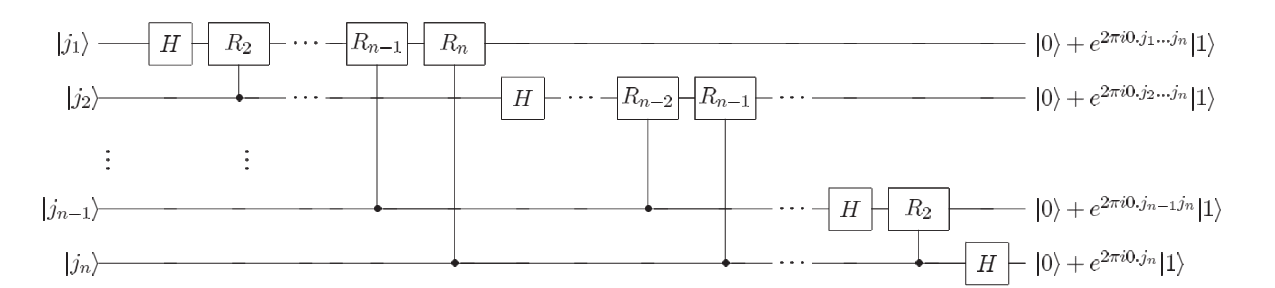
\includegraphics[width=\linewidth]{graph/QFT.png}
    \caption{General QFT Circuit}
    \label{fig:QFT}
\end{figure}
\begin{itemize}
        \item After the SWAP operations, the state of the qubits is exactly the desired output from QFT.
	\item This construction also proves that QFT is unitary since each gate in the circuit is unitary.
        \item Inverse QFT: $UU^{-1} = I$, by reversing the order of gates in quantum circuit of QFT.
	\item The best classical algorithm (FFT), which computes the DFT on $2^{n}$ elements using $\mathcal{O}(n2^{n})$ gates.
	\item How many gates does this QFT circuit use ? \\ $(1H+(n-1)\ conditional\ rotation\ gates) + (1H+(n-2)) + \cdots (1H) + \frac{n}{2}\ swap\ gate\approx \mathcal{O}(n^{2})$. (each SWAP can be done by 3 CNOTs)
	\begin{center}
	\textbf{Exponential speed up !!!}
	\end{center}
	\item Can we use QFT to speed up the computation of FT?\\
		Unfortunately, the answer is not positive $\because$ there is no known efficient way to do the following 
\begin{enumerate}
	\item Amplitudes in quantum state cannot be directly accessed by quantum measurement.
	\item In general, no known way to efficiently prepare a generic initial state to be Fourier transformed $\ket{\psi}= \sum^{}_{j} x_{j}\ket{j}$
\end{enumerate}
	\item Thus finding use for QFT is more subtle than we might have hope.
	\item Quantum algorithms find a way to use QFT and extract efficiently useful information from the quantum state.
\end{itemize}
\subsection{Quantum Phase Estimation (QPE)}
QFT is the key to a general procedure known as QPE, and QPE is the key to many quantum algorithms (e.g. quantum factoring, discrete logorithm, hidden subgroup problems) \\
\\
\textit{Question: Suppose U is a unitary operator with eigenvector $\ket{u}$ and corresponding eigenvalue $e^{2\pi i \phi_{u}}$}
\[
U\ket{u}=e^{2\pi i \phi_{u}}\ket{u}
\] 
\textit{The goal of QPE is to obtain a good estimate of $\phi_{u}$}\\
\\
Assume we have available black boxes (sometimes know as Oracle) capable of 
\begin{enumerate}
	\item Preparing the state $\ket{u}$ 
	\item Performing the controlled- $U^{2^{j}}$ (denoted as $C-U^{2^{j}}$) operations for suitable non-negative integers $j$
\end{enumerate}
This seems like a bit of a cheat: after all, in practice aren't we going to need to know how to do these things. The answer to this question is yes, and in specific examples, such as factoring, we will discuss how these black box operations are to be performed.\\
For the moment, we, at least, can think of QPE as a kind of "subroutine" or "module" that when combined with other subroutines, can be used to perform interesting computation task.
\\
QPE uses two registers
\begin{itemize}
	\item The 1st register: $t$-qubits, which will be measured to obtain our estimate about $\phi$
	\item The 2nd register: to which $U$ can be applied $U\ket{u}=e^{2\pi i \phi_{u}}\ket{u}$ contains as many qubits as is necessary to store $\ket{u}$.
\end{itemize}
How can we choose $t$ depends on 
\begin{enumerate}
	\item The number of digits of accuracy we wish to have in our estimate for $\phi$ 
	\item With what probability we wish the QPE to be successful.
\end{enumerate}

\[
\Qcircuit @C=1.4em @R=0.7em{
	\lstick{\ket{0}^{\otimes t}}& \gate{H^{\otimes t}}&\ctrl{1} & \gate{QFT^{\dagger}} &\meter \\ 
	\lstick{\ket{u}} &\qw& \gate{U^{2^j}}  &\qw& \qw &\lstick{\ket{u}}  \\ 
}
\] 
\textbf{The 1st stage: }
\[
	\left(C-U^{2^{j}}\right)\left[\frac{1}{\sqrt{2}}(\ket{0}+\ket{1})\right]\ket{u} = \frac{1}{\sqrt{2}}\left(\ket{0}\ket{u}+\ket{1}U^{2^{j}}\ket{u}\right) = \frac{1}{\sqrt{2}}\left(\ket{0}+\ket{1}e^{2\pi i 2^{j}\phi}\right)\ket{u}
\] 
Thus, the output state of the 1st region after acting on $t$-qubit is
\begin{equation*}
\begin{aligned}
&\frac{1}{\sqrt{2^{t}}}(\ket{0}+e^{2\pi i 2^{t-1}\phi}\ket{1})(\ket{0}+e^{2\pi i 2^{t-2}\phi}\ket{1}) \cdots (\ket{0}+e^{2\pi i 2^{0}\phi}\ket{1}) = \frac{1}{\sqrt{2^{t}}} \sum^{2^{t}-1}_{k=0} e^{2\pi i \phi k}\ket{k}\\
	\rightarrow & \frac{1}{\sqrt{2^{t}}} (\ket{0}+e^{2\pi i 0.\phi_{t}}\ket{1})(\ket{0}+e^{2\pi i 0.\phi_{t-1}\phi_{t}}\ket{1})\cdots(\ket{0}+e^{2\pi i 0.\phi_{1}\cdots\phi_{t-1}\phi_{t}}\ket{1})
\end{aligned}
\end{equation*}
Comparing this equation with the product form for QFT. We see that the output state after the inverse QFT is the product state $\ket{\phi_{1}\phi_{2}\cdots \phi_{t}}$ \\
\\
\textbf{The 2nd stage:} Apply the inverse QFT, i.e. QFT$^\dagger$ , on the 1st register. This is obtained by reversing the circuit for the QFT \\
\textbf{The 3rd stage:} To read out the state of the 1st register by doing a measurement in the computational basis.\\
\begin{example}
    Suppose $\phi=0.\phi_{1}\phi_{2}\cdots\phi_{t}$ can be exactly expressed in $t$ qubits.
    $$ \frac{1}{\sqrt{2^{t}}} (\ket{0} + e^{2 \pi i 0.\phi_{t}}) (\ket{0} + e^{2 \pi i 0.\phi_{t-1}\phi{t}}) \cdots (\ket{0} + e^{2 \pi i 0.\phi_{1}\phi_{2}...\phi_{t}})$$
    After $QFT^{\dagger}$, the output state is the product state $\ket{\phi} = \ket{\phi_{1}, \phi_{2}, \cdots, \phi_{t}}$.
    Hence, a measurement in the computational basis therefore gives us $\phi=\phi_{1}\phi_{2}\cdots\phi_{t}$ exactly.
\end{example}
\textbf{Summary: }
$$\frac{1}{\sqrt{2^{t}}} \sum_{k=0}^{2^{t}-1} e^{2 \pi i \phi k} \ket{k} \ket{u} \xrightarrow[]{QFT^{\dagger}} \ket{\widetilde{\phi}} \ket{u}, \quad \widetilde{\phi} \text{ is a good estimate of } \phi .$$

\paragraph{Performance and requirement (not ideal case)}\\
Above analysis applies to the ideal case where $\phi$ can be written exactly with a $t$-bit binary expression. What happens when this is not the case? $\Rightarrow$ still produces a pretty good approximation to $\phi$ with high probability. \\
Let b be the integer in the range 0 to $2^{t}-1$ such that $\frac{b}{2^{t}} = 0.b_{1}b_{2}\cdots b_{t}$ is the best t-bit approximation to $\phi$ which is less than $\phi$ . Therefore, 
\[
        \phi = \frac{b}{2^t}+\delta\, , \quad 0\leq \delta\leq\frac{1}{2^t}
\]
Suppose the outcome of the final measurement is $m$. We aim to bound the probability of obtaining $|m-b|>e$, where $e$ is positive integer characterizing our desired tolerance to error\footnote{see pages 223 and 224 of the textbook. }
\[
	P(|m-b|>e) \leq \frac{1}{2(e-1)}
\] 
Suppose we wish to approximate $\phi$ to an accuracy $2^{-n}$, i.e., we choose $t=n+p$ qubits, because
\[
e = 2^{t-n} -1  = 2^{p} -1 .
\] 
Thus,
\[
	P(|m-b|>e) \leq \frac{1}{2[(2^{p}-1)-1]}
\] 
Then, the probability of obtaining an approximation correct to this accuracy is at least
\[
	1-P(|m-b|>e) = 1-\frac{1}{2[(2^{p}-1)-1]} = 1-\epsilon
\] 
To successfully obtain $\phi$ accurate to $n$ bits with probability of success at least $1-\epsilon$, we choose
\[
	\epsilon = \frac{1}{2(2^{p}-2)} \Rightarrow 2^{p} = 2+\frac{1}{2\epsilon} \Rightarrow p = \log{\left(2+\frac{1}{2\epsilon}\right)}
\] 
Thus,
\[
	t=n+\log{\left(2+\frac{1}{2\epsilon}\right)}
\] 
\paragraph{Summary}
\begin{itemize}
    \item Input:
\begin{enumerate}
	\item A black box which performs a controlled$-U^{j}$ operation for integer $j$
	\item An eigenstate $\ket{u}$ of $U$ with eigenstate $e^{2\pi i \phi_{u}}$ 
	\item 1st register of $t=n+\log{\left(2+\frac{1}{2\epsilon}\right)}$ qubits initialized to $\ket{0}$
\end{enumerate}
\item Output: An $n$-bit approximation $\tilde{\phi_{u}}$ to $\phi_{u}$ \\
\item Runtime: $\mathcal{O}(t^{2})$ operations and one call to $C-U^{j}$ black box succeed with probability at least $1 - \epsilon$. \\

\[
\Qcircuit @C=1.4em @R=0.7em{
	\lstick{\ket{0}} & {/} \qw & \gate{H^{\otimes t}} & \ctrl{1}      & \gate{QFT^{\dagger}} & \meter \\ 	
	\lstick{\ket{u}} & {/} \qw & \qw                  & \gate{U^{j}}  & \qw         & \qw    & \lstick{\ket{u}} \\ 	
}
\] 

\begin{figure}
    \centering
    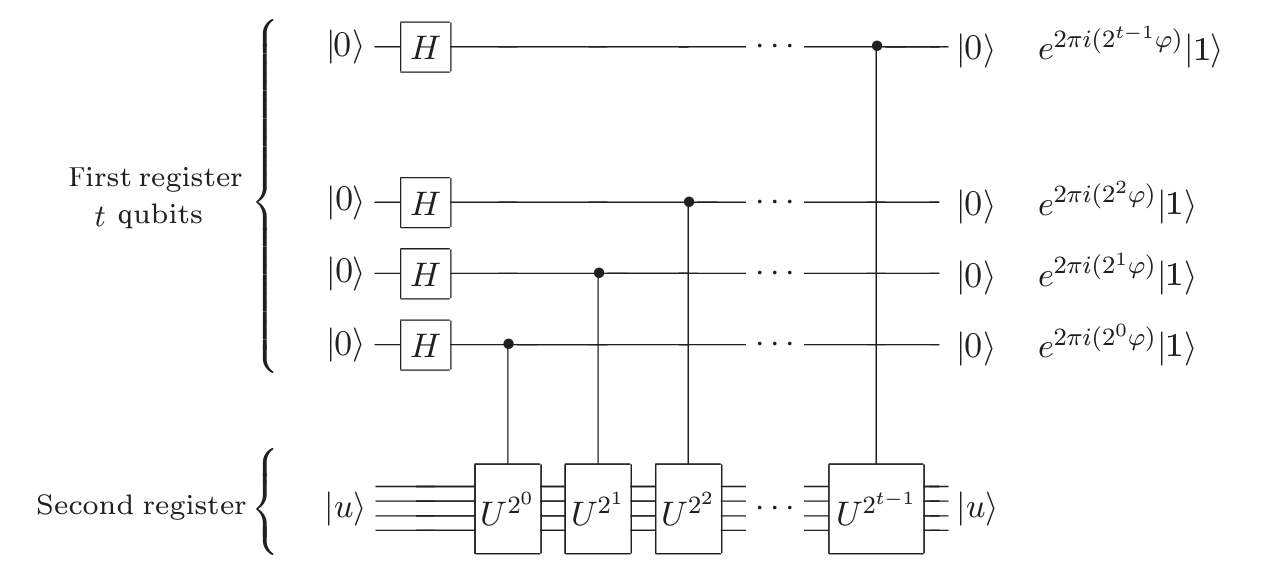
\includegraphics[width=\linewidth]{graph/QPE.png}
    \caption{General QPE Circuit for t-bits Operation}
    \label{fig:QPE}
\end{figure}

\item Procedure:
\begin{enumerate}
	\item $\ket{0}^{\otimes t}\ket{u}$ \ \ Initial state
	\item $\frac{1}{\sqrt{2^{t}}} \sum^{2^{t}-1}_{j=0} \ket{j}\ket{u}$ \ \ Create superposition
	\item $\frac{1}{\sqrt{2^{t}}} \sum^{2^{t}-1}_{j=0} e^{2\pi i j\phi_u}\ket{j}\ket{u}$ \ \ Apply black box
	\item $\ket{\tilde{\phi}}\ket{u}$ \ \ Apply inverse QFT
	\item $\tilde{\phi_{u}}$ \ \ Measure the 1st register
\end{enumerate}
\end{itemize}
\paragraph{What if we do not know how to prepare the eigenstate $\ket{u}$ of $U$?}
Suppose we prepare a state $\ket{\psi}= \sum^{}_{u} c_{u}\ket{u}, U\ket{u}=e^{2\pi i \phi_{u}}\ket{u}\therefore$ Performing the QPE procedure will give an output state close to $ \sum^{}_{u} c_{u}\ket{\tilde{\phi_{u}}}\ket{u}$, where $\tilde{\phi_{n}}$ is a pretty good approximation of $\phi_{u}$. Reading out the $1^{st}$ register will give us $\tilde{\phi}$, where  $u$ is chosen at random with probability $|c_{u}|^{2}$. This procedure allows us to avoid preparing a (possibly unknown) eigenstate out the cost of introducing some additional randomness into the algorithm.

\subsubsection{RSA Cryptosystem Protocol (Asymmetric, Public Cryptography)}
\paragraph{Fermat little Theorem:}
For a prime number $p$ and a integer $a$
$$a^{p}-a = 0 \text{ (mod }p).$$
Then if $\gcd(a, p) = 1$, 
$$a(a^{p-1}-1) = 0 \text{ (mod }p) \Rightarrow a^{p-1}-1 = 0 \text{ (mod }p).$$
\paragraph{Euler Theorem:}
$$a^{\phi(p)} = 1 \text{ (mod } p) \text{ if } \gcd(a, p) = 1$$
Note that for a prime number $p$, $\phi(p) = p-1$, and $a^{\phi(p)} = a^{p-1} = 1 \text{ (mod }p)$ reduces to Fermat little Theorem.\\
\paragraph{Mod Properties:}
\begin{itemize}
    \item $(a \pm b) \mod{N} = (a \mod{N} \pm b \mod{N}) \mod{N}$
    \item $(a \cdot b) \mod{N} = (a \mod{N})(b \mod{N}) \mod{N}$
    \item $a \cdot (b + c) \mod{N} = (ab \mod{N} +ac \mod{N}) \mod{N}$
\end{itemize}
\begin{example}
    $3^{8} \mod{7} = ((3^{2} \mod{7})^{2} \mod{7})^2 \mod{7} = (4 \mod{7})^{2} \mod{7} = 16 \mod{7} = 2$
\end{example}
\\
\paragraph{Public-key cryptosystem:} Alice wishes to create a \emph{public key} to enable people to send her messages and a \emph{matching private key} with which she can read these messages. 
\begin{enumerate}
	\item She chooses two very large enough prime number $p$ and $q$ and compute the product $N = pq$.
	\item She also picks at random a number $e<\phi(N)=(p-1)(q-1)$, which is co-prime to  $\phi(N)$, i.e. gcd$(e,\phi(N))=1$ \footnote{This is the precondition such that the modular inverse $d$ of $e$ exists, i.e. $\gcd(e, \phi(N)) = 1 \Rightarrow \exists d \text{ s.t. } ed \ \text{mod} \ \phi(N) = 1$}. $\phi(N)$ is Euler's phi function which is \# of positive integers less than $N$ which are co-prime, to $N$ . Euler's theorem $a^{\phi(N)} = 1 \ (\text{mod }N)$ if gcd$(a,N)=1$ (proof on p.631)
	\item She computes $d$ such that $ed=1 \ (\text{mod } \phi(n))$, where $d$ is called the modular multiplicative inverse.
	\item She publishes the pair $(N,e)$ as her public key, so anybody has access to it and use it to send her message.
	\item The pair $(N,d)$ is kept to herself as her private key, so only Alice can decrypt the messages that were encrypted by means of the public key.
	\item Suppose Bob wants to send a string of bits to Alice
\begin{enumerate}
	\item Breaks the message up into blocks of length $\log{N}$ bits each.
	\item Regards each single block of bits as encoding a number $x_{i},\ 0<x_{i}<N\Rightarrow$ Use the public key $(N,e)$ to encode  $x_{i}$ by $x_{i}^{e}\mod{N} = c$
\end{enumerate}
	\item To decode the encrypted block, Alice raise the message to the $d$-th power, and find a number $m < N$ s.t. $(c^{d} - m) \text{ mod } N = 0$. The $m$ obtained by it is accually $x_{i}$,\footnote{because
\[
(x_{i}^{e} \text{ mod }N)^{d} \text{ mod }N = m \text{ mod }N = (x^{e} - kN)^{d}\text{ mod }N = x_{i}^{ed} + N \cdot (\text{some integer})= x_{i}^{ed} \text{ mod }N 
\]
\[
= x_{i}^{l\cdot\phi(N)+1} \text{ mod }N  = (x_{i} \text{ mod }N) \cdot (x_{i}^{l\cdot\phi(N)} \text{ mod }N) \text{ mod }N = x_{i} \text{ mod }N\text{ (by Euler Theorem}).
\]}
\end{enumerate}
If $x_{i} \neq 0 \text{ (mod } p)$,
$$x_{i}^{ed} \text{ mod } p = x_{i}^{1+k\phi(N)} \text{ mod } p = x_{i} \cdot x_{i}^{k(p-1)(q-1)} \text{ mod } p = x_{i}(x_{i}^{p-1})^{q-1}\text{ mod } p = x_{i} \text{ mod } p$$
If $x_{i} = 0 \text{ (mod } p)$, then $x_{i}^{ed} \text{ mod } p = x_{i} \text{ mod } p$ still holds.
Similarly, $x_{i}^{ed} \text{ mod } q = x_{i} \text{ mod } q$.
So $p$ and $q$ are distinct primes, and $x_{i}^{ed} \text{ mod } N = x_{i} \text{ mod } N$.
Hence, We can ues the secret key $(N, d)$ to recover the message Bob sent to her.

\paragraph{How Secure is RSA Protocal?}
Suppose Eve is able to factor out $N=pq$ , she can then determine $\phi(N) = (p-1)(q-1)$ and find the inverse $d$ of $e$ modules  $\phi(N)$ and thus compromise the secret key.

\begin{example}
\noindent
    \begin{enumerate}
        \item Suppose Alice chooses $p=773$ and $q=739$ and $N=p\times q=571247$
        \item She picks $e=179$ , gcd$(179, \phi(N))=1$, where $\phi(N) = 569736$
        \item She computes $ed=179d=1$ (mod $\phi(N)$) and obtains $d=515627$
        \item She publishes her public key $(N,e)=(571247, 179)$
        \item She kepts $(N,d) = (517247, 515627)$ as her private key
        \item Bob write a string of bits as sequence of 6 digit numbers, \\
        $x_{i} \Rightarrow 180700 \ 100413 \ 261314 \ 192618 \ 190817 \ 170403$ encipher each block $C_{i} = x_{i}^{e} \text{ mod } N$. \\
        e.g. $x_{i} = 180700$, $C_{1} = x_{1}^{e} \text{ mod } N = 180700^{179} \text{ mod } 571247 = 141072$, and the whole message is enciphered as $141072 \ 253510 \ 459477 \ 266170 \ 286377 \ 087175$.
        \item Alice decrypt each block using her private key $d=515627$ , $c_1^d = 141072^{515627} \text{ mod }571247=180700=x_1$
    \end{enumerate}
\end{example}

\begin{remark}
    In Dec 2009, RSA-768 (768 bits, 232 digits) was factorized. Right now 1024 bits (309 digits) $\Rightarrow$ increase the security $\Rightarrow$ 2048 bits. With classical computer,  
\end{remark}
\begin{table}[h]
    \centering
    \begin{tabular}{l|c|c|c}
         \# bits & 1024 & 2048 & 4096 \\ \hline
         factoring in 2006 & $10^{5}$ years & $5 \times 10^{15}$ years& $3 \times 10^{29}$ years \\
         factoring in 2024 & 38 years & $10^{12}$ years& $7 \times 10^{25}$ years \\
         factoring in 2042 & 3 days & $3 \times 10^{8}$ years& $2 \times 10^{22}$ years \\\hline
    
        \# qubits & 5124 & 10244 & 20486 \\ \hline
        \# gates & $3\times 10^9$ & $2 \times 10^{11}$ & $\sim \times 10^{12}$ \\ 
        factoring time & 4.5 min & 36 min & 4.8 hours \\
    \end{tabular}
    % \caption{Caption}
    % \label{tab:my_label}
\end{table}

\subsection{Equivalence of factoring and order finding}
Best current method to factor a large semi-prime number on a classical computer requires  
\[
	\mathcal{O}\left(\exp{(n^{\frac{1}{3}}\log^{\frac{2}{3}}{n})}\right) \text{ operators, where $n$ is the length of $N$.}
\] 
Shor's algorithm
\[
	\mathcal{O}(n^{2}\log{n}\log{(\log{n})}) \text{ elementary gates.}
\] 

Shor's algorithm hinges on a result from number theory. The function $F(a)=x^{a} \mod{N}$ is a periodic function, where $x$ is an integer co-prime to $N$.\\
Suppose $r$ is the period of $F(a)$, we know $x^{0}\mod{N}=1$, $x^{r} \mod{N} = 1$ and $x^{2r}\mod{N}=1$
\[
	(x^{r}-1)\mod{N} = 0 \Rightarrow (x^{r/2}+1)(x^{r/2}-1) = kN = km_{1}m_{2}\Rightarrow 
\begin{aligned}
\begin{dcases}
	\text{gcd}(x^{r/2}-1,N) &= m_{1} \\
	\text{gcd}(x^{r/2}+1,N) &= m_{2} \\
\end{dcases}
\end{aligned}
\] 
Thus, it is equivalent to factoring N.

\paragraph{Order finding} For positive integers $x$ and $N$, $x<N$, with no common factors, then order $x\mod{N}$ is defined to be the least positive integer $r$ such that  $x^{r}=1 \text{ (mod } N)$.
\begin{itemize}
	\item The order finding problem is to determine the order for some specified $x$ and $N$.
	\item The order finding problem is believed to be a hard problem in a classical computer.
	\item Calculating $x^{a}$ for an exponential $\#$ of $a$'s would take exponential time on a classical computer.
	\item Shor's algorithm utilize quantum parallelism to perform the exponential number of operations in one step!! 
\end{itemize}
\paragraph{Solving order-finding using QPE} \ \\
\[
	x^{r}=1 \text{ (mod } N)
\] 
Consider the operator 
\[
	U\ket{y}=\ket{xy \text{ mod }N}\quad \forall y\in\{0,1\}^{L}, L \approx \lceil\log_{2}{N}\rceil\textit{ number of bits needed to specify N} \\
\] 
As $x$ and $N$ are co-prime, this operator $U$ is unitary\footnote{See exercise 5.12}.
\[
	x\cdot x^{r-1} = 1 \text{ (mod }N) \Rightarrow x^{r-1}\textit{ is an inverse for $x\mod{N}$}
\] 
\[
	U^{r}\ket{y}=U^{r-1}\ket{xy\mod{N}} = \ket{x^{r}y\mod{N}} = \ket{y\mod{N}} = \ket{y}.
\footnote{Computational details: If $xy \text{ mod }N = k$, then $xy = mN + k$, for arbitrary $m \in \mathbb{Z}$. For $ U^{2}\ket{y} = U\ket{xy \text{ mod }N} = \ket{x(xy \text{ mod }N) \text{ mod }N}$, $x(xy \text{ mod }N) \text{ mod }N = x (xy - mN) \text{ mod }N = x^{2}y - mNx \text{ mod }N = x^{2}y \text{ mod }N$. By mathematical induction, $U^{r}\ket{y} = \ket{x^{r}y \text{ mod }N}$}
\]
\\
Thus, $U^{r}=I$. U's eigenvalues have the form $e^{2\pi is/r}$ for some integer $s$ $\therefore$ If we can apply QPE to find  $\frac{s}{r}$, we will have obtained a considerable amount of information to help us determine $r$.\\
\\
\textit{What are the eigenvalues and eigenvectors of U?}\\
One set is 
\[
	\ket{u_s} = \frac{1}{\sqrt{r}} \sum^{r-1}_{k=0} e^{-2\pi i s k /r}\ket{x^{k}\mod{N}}\quad \forall\ 0\leq s \leq r-1 
\]
\begin{equation*}
\begin{aligned}
U\ket{u_{s}} &= \frac{1}{\sqrt{r}} \sum^{r-1}_{k=0} e^{-2\pi i s k /r}\ket{x^{k+1}\mod{N}} \\
&= \frac{1}{\sqrt{r}}  \sum^{r}_{k'=1} e^{-2\pi i s (k'-1) /r}\ket{x^{k'}\mod{N}} \\
&= e^{2\pi i s/r} \frac{1}{\sqrt{r}}  \sum^{r}_{k'=1} e^{-2\pi i s k'/r}\ket{x^{k'}\mod{N}} \\
&= e^{2\pi i s  /r}\ket{u_{s}}
\end{aligned}
\end{equation*}
Computational details: Note that $\ket{x^{r} \text{ mod }N} = \ket{x^{0} \text{ mod }N} = 1$, and $e^{2 \pi i s r/r} = e^{0} = 1$. \\$\therefore e^{2\pi i s/r} \frac{1}{\sqrt{r}}  \sum^{r}_{k'=1} e^{-2\pi i s k'/r}\ket{x^{k'}\mod{N}} = e^{2\pi i s  /r}\ket{u_{s}}$.\\
Two important requirements to be able to use QPE procedure
\begin{enumerate}
	\item Must have efficient procedure to implement a $C-U^{2}$ operation.\\
		Using a procedure known as modular exponentiation with which we can implement the entire sequence of $C-U^{2}$ operations applied by the QPE procedure using $\mathcal{O}(L^{3})$ gates.
  	\item Must be able to efficiently prepare an eigenstate $\ket{u_{s}}$ with a non-trivial eigenvalue or at least a superposition of such eigenstates.\\
	Preparing $\ket{u_{s}}$ directly requires that we know $r$, so it is impossible. Fortunately, there is a clever observation which allows us to circumvent this problem. The observation is 
\[
	\frac{1}{\sqrt{r}} \sum^{r-1}_{s=0} \ket{u_{s}} = \ket{1} \ \left(\because \sum^{r-1}_{s=0} e^{-2\pi i s k /r} = r\delta_{k0}\right)\footnote{See Exercise 5.13}
\] 
\end{enumerate}
\paragraph{Modular Exponentiation}\\
In order finding algorithm, we wish to compute 
\begin{equation*}
\begin{aligned}
	\ket{z}\ket{y}\rightarrow \ket{z}U^{z_{t}2^{t-1}}\cdots U^{z_{2}2^{1}}U^{z_{1}2^{0}}\ket{y} &= \ket{z}\ket{x^{z_{t}2^{t-1}}\cdots x^{z_{2}2^{1}}x^{z_{1}2^{0}}y\mod{N}} \\
 &= \ket{z}\ket{x^{z}y\mod{N}} = \ket{z}\ket{(x^{z}\mod{N})\quad (y\mod{N})}
\end{aligned}
\end{equation*}
Classical computation: 
\begin{enumerate}
	\item By square and multiply, a total of $(t-1)$ squaring operations at a cost of  $\mathcal{O}(L^{2})$ each. The total cost of $\mathcal{O}(L^{3})$ for the 1st stage.
	\item $x^{z}\mod{N}=(x^{z_{t}2^{t-1}}\mod{N})(x^{z_{t-1}2^{t-2}}\mod{N})\cdots (x^{z_{1}2^{0}}\mod{N})$ performing $t-1$ modular multiplications with a cost of $\mathcal{O}(L^{2})$ for each multiplication. The total cost of $\mathcal{O}(L^{3})$ for the 2nd stage\footnote{See exercise 5.14}.
\end{enumerate}
\[
\Qcircuit @C=1.4em @R=0.7em{
	\lstick{\ket{y}} & {/} \qw & \multigate{1}{U_{f}} & \rstick{\ket{y}} \qw  \\
	\lstick{\ket{z}} & {/} \qw & \ghost{U_{f}} & \rstick{\ket{z\oplus f(y)}} \qw \\
}
\] 
\begin{equation*}
\begin{aligned}
	\ket{y,0} \rightarrow \ket{y,0\oplus x^{2^{j}}y\mod{N}} &\rightarrow \ket{y\oplus x^{-2^{j}}(x^{2^{j}}y\mod{N}),x^{2^{j}}y\mod{N}}\\
 &= \ket{y\oplus y\mod{N},x^{2^{j}}y\mod{N}}\\
    &= \ket{0,x^{2^{j}}y\mod{N}}
\end{aligned}
\end{equation*}
In performing the QPE procedure, if we use $t=n+\log(2+\frac{1}{2\epsilon})$ qubits in the 1st register (e.g. $n=2L+1$) and prepare the 2nd register in the state $\ket{1}$, it follows that for each $s$ chosen uniformly at random from the range $0\leq s \leq r-1$, we will obtain an estimate of the phase $\phi\approx \frac{s}{r}$  accurate to $n=2L+1$ bits, with prob at least $\frac{1}{r}(1-\epsilon)$
\paragraph{The Continued Fraction Expansion (CF)}

How to obtain the desire answer, $r$, from the result of the QPE, $\phi\approx \frac{s}{r}$? Given that we only know $\phi$ to $n=2L+1$ bits, but we also know that it is a rational number. If we could compute the nearest such fraction to $\phi$, we might obtain $r$.
\begin{theorem}
Suppose $\frac{s}{r}$ is a rational number such that
\[
|\frac{s}{r}-\phi| \leq \frac{1}{2r^{2}}
\] 
Then $\frac{s}{r}$ is a convergent of the continued fraction for $\phi$ and can be computed in $\mathcal{O}(L^{3})$ operations using the CF algorithm.
$\because \phi$ is an approximation of $\frac{s}{r}$ accurate to $2L+1$ bits.
$$\abs{\frac{s}{r}-\phi} \leq \frac{1}{2^{2L+1}} \leq \frac{1}{2r^{2}}, \ r \leq N \leq 2^{L} $$
\end{theorem}
\begin{definition}
	A finite simple CF is defined by
\[
	[a_0,a_{1},a_{2}\cdots a_{M}] = a_{0} + \frac{1}{a_{1}+\frac{1}{a_{2}+\frac{1}{\ddots+\frac{1}{a_{M}}}}}
\] 
We define the $n^{th}$ convergent $(0\leq n\leq M)$ to this CF to be  $[a_{0},a_{1}\cdots a_{n}]$
\end{definition}
\begin{theorem}
Let $a_{0},a_{1}\cdots a_{M}$ be a sequence of positive numbers, then 
\[
	[a_0,a_{1},\cdots a_{n}]=\frac{p_{n}}{q_{n}}
\] 
where $p_{n}$ and $q_{n}$ are real numbers defined inductively by
\[
p_{0} = a_{0}\quad q_{0} = 1\,;\quad p_{1}=1+a_{0}a_{1}\quad q_{1}=a_{1}\,;\quad  p_{n} = a_{n}p_{n-1}+p_{n-2}\quad q_{n} = a_{n}q_{n-1}+q_{n-2}
\] 
\end{theorem}

\begin{example}
\[
\frac{31}{13} = 2+\frac{5}{13} = 2 + \frac{1}{\frac{13}{5}} = 2 + \frac{1}{2 +\frac{3}{5}} = 2 + \frac{1}{2 +\frac{1}{1+\frac{1}{\frac{3}{2}}}} = 2 + \frac{1}{2 +\frac{1}{1+\frac{1}{\frac{1}{1+\frac{1}{2}}}}}
\]
\[
\frac{31}{13} = [2,2,1,1,2] \Rightarrow 
\begin{matrix}
    p_0 = 2\,, & p_1 = 5\,, & p_2 = 7\,, & p_3 = 12\,, & p_4 = 31\\ 
    q_0 = 1\,, & q_1 = 2\,, & q_2 = 3\,, & q_3 =\ 5\,, & q_4 = 13
\end{matrix}
\]
\end{example}
To summarize, given $\phi$ the CF algorithm efficiently produces number $s'$ and $r'$ with no common factor such that $\frac{s'}{r'}=\frac{s}{r}$. The number $r'$ is our candidate for the order. We can check to see whether it is the order by calculating $x^{r'}\mod{N}$ and seeing if the result is 1, i.e, $x^{r'} \mod{N} \stackrel{?}{=} 1$. If so, then $r'$ is the order of $x\mod{N}$, and we are done.
\paragraph{Performance of Order-Finding Algorithm}

\textit{How can order-finding algorithm fail?}
\begin{enumerate}
	\item The QPE might produce a bad estimation to $\frac{s}{r}$. This occurs with probability at most $\epsilon$, and can be made small with negligible increase in the size of $t=n+\log(2+\frac{1}{2\epsilon})$ , $\epsilon = \frac{1}{2(2^{t-n}-2)}$.
	\item $\frac{s}{r}$ might have a common factor, then the number $r'$ returned by the CF algorithm could be a factor of $r$ and not $r$ itself.
\end{enumerate}
One way around the problem is the following. The idea is to repeat the QPE-CF procedure twice obtaining $\frac{s_{1}'}{r_{1}'}$ and $\frac{s_{2}'}{r_{2}'}$, provided that $s_{1}'$ and $s_{2}'$ have no common factors, $r$ may be extracted by taking the least common multiple of $r_{1}$ and $r_{2}$. e.g. $\frac{s_1'}{r_1'}=\frac{5}{24}=\frac{15}{48}$, $\frac{s_2'}{r_2'}=\frac{3}{16}=\frac{9}{48}$, then $r$ should be the least common multiple of 24 and 16, which is 48.


\paragraph{Summary: Quantum Order-Finding Algorithm}
\begin{enumerate}
	\item A black box $U_{x,N}$ which perform the transformation $\ket{j}\ket{k}\rightarrow \ket{j}\ket{x^{j}k\mod{N}}$ for $x$ co-prime to the $L$-bit $N$. 
	\item $t = (2L+1) + \log(2+\frac{1}{2\epsilon})$ qubits initialized to $\ket{0}$
	\item $L$ qubits initailized to $\ket{1}$ 
\end{enumerate}
Output: The least integer $r>0$ such that $x^{r}=1\mod{N}$ \\
Runtime: $\mathcal{O}(L^{3})$ operations. Succeeds with prob $\mathcal{O}(1-\epsilon)\approx \mathcal{O}(1)$\\
Procedure
\begin{enumerate}
	\item $\ket{0}\ket{1}$ initial state
	\item $\rightarrow \frac{1}{\sqrt{2^{t}}} \sum^{2^{t}-1}_{j=0}\ket{j}\ket{1} = \frac{1}{\sqrt{2^{t}r}} \sum^{2^{t}-1}_{j=0}\sum^{r-1}_{s=0}\ket{j}\ket{u_s}$ create superposition on the $1^{st}$ register.
	\item $\xrightarrow{U^j} \frac{1}{\sqrt{2^{t}}} \sum^{2^{t}-1}_{j=0} \ket{j}\ket{x^{j}\mod{N}}= \frac{1}{\sqrt{2^{t}}}\frac{1}{\sqrt{r}} \sum^{r-1}_{s=0} \sum^{2^t-1}_{j=0} e^{2\pi i s j /r}\ket{j}\ket{u_{s}}$ apply $U_{x,N}$.
	\item $\rightarrow \frac{1}{\sqrt{r}} \sum^{r-1}_{s=0} \ket{\frac{\tilde{s}}{r}}\ket{u_{s}}$ apply $QFT^{\dagger}$ to the $1^{st}$ register.
	\item $\rightarrow \frac{\tilde{s}}{r}\ket{u_{s}}$ measure the $1^{st}$ register.
	\item $\rightarrow r$ apply CF algorithm 
\end{enumerate}
Let us consider
\[
\Qcircuit @C=1.4em @R=0.7em{
	\lstick{\ket{0}} & {/} \qw & \gate{H^{\otimes t}} & \ctrl{1} & \qw & \gate{QFT^{\dagger}} & \meter \\ 	
	\lstick{\ket{1}} & {/} \qw & \qw & \gate{x^{j}\mod{N}}  & \qw &  \meter \\ 	
}
\] 
and, after the step 3 above, the circuit performs a measurement in the computational basis to determine the bit values in the $2^{nd}$ register. Suppose the result is $m$ where $m=x^{a}\mod{N}$ for some least $a \ (a \leq r)$. If $r$ is the order of $x \text{ mod }N$. Thus the measurement will select values $j=a,a+r,a+2r,...,a+(A-1)r$, where $(A-1)r$ is the greatest integer less than $\frac{2^t-a}{r}$ $(\therefore j < 2^t)$.\\
Here $a$ is fixed and has been chosen probabilistically by the choice of $m$in the measurement in the $2^{nd}$ register. The post-measurement state is
$$\ket{\phi_{s}}=\frac{1}{\sqrt{A}}\sum_{k=0}^{A-1} \ket{kr+a}\ket{m}$$
Then, apply $QFT^{\dagger} $ to the $1^{st} $ register. Let $$A=\frac{2^t}{r}, \ \ket{\psi_4} = \sqrt{\frac{1}{\left( \frac{2^t}{r} \right)}} \sum_{k=0}^{\frac{2^t}{r}-1} \ket{kr+a}\ket{m} = \sum_{2^t-1}^{k'=0} f(k') \ket{k'} \ket{m} $$.
\[
\ket{\psi_5} = (QFT^{\dagger} \otimes I) \ket{\psi_4} = \sqrt{\frac{1}{2^t}} \sum_{l=0}^{\frac{2^t}{r}-1} e^{-2\pi i \frac{(kr+a)l}{2^t}} \ket{l} \ket{m} = \sum_{l}\frac{\sqrt{r}}{2^t} \left( \sum_{k=0}^{\frac{2^t}{r}-1} e^{-2\pi i \frac{krl}{2^t}} \right) e^{-2\pi i \frac{al}{2^{t}}} \ket{l} \ket{m} 
\]
\[
= 
\begin{cases}
    \sum_{l=0}^{2^t-1} \sqrt{\frac{1}{r}} e^{-2\pi i \frac{al}{2^t}} \ket{l} \ket{m}, \text{ if } l=n \frac{2^t}{r} \\
    0, \text{ otherwise}.
\end{cases}
\]

i.e., the inverse Fourier transform of a state with period $r$ is a state with period $\left( \frac{2^t}{r} \right)$
$$\psi_s = \frac{1}{\sqrt{r}} \sum e^{-2\pi i a \frac{s}{r}} \ket{s \frac{2^{t}}{r}} \ket{m} $$
Measuring register 1 and suppose use get a value $C=s\frac{2^t}{r}$ with $s=0$, $r=1$ chosen equiprobably
$$\ket{\psi_s} = \ket{s\frac{2^t}{r}}\ket{m}, \ \frac{C}{2^t} = \frac{s}{r}.$$
Lastly, apply the CF algorithm to find $r$.

\paragraph{Summary: Reduction of factoring to order finding}\\
Inputs: A composite integer number $N$.\\
Outputs: A non-trivial factors of $N$.\\
Runtime: $\mathcal{O}(L^3)$ operations succeeds with prob. $\mathcal{O}(1)$.\\
Procedure:
\begin{enumerate}
    \item Determine if $N$ is a prime, an even integer or an integer power of a prime number.( $N=a^b$ for integers $a \geq 1$ and $b \geq 2$, if so, return the factor $a$.) This step would be performed on a classical computer.
    \item Randomly choose $x$ that is co-prime to $N$ for $1 \leq x \leq N-1$. If $\gcd(x,N)>1$ then return the factor. This step would be done on a classical computer.
    \item Use the order-finding subroutine to find the order $r$ of $x$ module $N$. This step will be done on a quantum computer.
    \item If $r$ is even and $x^{r/2} \neq -1 \text{ (mod }N)$, then  compute $\gcd(x^{r/2}-1, N)$ and $\gcd(x^{r/2}+1,N)$ and test to see if one of these is a non-trivial factor. If so, return the factor. Otherwise, the algorithm fails, and go back to step 2. This final step  can be done on a classical computer.
\end{enumerate}

\paragraph{Example 1}
    Factoring $N=15$ quantum-mechanically: (use of ordering finding QPE and CF algorithm)
    \begin{enumerate}
        \item $N$ is not even, continue. $N \neq a^b$ so continue.
        \item Choose a random numbers which is co-prime to $N$. Suppose we choose $x=7$, $\gcd(x,N)=\gcd(7,15)=1$ so continue.
        \item Choose $t=11$ qubits for register 1 and $L=4$ qubits for register 2. $t=n+\log(2+\frac{2}{2\epsilon}), \ n=2L+1=9$. Choosing $t=11$ ensures an error probability $\epsilon$ of at most $\frac{1}{4}$ .
        $$\ket{\psi_1} = \ket{0000000000 \ 0001}$$
        \item $\ket{\psi_s} $ create superposition on register 1, so we get $\psi_s = \frac{1}{\sqrt{2^t}} \sum_{j=0}^{2^t-1} \ket{j}\ket{1} = \frac{1}{\sqrt{2048}}(\ket{0}+\ket{1}+\ket{2}+...+\ket{2047})\ket{1} $.
        \item Apply $C-U^{j}_{x,N} $ on $\ket{\psi_s}$ to compute $x^j \text{ mod }N=15$, leaving the result in the $2^{nd}$ register.
        $$\ket{\psi_s} = \frac{1}{\sqrt{2048}} (\ket{0}\ket{1}+\ket{1}\ket{7}+\ket{2}\ket{4}+\ket{3}\ket{13}+\ket{4}\ket{1}+\ket{5}\ket{7}+\ket{6}\ket{4}+\ket{7}\ket{13}+\ket{8}\ket{1}+\ket{9}\ket{7}+...).$$ (The period $r$ of $7^x \text{ mod }15$ is 4.)
        \item Measuring the $2^{nd}$ register and randomly get 4, leaving the post-measurement state to be
        $$\ket{\psi_s} = \frac{1}{\sqrt{||A||}} (\ket{2}+\ket{6}+\ket{10}+\ket{14}+...+\ket{2044})\ket{4}, \ ||A||=512$$
        \item Apply $QFT^{\dagger}$ on the $1^{st}$ register,
        $$\ket{\psi_s}=\frac{1}{\sqrt{4}}(\ket{0}-\ket{512}+\ket{1024}-\ket{1536})\ket{4}$$
        \item Measuring the $1^{st}$ register. All the possible state has the same probability to be measured, which is $\frac{1}{4}$.
        Suppose we obtain $C=1536$,
        \[
        \frac{C}{2^t}=\frac{1536}{2048}=\frac{1}{1+\frac{1}{3}}=[0,1,3] \Rightarrow 
        \begin{matrix}
            p_0 = 0\,, & p_1 = 1\,, & p_2 = 3 \cdot 1 + 0 = 3\\
            q_0 = 1\,, & q_1 = 1\,, & q_2 = 3 \cdot 1 + 1 = 4
        \end{matrix}
        \]
        Check: $\abs{\frac{1536}{2048}-\frac{p_n}{q_n}} \leq \frac{1}{2^{2L+1}} = \frac{1}{2^9}$.
        $\therefore \frac{p_n}{q_n}=\frac{3}{4}=\frac{s'}{r'} \Rightarrow r'=4$ as the order of $x=7 \text{ mod }15$.
        \item By chance $r$ is even and more over $ x^{r/2} \text{ mod }N=7^2 \text{ mod }15 = 4 \neq -1$ . So the algorithm works. Then compute $\gcd(7^2-1,15)=3, \ \gcd(7^2+1,15)=5$. Now by testing $3 \times 5 = 15 = N$, we see we have now found the factors of 15.
    \end{enumerate}
    For $N=15$, and $\gcd(x,15)=1$, $x$ could be any numbers from the set \{2, 4, 7, 8, 11, 13, 14\}. Let us pick $x=11$, and compute $x^j \text{ mod }15$,
    $$\ket{\psi_s} = \frac{1}{\sqrt{2048}}(\ket{0}\ket{1}+\ket{1}\ket{11}+\ket{2}\ket{1}+\ket{3}\ket{11}+\ket{4}\ket{1}), \ \therefore r=2.$$
    $$\gcd(11^{2/2}-1,15)=5, \ \gcd(11^{2/2}+1,15)=3.$$
    So $3 \times 5 = 15$, verified again.
    Respectively, orders modulo 15 or element \{2, 4, 7, 8, 11, 13, 14\} are \{4, 2, 4, 4, 2, 4, 2\}, except $x=14$, we obtains $r=2$, $x^{r/2}=14^{2/2}=14=-1 \ (\text{mod} \ 15), \ \gcd(x^{r/2}+1,N)=N$.

\paragraph{Example 2}
    Factoring \textbf{$N=55$} quantum-mechanically: (use of ordering finding QPE and CF algorithm)
    \begin{enumerate}
        \item $N$ is not even, continue. $N \neq a^b$ so continue.
        \item Choose a random numbers which is co-prime to $N$. Suppose we choose \textbf{$x=13$}, \textbf{$\gcd(x,N)=\gcd(13,55)=1$} so continue.
        \item Choose \textbf{$t=13$} qubits for register 1 and \textbf{$L=6$} qubits for register 2. 
        $$\ket{\psi_1} = \ket{000000000000\ 000001}$$
        \item $\ket{\psi_s} $ create superposition on register 1, so we get $\psi_s = \frac{1}{\sqrt{2^t}} \sum_{j=0}^{2^t-1} \ket{j}\ket{1} = \frac{1}{\sqrt{8192}}(\ket{0}+\ket{1}+\ket{2}+...+\ket{8191})\ket{1} $.
        \item Apply $C-U^{j}_{x,N} $ on $\ket{\psi_s}$ to compute $x^j \text{ mod }N=55$, leaving the result in the $2^{nd}$ register.
        $$\ket{\psi_s} = \frac{1}{\sqrt{2048}} (\ket{0}\ket{1}+\ket{1}\ket{13}+\ket{2}\ket{4}+...+\ket{9}\ket{28}+...+\ket{20}\ket{1}+...+\ket{8192}\ket{2}).$$ (The period $r$ of $13^x \text{ mod }55$ is \textbf{20}.)
        \item Measuring the $2^{nd}$ register and randomly get \textbf{28}, leaving the post-measurement state to be
        $$\ket{\psi_s} = \frac{1}{\sqrt{||A||}} (\ket{9}+\ket{29}+\ket{49}+...+\ket{8189})\ket{28}, \ ||A||=410$$
        \item Apply $QFT^{\dagger}$ on the $1^{st}$ register, The frequency domain would be an envelope instead of a few nice peaks. 
        \item \emph{(Something Wrong from here)} Measuring the $1^{st}$ register. 
        Suppose we obtain $C=4915$ (prob $\approx$ 4.4\%),
        \[
        \frac{C}{2^t}=\frac{4915}{8192}=\frac{1}{1+\frac{1}{\frac{1}{1+\frac{1}{2+\frac{1}{1637}}}}}=[0,1,1,2,1637] \Rightarrow 
        \begin{matrix}
            p_0 = 0\,, & p_1 = 1\,, & p_2 = 4912\\
            q_0 = 1\,, & q_1 = 1\,, & q_2 = 8187
        \end{matrix}
        \]
        Check: $\abs{\frac{4915}{8192}-\frac{p_n}{q_n}} \leq \frac{1}{2^{2L+1}} = \frac{1}{2^{13}}$.
        $\therefore \frac{p_2}{q_2}=\frac{3}{5}=\frac{s'}{r'} \Rightarrow r'=5$ as the order of $x=13 \text{ mod }55$
        \item By chance $r$ is odd, so repeat the algorithm and suppose we got the same result until step 7. In step 8, we get $C=409$ 
        \[
        \frac{C}{2^t}=\frac{409}{8192}=\frac{1}{20+\frac{1}{\frac{1}{34+\frac{1}{12}}}}=[0,20,34,12] \Rightarrow 
        \begin{matrix}
            p_0 = 0\,, & p_1 = 1\,, & p_2 = 34\\
            q_0 = 1\,, & q_1 = 20\,, & q_2 = 681
        \end{matrix}
        \]
        Check: $\abs{\frac{409}{8192}-\frac{p_n}{q_n}} \leq \frac{1}{2^{2L+1}} = \frac{1}{2^{13}}$.
        $\therefore \frac{p_1}{q_1}=\frac{1}{20}=\frac{s'}{r'} \Rightarrow r'=20$ as the order of $x=13 \text{ mod }55$.
        By chance $r$ is even, and more over $x^{r/2} \text{ mod }N = 13^{10} \text{ mod }55 \neq -1$. So the algorithm works. Then compute $\gcd(13^{10}-1,55)=5, \ \gcd(13^{10}+1,15)=11$. Now by testing $5 \times 11 = 55 = N$, we see we have now found the factors of 55.
    \end{enumerate}
    
\section{Quantum Search Algorithm}
Grover's Algorithm (1997)\footnote{Grover Algorithm with zero theoretical failure rate
, G.L Long, Phys. Rev. A64 (2001) 022307}\footnote{F.M. Toyama et al. Information Processary, 12, 1897 (2013).}: Good for unsorted database. e.g. search for the name in telephone book (which is sorted by name) by phone number.
$$\text{Name} \xrightarrow{easy} \text{Phone Number}$$
$$\text{Phone Number} \xrightarrow{hard} \text{Name}$$
If there are $N$ entries in the phone book, it will take an average of $\frac{N}{2}$ queries ($\mathcal{O}(N)$) to find the name. The search time is linear with respect to the size "$N$" of the phonebook. That is because the number of possible inputs scales linearly with the size of the problem.

\begin{example}
    Factoring a large semi-prime number $N=pq$.\\
    One possible way: Search all number from 2 through $N^{\frac{1}{2}}$ for the smaller of the two prime factors. That is, we successively do a trial divisor of $N$ by each number in the range 2 to $N^{\frac{1}{2}}$, until we find the smaller prime factor.
    \begin{itemize}
        \item This search-based method require $\mathcal{O}(N^{\frac{1}{2}})$ trail divisors to find a factor.
        \item The quantum search algorithm can be used to speed up this process, $\mathcal{O}((N^{\frac{1}{2}})^{\frac{1}{2}})=\mathcal{O}(N^{\frac{1}{4}})$.
    \end{itemize}
\end{example}

\subsection{What is Grover's Algorithm?}
Suppose we wish to search through a search space of $N$ elements $N=2^n$, and that the search problem has exactly $M$ solutions, with $1 \leq M \leq N$.\\
Quantum Oracle:
\begin{equation*}
\begin{aligned}    
    f:&x            &\, \rightarrow &f(x)\\
      &\{0,1\}^n      &            & \{0,1\}\\
      &0\leq x\leq N-1&            &\\
\end{aligned}
\end{equation*}

\[
\text{By definition, } 
\begin{cases}
    f(x)=1\text{, if $x$ is a solution.}\\
    f(x)=0\text{, if $x$ is not a solution.}
\end{cases}
\]

The problem is to find solutions with minimum number of queries of the Oracle of $\mathcal{O}$ : defined by its action on the computational basis \\
\begin{minipage}{0.3\linewidth} 
\[
\Qcircuit @C=1.4em @R=0.7em{
	\lstick{\ket{x}} & \qw & \multigate{1}{U_{f}} & \rstick{\ket{x}} \qw  \\
	\lstick{\ket{q}} & \qw & \ghost{U_{f}} & \rstick{\ket{q\oplus f(x)}} \qw \\
}
\] 
\end{minipage}
\begin{minipage}{0.5\linewidth} 
\[
\Qcircuit @C=1.4em @R=0.7em{
	\lstick{\ket{x}} & \qw & \multigate{1}{U_{f}} & \rstick{\ket{x}} \qw  \\
	\lstick{\ket{0}} & \qw & \ghost{U_{f}} & \rstick{\ket{f(x)}} \qw  \\
}
\] 
\end{minipage}
check if $x$ is a solution by checking if the oracle qubit has been flipped to $\ket{1}$ \\
Just as was done in the Deutsch-Jozsa algorithm, it is useful to apply the oracle qubit initially in the state $\frac{\ket{0}-\ket{1}}{\sqrt{2}}.$\\

\[
\Qcircuit @C=1.4em @R=0.7em{
	\lstick{\ket{x}} & \qw & \multigate{1}{U_{f}} & \rstick{(-1)^{f(x)}\ket{x}} \qw  \\
	\lstick{\frac{\ket{0}-\ket{1}}{\sqrt{2}}} & \qw & \ghost{U_{f}} & \rstick{\frac{\ket{0}-\ket{1}}{\sqrt{2}}} \qw &  \\
}
\]\\

$$\ket{x}\ket{-}\xrightarrow{\mathcal{O}}\ket{x}\frac{\ket{0\oplus f(x)}-\ket{1\oplus f(x)}}{\sqrt{2}}
=\ket{x}\frac{\ket{f(x)-\ket{1\oplus f(x)}}}{\sqrt{2}}
= \ket{x}(-1)^{f(x)}\ket{-}.\footnote{The state of the Oracle qubit is not changed throughout the Q. search algorithm.}$$

We may say that the Oracle "marks" the solution to the search problem by shifting the phase of the solution.
\begin{itemize}
    \item For an $N$-item search problem with $M$ solutions, it turns out that we need only apply the search Oracle $\mathcal{O}(\sqrt{\frac{N}{M}})$ times in order to obtain a solution on a Q. computer.
    \item It seems as though the oracle already knows the answer to the search problem: What possible use could it be to have a Q search algorithm based upon search Oracle consultation?
    \item The answer is that there is a distinction between "knowing"  the solution to a search  problem and being able to "recognize" the solution  to the search problem. 
    \item It is possible to be able to recognize the solution without being able to know the solution. 
\end{itemize}
e.g. Factoring
\begin{itemize}
    \item The action of the Oracle upon input of the state $\ket{x}$ is to divide $N$ by $x$ , and check to see of the division is exact. Flip the oracle qubit if this is so.
    \item Even without knowing the prime factor of $N$, we can explicitly construct an Oracle which recognize a solution to the search problem when it sees one.
    \item The factoring example is computationally interesting but not practical. There are classical algorithm for factoring which work much faster than searching all possible divisions.
\end{itemize}
\subsection{The Procedure of Quantum Search Problem}
\[
\Qcircuit @C=1.4em @R=0.7em{
	\lstick{\ket{0}} & {/} \qw & \gate{H^{\otimes}} & \multigate{1}{G} & \qw & \multigate{1}{G} & \qw & \meter \\
	\lstick{\text{Oracle workspace}} & {/} \qw & \qw & \ghost{G} & \qw & \ghost{G} & \qw & \text{...} \\
}
\]

\begin{minipage}{0.3\linewidth}
\[
\Qcircuit @C=1.4em @R=0.7em{
        \qw & \multigate{4}{G} & \qw \\
        \qw & \ghost{G} & \qw \\
        \qw & \ghost{G} & \qw \\
        \qw & \ghost{G} & \qw \\
        \qw & \ghost{G} & \qw
}
\]
\end{minipage}
=
\begin{minipage}{0.3\linewidth}
    \[
\Qcircuit @C=1.4em @R=0.7em{
        \qw & \multigate{4}{\mathcal{O}\ket{x}\rightarrow (-1)^{f(x)}\ket{x}} & \multigate{2}{H^{\otimes n}} & \multigate{2}{\ket{x}\rightarrow -\ket{x} for x > 0} & \multigate{2}{H^{\otimes n}}\\
        \qw & \ghost{\mathcal{O}\ket{x}\rightarrow (-1)^{f(x)}\ket{x}} & \ghost{H^{\otimes n}} & \ghost{\ket{x}\rightarrow -\ket{x} for x > 0} & \ghost{H^{\otimes n}}\\
        \qw & \ghost{\mathcal{O}\ket{x}\rightarrow (-1)^{f(x)}\ket{x}} & \ghost{H^{\otimes n}} & \ghost{\ket{x}\rightarrow -\ket{x} for x > 0} & \ghost{H^{\otimes n}}\\
        \qw & \ghost{\mathcal{O}\ket{x}\rightarrow (-1)^{f(x)}\ket{x}} &\qw &\qw &\qw \\
        \qw & \ghost{\mathcal{O}\ket{x}\rightarrow (-1)^{f(x)}\ket{x}} &\qw &\qw &\qw
}
\]

\end{minipage}

\begin{itemize}
    \item The Oracle may employ work qubits for its implementation, but the analysis of the Q. search algorithm involves the $n$-qubits register.
    \item The Q. algorithm consists of repeated application of a Q. solution, known as Grover iteration or Grover operator, $G$.
\end{itemize}

Grovers iteration operator:
\begin{enumerate}
    \item Apply the Oracle $\mathcal{O}$.
    \item Apply the Hadamard transform $H^{\otimes n}$.
    \item Perform a conditional phase shift, with every computational basis state except $\ket{0}$ receiving a phase of ($-1$): $\ket{x}\rightarrow -(-1)^{\delta_{0x}}\ket{x}$.
    \item Apply the Hadamard transform $H^{\otimes n}$.
\end{enumerate}
%put the n-qubit toffli gate diagram here.
One way to implement $\ket{x}\rightarrow (-1)^{\delta_{x0}}\ket{x}$ is:
$$-(-1)^{\delta_{x0}}\ket{x} = (2\ket{0}\bra{0}-I)\ket{x}$$
Note that $H^{\otimes n}\ket{0}=\frac{1}{\sqrt{2^n}}\sum_{x=0}^{2^n-1} \ket{x} = \frac{1}{N}\sum_{x=0}^{N-1}\ket{x}=\ket{\psi} $.
The combined effect of (2), (3) and (4) is:
$$H^{\otimes n}(2\ket{0}\bra{0}-I)H^{\otimes n} = 2\ket{\psi}\bra{\psi} - I, \ \therefore G=(2\ket{\psi}\bra{\psi}\otimes I-I\otimes I)\mathcal{O}$$

Geometric Visualization:\\
Let $\ket{\alpha}=\frac{1}{\sqrt{N-M}}\sum_{x:f(x)=0} \ket{x} $ and $\ket{\beta} = \frac{1}{\sqrt{M}}\sum_{x:f(x)=1} \ket{x} $ \footnote{A sum over all $x$ which are solution to the search problem.}

$$\ket{\psi}=\frac{1}{\sqrt{N}}\sum_{x=0}^{N-1} \ket{x} = \sqrt{\frac{N-M}{N}} \ket{\alpha} + \sqrt{\frac{M}{N}} \ket{\beta} = \cos{\frac{\theta}{2}} \ket{\alpha} + \sin{\frac{\theta}{2}}\ket{\beta}$$
where
$$\cos{\frac{\theta}{2}}=\sqrt{\frac{N-M}{N}}, \ \sin{\frac{\theta}{2}}=\sqrt{\frac{M}{N}}.$$
Oracle:
$$\mathcal{O}(a\ket{\alpha}+b\ket{\beta}) = a\ket{\alpha}-b\ket{\beta}, \ \mathcal{O} = I-2\ket{\beta}\bra{\beta}.$$
$$( I-2\ket{\beta}\bra{\beta} ) ( a\ket{\alpha}+b\ket{\beta} )
= (a\ket{\alpha}+b\ket{\beta}) - 2 b \ket{\beta} = a\ket{\alpha}-b\ket{\beta}.$$
$\mathcal{O}$ performs a reflection about the hyperplane perpendicular to $\ket{\beta}$ (i.e. about the vector $\ket{\alpha}$ in the plane defined by $\ket{\alpha}$ and $\ket{\beta}$). If we change $\ket{\beta}$ to arbitrary $\ket{\psi} = a\ket{\alpha}+b\ket{\beta}$, we can reflect 
the about the vector $\ket{\psi}$ on the hyperplane.\\
\begin{figure}
    \centering
    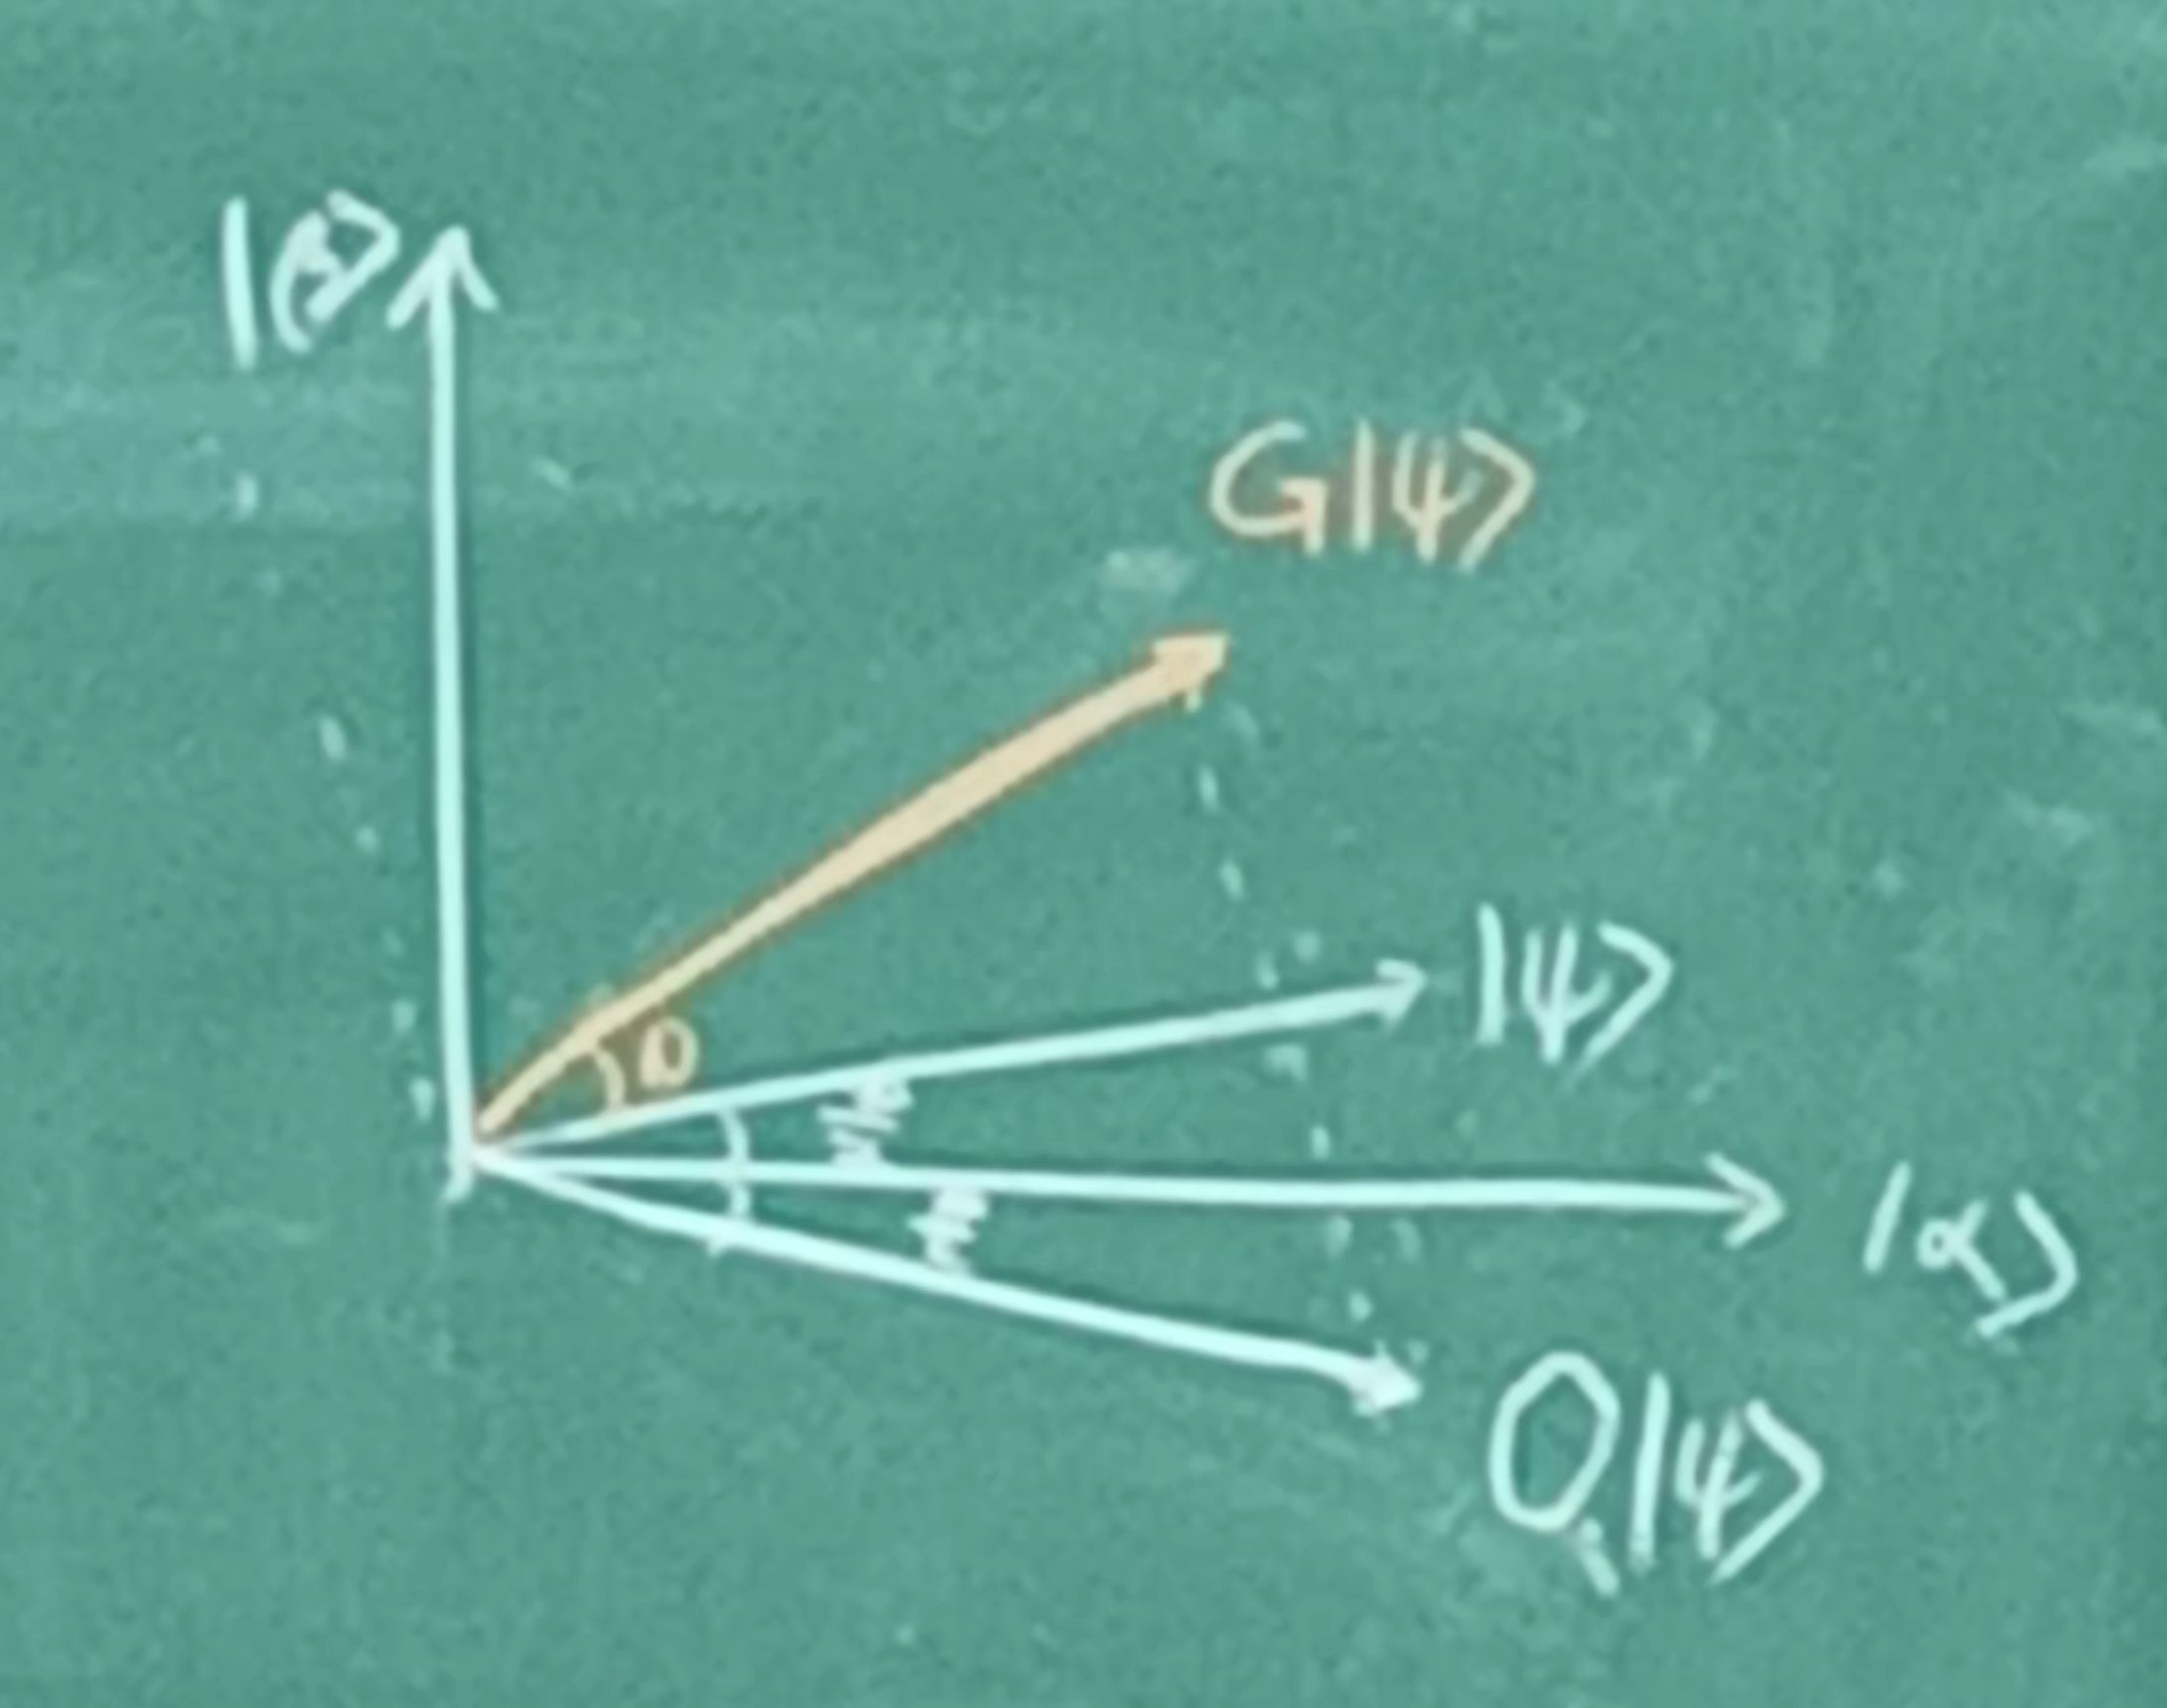
\includegraphics[width=.4\linewidth]{graph/20231207_162134.jpg}
    \caption{reflection operation}
    \label{fig:enter-label}
\end{figure}
The product of the two reflection is actually a rotation!
$$G\ket{\psi}=\cos{\frac{3\theta}{2}}\ket{\alpha} + \sin{\frac{3\theta}{2}}\ket{\beta}
= \cos{\left(\theta + \frac{\theta}{2}\right)}\ket{\alpha} + \sin{\left(\theta + \frac{\theta}{2}\right)}\ket{\beta}$$
$$\therefore G=
    \left[
\begin{matrix}
    \cos{\theta} & -\sin{\theta} \\
    \sin{\theta} & \cos{\theta} \\
\end{matrix}
    \right]
, \ \sin{\theta} = 2 \sin{\frac{\theta}{2}}\cos{\frac{\theta}{2}} = \frac{2\sqrt{M(N-M)}}{N}
$$

Continued application of $G$ takes the state $\ket{\psi}$ to $G^k\ket{\psi} = \cos((k+\frac{1}{2})\theta)\ket{\alpha} + \cos((k+\frac{1}{2})\theta)\ket{\beta}$\\

Summary:
\begin{enumerate}
    \item $G$ is a rotation in the 2-D space spanned by $\ket{\alpha}$ and $\ket{\beta}$, rotating the is the space by Q. radians per application of $G$.
    \item Repeated application of the Grover iteration $G$rotates the state vector close to $\ket{\beta}$.
    \item When this occurs, an observation in the computational basis produces with high probability that one of the outcome superposed in $\ket{\beta}$, that is, a solution to the search problem. 
\end{enumerate}

\subsection{Performance}
How many times must the $G$ be repeated in order to rotate $\ket{\psi}$ near $\ket{\beta}$ ?
\[
    R = CI\left[\frac{\frac{\pi}{2}-\frac{\theta}{2}}{\theta}\right] = CI\left[\frac{\cos^{-1}\sqrt{\frac{M}{N}}}{\theta}\right]
\]
where $CI\left[y\right]$ denotes the integer close to the real number $y$ , by convection $CI(3.5)=3$ . The worst situation: $\frac{\frac{\pi}{2}-\frac{\theta}{2}}{\theta}=\frac{1}{2} \Rightarrow \frac{\theta}{2} = \frac{\pi}{4}$

\begin{itemize}
    \item Observation of the  state in the computational basis yields a solution with probability 
    \[
        \sin^{2}\left(\left(k+\frac{1}{2}\right)\theta\right) \geq \sin^{2}\left(\frac{\pi}{4}\right) = \frac{1}{2}
    \]
    \item For $M << N$, we have $\sin{\frac{\theta}{2}=\sqrt{\frac{M}{N}}} \approx \frac{\theta}{2}, \ \therefore$ the angular-error in the final state is at most $\frac{\theta}{2} \approx \sqrt{\frac{M}{N}}$ giving a probability of error of at most $\frac{M}{N}$. Hence, $R \leq \left[\frac{\frac{\pi}{2}}{\theta}\right]=\left[\frac{\pi}{2\theta}\right]$, lower bound on $\theta$ will give an upper bound on $R$. For $M \leq \frac{N}{2}$, we have $\frac{\theta}{2} \geq \sin{\frac{\theta}{2}} = \sqrt{\frac{M}{N}}$.
    Therefore, the upper bound in the number of the Grover iteration required $R \leq \left[\frac{\pi}{2}\sqrt{\frac{N}{M}}\right]$.\\
    That is, $R\approx \mathcal{O}(\sqrt{\frac{M}{N}})$, Grover iteration (and thus Oracle calls) must be performed in order to obtain a solution to the search problem with high probability, a quadratic improvement over $\mathcal{O}(\frac{M}{N})$ oracle calls required classically.
\end{itemize}

\subsubsection{Summary: Q. Search Algorithm for the Case $M=1$}
Inputs: 
\begin{enumerate}
    \item A black box oracle $\mathcal{O}$ which perform the transformation $\mathcal{O}\ket{x}\ket{g}=\ket{x}\ket{g\oplus f(x)}$, where $f(x)=0$ for all $0 \leq x \leq 2^n$.
    \item $n+1$ qubits in state $\ket{0}$.
\end{enumerate}
Outputs: $x_0$\\
Runtime: $\mathcal{O}(\sqrt{N})=\mathcal{O}(\sqrt{2^n})$ operators. Succeed with prob. $\mathcal{O}(1)$.\\
Procedure:
\begin{enumerate}
    \item $\ket{0}^{\otimes n}\ket{0}$ initial state.
    \item $\frac{1}{\sqrt{2^n}}\sum_{x=0}^{2^n-1}\ket{x}\ket{-} $
    \item $[(2\ket{\psi}\bra{\psi}-I)\mathcal{O}]^R\frac{1}{\sqrt{2^n}} \sum_{x=0}^{2^n-1} \ket{x}\ket{-} \approx \ket{x_0}\ket{-}$ (apply the $G$ $R=\left[\frac{\pi\sqrt{2^n}}{4}\right]$ times).
    \item $x_0$ (measure the last register).
\end{enumerate}

\paragraph{Example}
Search one solution on a search space of size $N=4$ . $f(x)=0, \ \forall x \neq x_0$ , in which case $f(x_{0}) = 1$.
For $M=1$, $N=4$, $\sin{\frac{\theta}{2}}=\frac{1}{2} \Rightarrow \theta= \frac{\pi}{3}, \ \frac{\theta}{2}=\frac{\pi}{6}$, and $\frac{\pi}{3}+\frac{\pi}{6}=\frac{\pi}{2}$. So, only exactly one iteration is required!

\[
\Qcircuit @C=1.4em @R=0.7em{
	\lstick{\ket{0}} & \qw & \qw      & \gate{H} & \multigate{2}{oracle} & \gate{H} & \rstick{} \qw  \\
	\lstick{\ket{0}} & \qw & \qw      & \gate{H} & \ghost{oracle}        & \gate{H} & \rstick{} \qw &  \\
        \lstick{\ket{0}} & \qw & \gate{X} & \gate{H} & \ghost{oracle}       & 
}
\]

For $x_0=2$
\[
\Qcircuit @C=1.4em @R=0.7em{
\qw & \ctrl{1} & \qw\\
\qw & \ctrlo{1} & \qw\\
\qw & \targ & \qw\\
}
\]

For $x_0=0$
\[
\Qcircuit @C=1.4em @R=0.7em{
\qw & \ctrlo{1} & \qw\\
\qw & \ctrlo{1} & \qw\\
\qw & \targ & \qw\\
}
\]

Classically, $1\times \frac{1}{4} + 2\times\frac{3}{4}\frac{1}{3}+3\times\frac{3}{4}\frac{2}{3}\cdot 1 = 2.25$ oracle queries on average. 
What happen when $M\geq \frac{N}{2}$
\[
    \sin \frac{\theta}{2} = \sqrt{\frac{M}{N}} \, , \quad \cos \frac{\theta}{2} = \sqrt{\frac{N-M}{N}}
\]
\[
    \sin \theta = 2\sin \frac{\theta}{2} \cos \frac{\theta}{2} = 2\sqrt{\frac{M}{N}} \sqrt{\frac{N-M}{N}}
\]
\[
    \theta = \sin^{-1} \left(\frac{2\sqrt{M(N-M)}}{N}\right)
\]
Suppose $\frac{N}{2} \leq M \leq N$ , as $M$ varies from $\frac{N}{2}$ to $N$ , $\theta$ gets smaller. The number of iteration $R= CI \left[\frac{\cos^{-1}\sqrt{\frac{M}{N}}}{\theta}\right]$ increases with $M$ for $M\geq \frac{N}{2}$ .
\begin{enumerate}
    \item If $M \geq \frac{N}{2}$ is known in advance, we can just randomly pick an item and check whether it is a solution using the Oracle.
    \item If the number of solution is not known, the idea is to double the number of elements in the search space, by adding $N$ extra items to the search space, none of which are solution. This is effected by adding a single qubit $\ket{q}$ to the search index doubling the number of item to be searched to $2N$.
\end{enumerate}
\paragraph{Quantum Counting}
How quickly can we determine the number of solution $M$ to an $N$ item search problem if $M$ is not known in advance? Classically, $\mathcal{O}(N)$ consultation (queries)
Quantumly, combining the Grover iteration with QPE
\begin{enumerate}
    \item Counting the number of solutions $M$ (determine $M=0$ or not)
    \item Apply the quantum search algorithm to find a solution
\end{enumerate}


Grover: $$G=
\left[
\begin{matrix}
    \cos{\theta} &-\sin{\theta} \\
    \sin{\theta} &\cos{\theta}
\end{matrix}
\right]$$
eigenvalue:
\begin{align*}
    e^{i\theta} &,  \ \ket{\alpha} = \frac{1}{\sqrt{2}}(i\ket{\alpha}+\ket{\beta})\\
    e^{i(2\pi-\theta)} &,  \ \ket{\beta} = \frac{1}{\sqrt{2}}(-i\ket{\alpha}+\ket{\beta})
\end{align*}
expanding the size of search space to $2N$, therefore, $\sin{\frac{\theta}{2}}=\sqrt{\frac{M}{2N}}$.
\[
\Qcircuit @C=1.4em @R=0.7em{
    \qw & \qw & \multigate{2}{H^{\otimes t}} & \qw & \qw & \qw & \ctrl & \qw & \multigate{2}{QFT^{\dagger}} & \qw & \meter      \\
    \qw & \qw & \ghost{H^{\otimes t}} & \qw & \qw & \ctrl & \qw & \qw & \ghost{QFT^{\dagger}} & \qw & \meter \\
    \qw & \qw & \ghost{H^{\otimes t}} & \qw & \ctrl & \qw & \qw & \qw & \ghost{QFT^{\dagger}} & \qw & \meter \\
    \lstick{\ket{0}} & {/} \qw & \gate{H^{\otimes n+1}} \qw & \gate{G} & \gate{G} & \gate{G} & \qw &\qw&\qw&\qw&\qw \\
}
\]

$$t=m+\log(2+\frac{2}{\epsilon}) \text{ bits.}, \ \sin^2{\frac{\theta}{2}}=\frac{M}{2N}$$
QPE circuit is to estimate $\theta$ to $m$ bits of accuracy with prob. of success at least $1-\epsilon$.



\end{document}
